% !TeX spellcheck = hu_HU
% !TeX encoding = UTF-8
% !TeX program = xelatex
\documentclass[11pt,a4paper,oneside]{report}             % Single-side
%\documentclass[11pt,a4paper,twoside,openright]{report}  % Duplex

% thanks to http://tex.stackexchange.com/a/47579/71109
\usepackage{ifxetex}
\usepackage{ifluatex}
\newif\ifxetexorluatex % a new conditional starts as false
\ifnum 0\ifxetex 1\fi\ifluatex 1\fi>0
   \xetexorluatextrue
\fi

\ifxetexorluatex
  \usepackage{fontspec}
\else
  \usepackage[T1]{fontenc}
  \usepackage[utf8]{inputenc}
  \usepackage[lighttt]{lmodern}
\fi

\usepackage[english,magyar]{babel} % Alapértelmezés szerint utoljára definiált nyelv lesz aktív, de később külön beállítjuk az aktív nyelvet.

%\usepackage{cmap}
\usepackage{amsfonts,amsmath,amssymb} % Mathematical symbols.
%\usepackage[ruled,boxed,resetcount,linesnumbered]{algorithm2e} % For pseudocodes. % beware: this is not compatible with LuaLaTeX, see http://tex.stackexchange.com/questions/34814/lualatex-and-algorithm2e
\usepackage{booktabs} % For publication quality tables for LaTeX
\usepackage{graphicx}

%\usepackage{fancyhdr}
%\usepackage{lastpage}

\usepackage{anysize}
%\usepackage{sectsty}
\usepackage{setspace} % For setting line spacing

\usepackage[unicode]{hyperref} % For hyperlinks in the generated document.
\usepackage{xcolor}
\usepackage{listings} % For source code snippets.

\usepackage[amsmath,thmmarks]{ntheorem} % Theorem-like environments.

\usepackage[hang]{caption}

\singlespacing

\newcommand{\selecthungarian}{
	\selectlanguage{magyar}
	\setlength{\parindent}{2em}
	\setlength{\parskip}{0em}
	\frenchspacing
}

\newcommand{\selectenglish}{
	\selectlanguage{english}
	\setlength{\parindent}{0em}
	\setlength{\parskip}{0.5em}
	\nonfrenchspacing
	\renewcommand{\figureautorefname}{Figure}
	\renewcommand{\tableautorefname}{Table}
	\renewcommand{\partautorefname}{Part}
	\renewcommand{\chapterautorefname}{Chapter}
	\renewcommand{\sectionautorefname}{Section}
	\renewcommand{\subsectionautorefname}{Section}
	\renewcommand{\subsubsectionautorefname}{Section}
}

\usepackage[square,numbers]{natbib}
\usepackage{xspace}


\newcommand{\vikszerzoVezeteknev}{Váradi}
\newcommand{\vikszerzoKeresztnev}{Vivien}

\newcommand{\vikkonzulensAMegszolitas}{dr.~}
\newcommand{\vikkonzulensAVezeteknev}{Ekler}
\newcommand{\vikkonzulensAKeresztnev}{Péter}

\newcommand{\vikkonzulensBMegszolitas}{}
\newcommand{\vikkonzulensBVezeteknev}{}
\newcommand{\vikkonzulensBKeresztnev}{}

\newcommand{\vikkonzulensCMegszolitas}{}
\newcommand{\vikkonzulensCVezeteknev}{}
\newcommand{\vikkonzulensCKeresztnev}{}

\newcommand{\vikcim}{Optikai karakterfelismerésen alapuló jegyzet digitalizációs mobilalkalmazás kifejlesztése} % Cím
\newcommand{\viktanszek}{\bmeaut} % Tanszék
\newcommand{\vikdoktipus}{\bsc} % Dokumentum típusa (\bsc vagy \msc)
\newcommand{\vikmunkatipusat}{szakdolgozatot} % a "hallgató nyilatkozat" részhez: szakdolgozatot vagy diplomatervet

%%--------------------------------------------------------------------------------------
% TDK-specifikus változók
%--------------------------------------------------------------------------------------
\newcommand{\tdkszerzoB}{Második Szerző} % Második szerző neve; hagyd üresen, ha egyedül írtad a TDK-t.
\newcommand{\tdkev}{2014} % A dolgozat írásának éve (pl. "2014") (Ez OTDK-nál eltérhet az aktuális évtől.)

% További adatok az OTDK címlaphoz (BME-s TDK-hoz nem kell kitölteni)
\newcommand{\tdkevfolyamA}{IV} % Első szerző évfolyama, római számmal (pl. IV).
\newcommand{\tdkevfolyamB}{III} % Második szerző évfolyama, római számmal (pl. III).
\newcommand{\tdkkonzulensbeosztasA}{egyetemi tanár} % Első konzulens beosztása (pl. egyetemi docens)
\newcommand{\tdkkonzulensbeosztasB}{doktorandusz} % Második konzulens beosztása (pl. egyetemi docens)

\newcommand{\szerzoMeta}{\vikszerzoVezeteknev{} \vikszerzoKeresztnev} % egy szerző esetén
%\newcommand{\szerzoMeta}{\vikszerzoVezeteknev{} \vikszerzoKeresztnev, \tdkszerzoB} % két szerző esetén

% Beállítások magyar nyelvű dolgozathoz
%--------------------------------------------------------------------------------------
% Elnevezések
%--------------------------------------------------------------------------------------
\newcommand{\bme}{Budapesti Műszaki és Gazdaságtudományi Egyetem}
\newcommand{\vik}{Villamosmérnöki és Informatikai Kar}

\newcommand{\bmeaut}{Automatizálási és Alkalmazott Informatikai Tanszék}

\newcommand{\keszitette}{Készítette}
\newcommand{\konzulens}{Konzulens}

\newcommand{\bsc}{Szakdolgozat}
\newcommand{\msc}{Diplomaterv}
\newcommand{\tdk}{TDK dolgozat}
\newcommand{\bsconlab}{BSc Önálló laboratórium}
\newcommand{\msconlabi}{MSc Önálló laboratórium 1.}
\newcommand{\msconlabii}{MSc Önálló laboratórium 2.}

\newcommand{\pelda}{Példa}
\newcommand{\definicio}{Definíció}
\newcommand{\tetel}{Tétel}

\newcommand{\bevezetes}{Bevezetés}
\newcommand{\koszonetnyilvanitas}{Köszönetnyilvánítás}
\newcommand{\fuggelek}{Függelék}

% Opcionálisan átnevezhető címek
%\addto\captionsmagyar{%
%\renewcommand{\listfigurename}{Saját ábrajegyzék cím}
%\renewcommand{\listtablename}{Saját táblázatjegyzék cím}
%\renewcommand{\bibname}{Saját irodalomjegyzék név}
%}

\newcommand{\szerzo}{\vikszerzoVezeteknev{} \vikszerzoKeresztnev}
\newcommand{\vikkonzulensA}{\vikkonzulensAMegszolitas\vikkonzulensAVezeteknev{} \vikkonzulensAKeresztnev}
\newcommand{\vikkonzulensB}{\vikkonzulensBMegszolitas\vikkonzulensBVezeteknev{} \vikkonzulensBKeresztnev}
\newcommand{\vikkonzulensC}{\vikkonzulensCMegszolitas\vikkonzulensCVezeteknev{} \vikkonzulensCKeresztnev}

\newcommand{\selectthesislanguage}{\selecthungarian}

\bibliographystyle{custom}

\def\lstlistingname{lista}

\newcommand{\appendixnumber}{6}  % a fofejezet-szamlalo az angol ABC 6. betuje (F) lesz


%--------------------------------------------------------------------------------------
% Page layout setup
%--------------------------------------------------------------------------------------
% we need to redefine the pagestyle plain
% another possibility is to use the body of this command without \fancypagestyle
% and use \pagestyle{fancy} but in that case the special pages
% (like the ToC, the References, and the Chapter pages)remain in plane style

\pagestyle{plain}
\marginsize{35mm}{25mm}{15mm}{15mm}

\setcounter{tocdepth}{3}
%\sectionfont{\large\upshape\bfseries}
\setcounter{secnumdepth}{3}

\sloppy % Margón túllógó sorok tiltása.
\widowpenalty=10000 \clubpenalty=10000 %A fattyú- és árvasorok elkerülése
\def\hyph{-\penalty0\hskip0pt\relax} % Kötőjeles szavak elválasztásának engedélyezése


%--------------------------------------------------------------------------------------
% Setup hyperref package
%--------------------------------------------------------------------------------------
\hypersetup{
    % bookmarks=true,            % show bookmarks bar?
    unicode=true,              % non-Latin characters in Acrobat's bookmarks
    pdftitle={\vikcim},        % title
    pdfauthor={\szerzoMeta},    % author
    pdfsubject={\vikdoktipus}, % subject of the document
    pdfcreator={\szerzoMeta},   % creator of the document
    pdfproducer={},    % producer of the document
    pdfkeywords={},    % list of keywords (separate then by comma)
    pdfnewwindow=true,         % links in new window
    colorlinks=true,           % false: boxed links; true: colored links
    linkcolor=black,           % color of internal links
    citecolor=black,           % color of links to bibliography
    filecolor=black,           % color of file links
    urlcolor=black             % color of external links
}


%--------------------------------------------------------------------------------------
% Set up listings
%--------------------------------------------------------------------------------------
\definecolor{lightgray}{rgb}{0.95,0.95,0.95}
\lstset{
	basicstyle=\scriptsize\ttfamily, % print whole listing small
	keywordstyle=\color{black}\bfseries, % bold black keywords
	identifierstyle=, % nothing happens
	% default behavior: comments in italic, to change use
	% commentstyle=\color{green}, % for e.g. green comments
	stringstyle=\scriptsize,
	showstringspaces=false, % no special string spaces
	aboveskip=3pt,
	belowskip=3pt,
	backgroundcolor=\color{lightgray},
	columns=flexible,
	keepspaces=true,
	escapeinside={(*@}{@*)},
	captionpos=b,
	breaklines=true,
	frame=single,
	float=!ht,
	tabsize=2,
	literate=*
		{á}{{\'a}}1	{é}{{\'e}}1	{í}{{\'i}}1	{ó}{{\'o}}1	{ö}{{\"o}}1	{ő}{{\H{o}}}1	{ú}{{\'u}}1	{ü}{{\"u}}1	{ű}{{\H{u}}}1
		{Á}{{\'A}}1	{É}{{\'E}}1	{Í}{{\'I}}1	{Ó}{{\'O}}1	{Ö}{{\"O}}1	{Ő}{{\H{O}}}1	{Ú}{{\'U}}1	{Ü}{{\"U}}1	{Ű}{{\H{U}}}1
}


%--------------------------------------------------------------------------------------
% Set up theorem-like environments
%--------------------------------------------------------------------------------------
% Using ntheorem package -- see http://www.math.washington.edu/tex-archive/macros/latex/contrib/ntheorem/ntheorem.pdf

\theoremstyle{plain}
\theoremseparator{.}
\newtheorem{example}{\pelda}

\theoremseparator{.}
%\theoremprework{\bigskip\hrule\medskip}
%\theorempostwork{\hrule\bigskip}
\theorembodyfont{\upshape}
\theoremsymbol{{\large \ensuremath{\centerdot}}}
\newtheorem{definition}{\definicio}

\theoremseparator{.}
%\theoremprework{\bigskip\hrule\medskip}
%\theorempostwork{\hrule\bigskip}
\newtheorem{theorem}{\tetel}


%--------------------------------------------------------------------------------------
% Some new commands and declarations
%--------------------------------------------------------------------------------------
\newcommand{\code}[1]{{\upshape\ttfamily\scriptsize\indent #1}}
\newcommand{\doi}[1]{DOI: \href{http://dx.doi.org/\detokenize{#1}}{\raggedright{\texttt{\detokenize{#1}}}}} % A hivatkozások közt így könnyebb DOI-t megadni.

\DeclareMathOperator*{\argmax}{arg\,max}
%\DeclareMathOperator*[1]{\floor}{arg\,max}
\DeclareMathOperator{\sign}{sgn}
\DeclareMathOperator{\rot}{rot}


%--------------------------------------------------------------------------------------
% Setup captions
%--------------------------------------------------------------------------------------
\captionsetup[figure]{
	width=.75\textwidth,
	aboveskip=10pt}

\renewcommand{\captionlabelfont}{\bf}
%\renewcommand{\captionfont}{\footnotesize\it}

%--------------------------------------------------------------------------------------
% Hyphenation exceptions
%--------------------------------------------------------------------------------------
\hyphenation{Shakes-peare Mar-seilles ár-víz-tű-rő tü-kör-fú-ró-gép}


\author{\vikszerzo}
\title{\viktitle}

%--------------------------------------------------------------------------------------
% Table of contents and the main text
%--------------------------------------------------------------------------------------
\begin{document}

\pagenumbering{gobble}

%TODO These includes define guidelines -- remove these
%~~~~~~~~~~~~~~~~~~~~~~~~~~~~~~~~~~~~~~~~~~~~~~~~~~~~~~~~~~~~~~~~~~~~~~~~~~~~~~~~~~~~~~
%\selecthungarian
%--------------------------------------------------------------------------------------
% Rovid formai es tartalmi tajekoztato
%--------------------------------------------------------------------------------------

\footnotesize
\begin{center}
\large
\textbf{\Large Általános információk, a diplomaterv szerkezete}\\
\end{center}

A diplomaterv szerkezete a BME Villamosmérnöki és Informatikai Karán:
\begin{enumerate}
\item	Diplomaterv feladatkiírás
\item	Címoldal
\item	Tartalomjegyzék
\item	A diplomatervező nyilatkozata az önálló munkáról és az elektronikus adatok kezeléséről
\item	Tartalmi összefoglaló magyarul és angolul
\item	Bevezetés: a feladat értelmezése, a tervezés célja, a feladat indokoltsága, a diplomaterv felépítésének rövid összefoglalása
\item	A feladatkiírás pontosítása és részletes elemzése
\item	Előzmények (irodalomkutatás, hasonló alkotások), az ezekből levonható következtetések
\item	A tervezés részletes leírása, a döntési lehetőségek értékelése és a választott megoldások indoklása
\item	A megtervezett műszaki alkotás értékelése, kritikai elemzése, továbbfejlesztési lehetőségek
\item	Esetleges köszönetnyilvánítások
\item	Részletes és pontos irodalomjegyzék
\item	Függelék(ek)
\end{enumerate}

Felhasználható a következő oldaltól kezdődő \LaTeX diplomatervsablon dokumentum tartalma. 

A diplomaterv szabványos méretű A4-es lapokra kerüljön. Az oldalak tükörmargóval készüljenek (mindenhol 2,5~cm, baloldalon 1~cm-es kötéssel). Az alapértelmezett betűkészlet a 12 pontos Times New Roman, másfeles sorközzel, de ettől kismértékben el lehet térni, ill. más betűtípus használata is megengedett.

Minden oldalon -- az első négy szerkezeti elem kivételével -- szerepelnie kell az oldalszámnak.

A fejezeteket decimális beosztással kell ellátni. Az ábrákat a megfelelő helyre be kell illeszteni, fejezetenként decimális számmal és kifejező címmel kell ellátni. A fejezeteket decimális aláosztással számozzuk, maximálisan 3 aláosztás mélységben (pl. 2.3.4.1.). Az ábrákat, táblázatokat és képleteket célszerű fejezetenként külön számozni (pl. 2.4. ábra, 4.2. táblázat vagy képletnél (3.2)). A fejezetcímeket igazítsuk balra, a normál szövegnél viszont használjunk sorkiegyenlítést. Az ábrákat, táblázatokat és a hozzájuk tartozó címet igazítsuk középre. A cím a jelölt rész alatt helyezkedjen el.

A képeket lehetőleg rajzoló programmal készítsék el, az egyenleteket egyenlet-szerkesztő segítségével írják le (A \LaTeX~ehhez kézenfekvő megoldásokat nyújt).

Az irodalomjegyzék szövegközi hivatkozása történhet sorszámozva (ez a preferált megoldás) vagy a Harvard-rendszerben (a szerző és az évszám megadásával). A teljes lista névsor szerinti sorrendben a szöveg végén szerepeljen (sorszámozott irodalmi hivatkozások esetén hivatkozási sorrendben). A szakirodalmi források címeit azonban mindig az eredeti nyelven kell megadni, esetleg zárójelben a fordítással. A listában szereplő valamennyi publikációra hivatkozni kell a szövegben (a \LaTeX-sablon a Bib\TeX~segítségével mindezt automatikusan kezeli). Minden publikáció a szerzők után a következő adatok szerepelnek: folyóirat cikkeknél a pontos cím, a folyóirat címe, évfolyam, szám, oldalszám tól-ig. A folyóiratok címét csak akkor rövidítsük, ha azok nagyon közismertek vagy nagyon hosszúak. Internetes hivatkozások megadásakor fontos, hogy az elérési út előtt megadjuk az oldal tulajdonosát és tartalmát (mivel a link egy idő után akár elérhetetlenné is válhat), valamint az elérés időpontját.

\vspace{5mm}
Fontos:
\begin{itemize}
	\item A szakdolgozatkészítő / diplomatervező nyilatkozata (a jelen sablonban szereplő szövegtartalommal) kötelező előírás, Karunkon ennek hiányában a szakdolgozat/diplomaterv nem bírálható és nem védhető!
	\item Mind a dolgozat, mind a melléklet maximálisan 15~MB méretű lehet!
\end{itemize}

\vspace{5mm}
\begin{center}
Jó munkát, sikeres szakdolgozatkészítést, ill. diplomatervezést kívánunk!
\end{center}

\normalsize
\selectthesislanguage

%%--------------------------------------------------------------------------------------
% Feladatkiiras (a tanszeken atveheto, kinyomtatott valtozat)
%--------------------------------------------------------------------------------------
\clearpage
\begin{center}
\large
\textbf{FELADATKIÍRÁS}\\
\end{center}

A feladatkiírást a tanszéki adminisztrációban lehet átvenni, és a leadott munkába eredeti, tanszéki pecséttel ellátott és a tanszékvezető által aláírt lapot kell belefűzni (ezen oldal \emph{helyett}, ez az oldal csak útmutatás). Az elektronikusan feltöltött dolgozatban már nem kell beleszerkeszteni ezt a feladatkiírást.


\selectthesislanguage

%~~~~~~~~~~~~~~~~~~~~~~~~~~~~~~~~~~~~~~~~~~~~~~~~~~~~~~~~~~~~~~~~~~~~~~~~~~~~~~~~~~~~~~
\hypersetup{pageanchor=false}
%--------------------------------------------------------------------------------------
%	The title page
%--------------------------------------------------------------------------------------
\begin{titlepage}
\begin{center}

\includegraphics[width=60mm,keepaspectratio]{figures/bme_logo.pdf}\\
\vspace{0.3cm}
\textbf{\bme}\\
\textmd{\vik}\\
\textmd{\viktanszek}\\[5cm]

\vspace{0.4cm}
{\huge \bfseries \vikcim}\\[0.8cm]
\vspace{0.5cm}
\textsc{\Large \vikdoktipus}\\[4cm]

{
	\renewcommand{\arraystretch}{0.85}
	\begin{tabular}{cc}
	 \makebox[7cm]{\emph{\keszitette}} & \makebox[7cm]{\emph{\konzulens}} \\ \noalign{\smallskip}
	 \makebox[7cm]{\szerzo} & \makebox[7cm]{\vikkonzulensA} \\
	  & \makebox[7cm]{\vikkonzulensB} \\
	  & \makebox[7cm]{\vikkonzulensC} \\
	\end{tabular}
}

\vfill
{\large \today}
\end{center}
\end{titlepage}
\hypersetup{pageanchor=false}

		   % Szakdolgozat/Diplomaterv címlap


% Table of Contents
%~~~~~~~~~~~~~~~~~~~~~~~~~~~~~~~~~~~~~~~~~~~~~~~~~~~~~~~~~~~~~~~~~~~~~~~~~~~~~~~~~~~~~~
\tableofcontents\vfill


% Declaration and Abstract
%~~~~~~~~~~~~~~~~~~~~~~~~~~~~~~~~~~~~~~~~~~~~~~~~~~~~~~~~~~~~~~~~~~~~~~~~~~~~~~~~~~~~~~
\selectlanguage{magyar}
\pagenumbering{gobble}
%--------------------------------------------------------------------------------------
% Nyilatkozat
%--------------------------------------------------------------------------------------
\begin{center}
\large
\textbf{HALLGATÓI NYILATKOZAT}\\
\end{center}

Alulírott \emph{\vikszerzoVezeteknev{} \vikszerzoKeresztnev}, szigorló hallgató kijelentem, hogy ezt a \vikmunkatipusat{} meg nem engedett segítség nélkül, saját magam készítettem, csak a megadott forrásokat (szakirodalom, eszközök stb.) használtam fel. Minden olyan részt, melyet szó szerint, vagy azonos értelemben, de átfogalmazva más forrásból átvettem, egyértelműen, a forrás megadásával megjelöltem.

Hozzájárulok, hogy a jelen munkám alapadatait (szerző(k), cím, angol és magyar nyelvű tartalmi kivonat, készítés éve, konzulens(ek) neve) a BME VIK nyilvánosan hozzáférhető elektronikus formában, a munka teljes szövegét pedig az egyetem belső hálózatán keresztül (vagy autentikált felhasználók számára) közzétegye. Kijelentem, hogy a benyújtott munka és annak elektronikus verziója megegyezik. Dékáni engedéllyel titkosított diplomatervek esetén a dolgozat szövege csak 3 év eltelte után válik hozzáférhetővé.

\begin{flushleft}
\vspace*{1cm}
Budapest, \today
\end{flushleft}

\begin{flushright}
 \vspace*{1cm}
 \makebox[7cm]{\rule{6cm}{.4pt}}\\
 \makebox[7cm]{\emph{\vikszerzoVezeteknev{} \vikszerzoKeresztnev}}\\
 \makebox[7cm]{hallgató}
\end{flushright}
\thispagestyle{empty}

\vfill
\clearpage
\thispagestyle{empty} % an empty page

\selectthesislanguage

\pagenumbering{roman}
\setcounter{page}{1}

\selecthungarian

%----------------------------------------------------------------------------
% Abstract in Hungarian
%----------------------------------------------------------------------------
\chapter*{Kivonat}\addcontentsline{toc}{chapter}{Kivonat}

Az elmúlt évek rohamos technológiai fejlődésének köszönhetően az okostelefonok hatalmas teret hódítottak maguknak, társadalmunk jelentős hányada mára már rendelkezik legalább egy ilyen eszközzel. Ennek következményeképpen szinte mindent készülékeinken intézünk: kapcsolattartást, hivatalos ügyeket, vagy éppen a tanulást. Ezek megkönnyítésére folyamatosan jelennek meg a különböző natív alkalmazások, melyeket feltelepítve csupán pár kattintásra egyszerűsödnek az elvégezni kívánt feladatok. 

Ám rengeteg alkalmazási területen még nincs igazán jól használható applikáció, ilyen például az egyetemi jegyzetelés. Akinek nem makulátlan a kézírása, és a gyors tempójú előadások, gyakorlatok során sietősen kell papírra vetnie az elhangzottakat, az gyakran szembesülhet vele, hogy a következő héten már nem tudja elolvasni az előző heti jegyzetét. Ha pedig valaki tömegközlekedésen szeretné az időt hasznosan eltölteni, vagy utazás közben tanulni, akkor mindig mindenhova vinnie kell magával a füzeteket, illetve könyveket. Ezen a kényelmetlen helyzeten szerettem volna egy kicsit segíteni az alkalmazással. 

A célom az volt, hogy egy hétköznapokban kényelmesen használható programot hozzak létre, mely az optikai karakterfelismerés - optical character recognition, röviden OCR - segítségével a lefotózott dokumentumokat digitalizálja. A projekt megvalósítása során létrehoztam egy Android kliensalkalmazást, mely a Google Cloud Vision API használatával digitális szöveggé alakítja a fényképen megjelenő nyomtatott/írott szöveget, és azt egy tetszőleges struktúrában Firebase segítségével eltárolja és megjeleníti. 

\vfill
\selectenglish


%----------------------------------------------------------------------------
% Abstract in English
%----------------------------------------------------------------------------
\chapter*{Abstract}\addcontentsline{toc}{chapter}{Abstract}

Due to the rapid technical advancement of the past couple of years, smartphones have conquered the world, and as of today a significant portion of our society owns at least one smart device. As a consequence we do almost everything on our phones: keeping in touch, official matters or even studying. In order to make these easier native apps are constantantly being released that simplify the tasks at hand. 

However, there are a lot of use cases where there are no such applications yet, and taking notes at the university is one of them. The person whose handwriting is not perfectly clean and has to quickly jot the material down during lectures and practices often has to face the fact that they cannot read their own handwriting from the week before. And if someone wants to use their time wisely on public transportation, or study a little while travelling, then they always have to take their notebooks and books with them everywhere. These are the main, uncomfortable scenarios that I wanted to help with this application.

My goal was to produce a program, that's comfortable to use in everyday life, which digitizes pictures of documents with the help of optical character recognition, or OCR for short. During the realization I created an Android client application that uses Google Cloud Vision API to produce digital text from a printed/handwritten text in a picture, and stores it in a user-defined structure with the help of Firebase.


\vfill
\selectthesislanguage

\newcounter{romanPage}
\setcounter{romanPage}{\value{page}}
\stepcounter{romanPage}   


% The main part of the thesis
%~~~~~~~~~~~~~~~~~~~~~~~~~~~~~~~~~~~~~~~~~~~~~~~~~~~~~~~~~~~~~~~~~~~~~~~~~~~~~~~~~~~~~~
\pagenumbering{arabic}

%TODO import your own content
%TODO delete unnecessary bibliography
%----------------------------------------------------------------------------
\chapter{\bevezetes}
%----------------------------------------------------------------------------

A bevezető tartalmazza a diplomaterv-kiírás elemzését, történelmi előzményeit, a feladat indokoltságát (a motiváció leírását), az eddigi megoldásokat, és ennek tükrében a hallgató megoldásának összefoglalását.

A bevezető szokás szerint a diplomaterv felépítésével záródik, azaz annak rövid leírásával, hogy melyik fejezet mivel foglalkozik.

%TODO bevezető

A szakdolgozat során mindenképpen olyan dologgal szerettem volna foglalkozni, ami érdekes számomra, az általa megszerzett tudást később is hasznosíthatom, és nem utolsósorban a hétköznapi életben is használható dolgot alkossak a végére. 

Egy éve  

%--------------------------------
\chapter{Android platform}
%--------------------------------

Az Android egy nyílt forráskódú, Linux alapú operációs rendszer, mely először okostelefonokra készült, de mára már eszközök igen széles skáláján megtalálható a karóráktól kezdve a háztartási eszközökön át az autókig. A legtöbbet használt mobil operációs rendszer, piaci részesedése közel 73\%.\cite{ShareStat}

Népszerűsége pedig nem véletlen; a legolcsóbbtól a legdrágábbig mindegyik szegmensben található Android készülék, így mindenki kiválaszthatja a számára legmegfelelőbbet. Hatalmas szabadságot ad a felhasználó kezébe, lecserélhetünk bármilyen alapértelmezett alkalmazást, sőt, az operációs rendszert is le lehet váltani más verzióra, vagy akár egy teljesen más custom ROM\footnote{Egy custom ROM az Android egy nem hivatalos, módosított verziója, mely általában több testreszabási lehetőséget és szabad kezet ad a felhasználójának.}-ra.

Ez a változatosság és szabadság fejlesztői szempontból kettős. Egyrészről gyakorlatilag lehetséges bármilyen alkalmazást írni, és a nyílt forráskód miatt bármikor bele lehet nézni a platform kódjába, hogy megértsük a viselkedését, másrészről viszont lehetetlenné teszi, hogy ellenőrizni tudjuk az alkalmazásunk működését minden létező készüléken.

Az alábbiakban a platform felépítését, sajátosságait fogom ismertetni, majd pedig a fejlesztéshez szükséges környezetet és eszközöket mutatom be.

\section{Felépítés}

A leírás kiegészítéseként a platform felépítését a \refstruc{fig:AndroidPlatform} szemlélteti.
\begin{figure}[!ht]
	\centering
	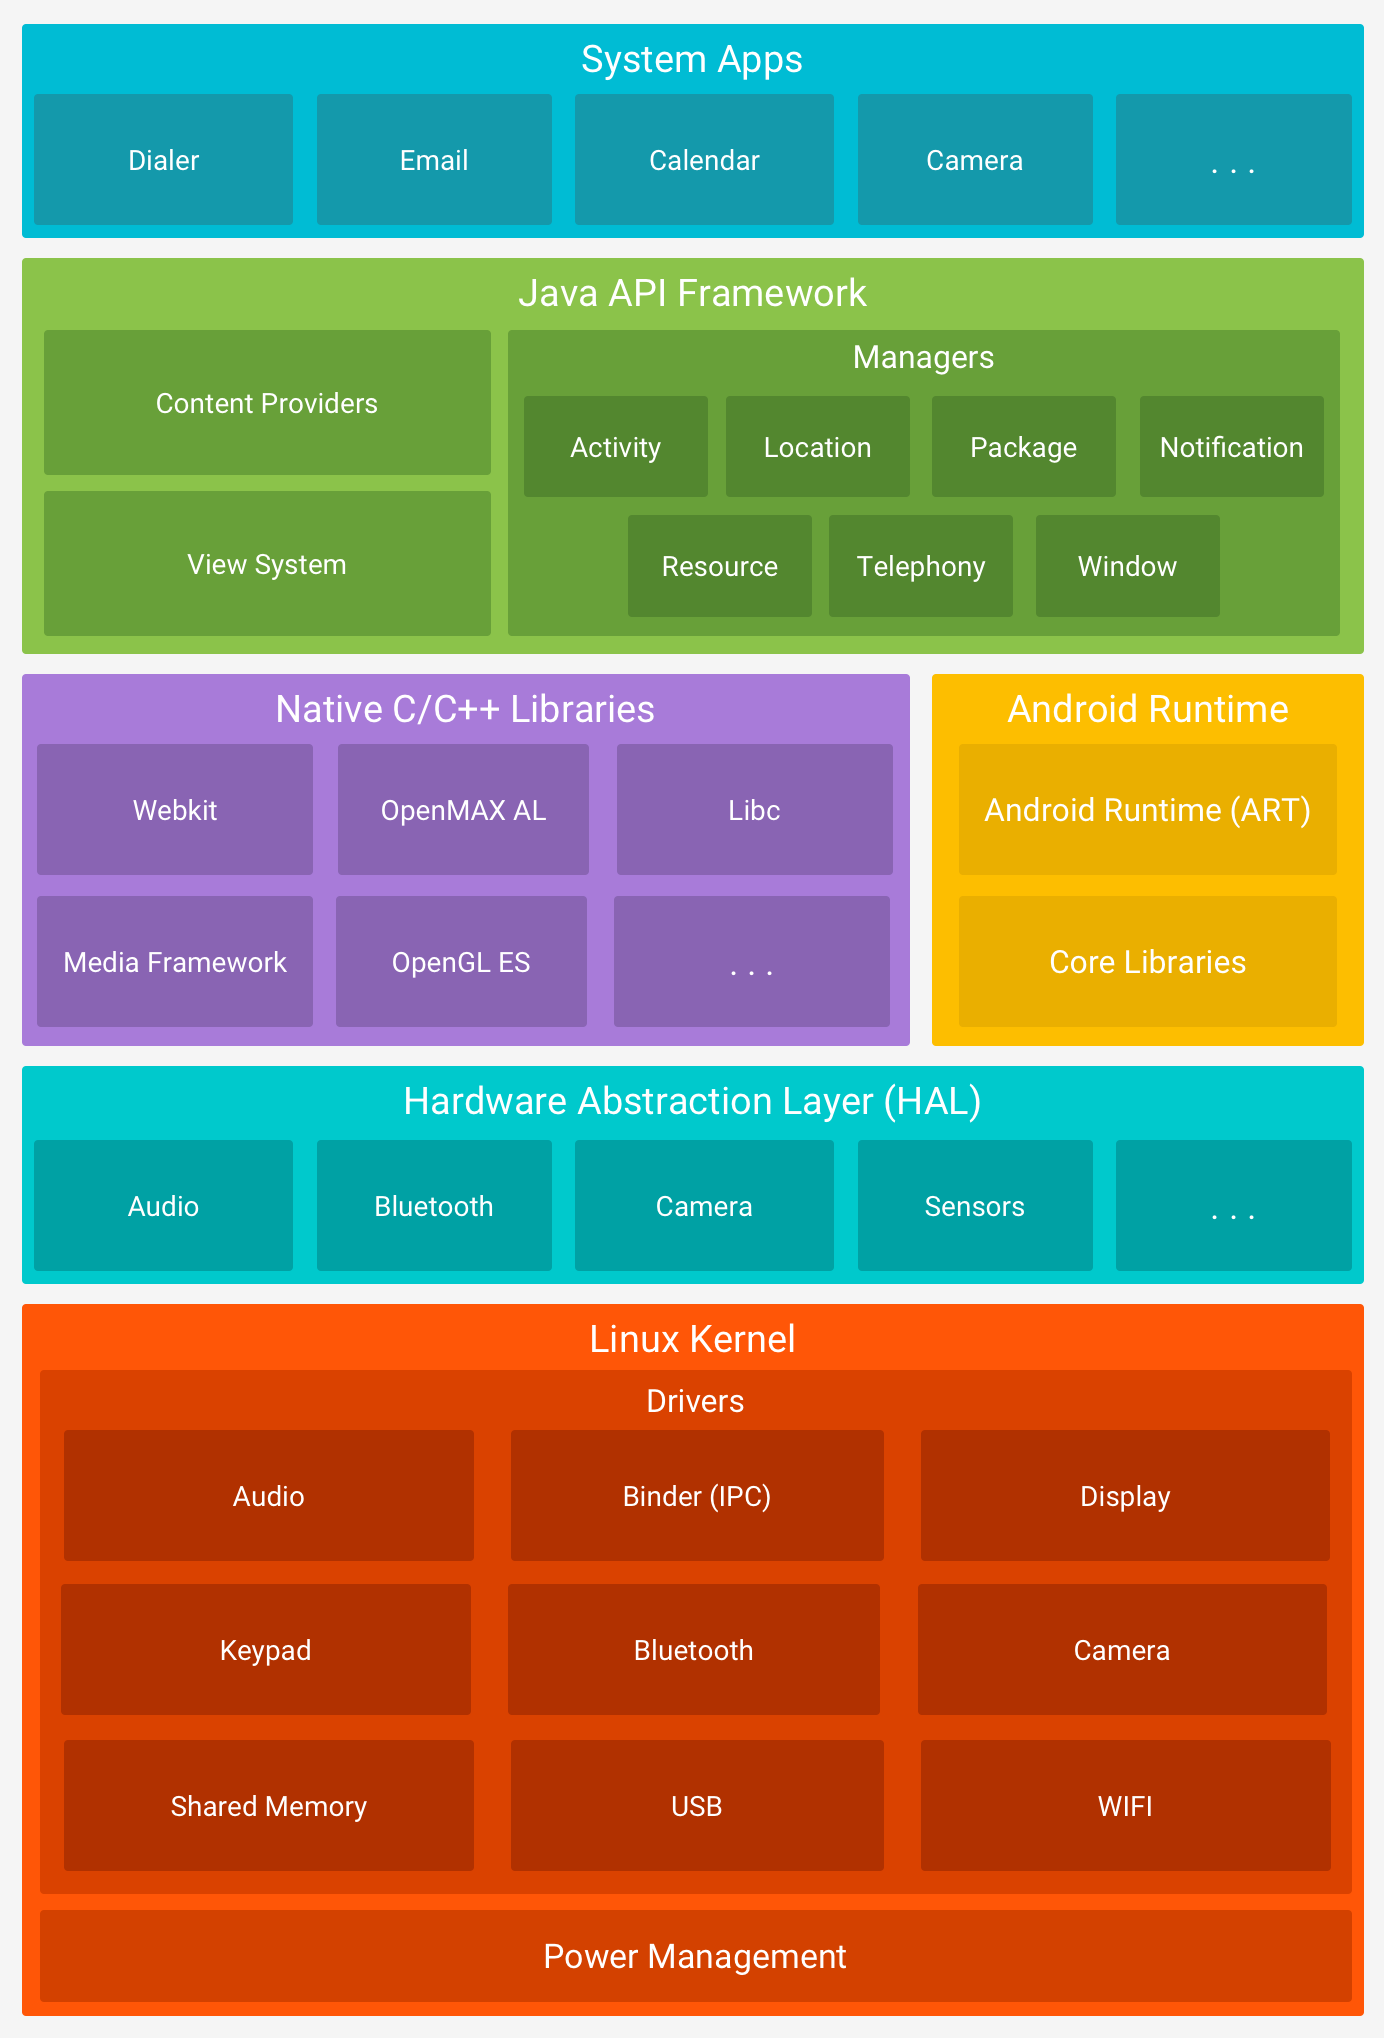
\includegraphics[width=100mm, keepaspectratio]{figures/android-stack_2x.png}
	\caption{Az Android operációs rendszer architektúrája.\cite{PlatformGuide}}
	\label{fig:AndroidPlatform}
\end{figure}

\subsection{Linux kernel}
Az operációs rendszer alapját a Linux kernel képezi, ezáltal ki tudja használni az évek során elért stabilitást és biztonságot, illetve lehetővé teszi a készülékgyártóknak, hogy egy már jól ismert technológiával dolgozzanak az illesztőprogramok fejlesztése során. Feladatai közé tartozik a memóriakezelés, a folyamatok ütemezése és a teljesítménykezelés. Ez utóbbi kiemelt fontosságú, hiszen a mobil eszközök akkumulátora véges, így a lehető legalacsonyabb fogyasztásra kell törekedni. \cite{MobWeb}

\subsection{Hardver absztrakciós réteg}
Közvetlenül a kernel felett található a hardver absztrakciós réteg - hardware abstraction layer, röviden HAL -, mely a készülék hardveres adottságait (pl.: kamera, szenzorok) ajánlja ki a felette található Java API keretrendszernek. Több modulból áll, melyek egy-egy specifikus hardverkomponens interfészt valósítanak meg, és a rendszer dinamikusan tölti be ezeket, amikor az API hozzá akar férni valamelyikhez. \cite{PlatformGuide}

\subsection{Android Runtime}
A következő komponens az Android Runtime, röviden ART. Ez egy virtuális gép, melyből mindegyik alkalmazás rendelkezik egy saját példánnyal, így egymástól és az operációs rendszertől izoláltan futhatnak. Mind az ART, mind az elődje, a Dalvik Virtual Machine specifikusan Androidra készültek. Az elődjéhez képest az Android Runtime rendelkezik plusz funkciókkal, ilyen többek között a telepítésidejű fordítás, az optimalizált szemétgyűjtés vagy a jobb hibakeresési támogatás. \cite{PlatformGuide}

\subsection{Natív C/C++ könyvtárak}
Ahogy azt a \refstruc{fig:AndroidPlatform} mutatja, natív C/C++ könyvtárak is helyet kaptak a rendszerben. Ezek a kernelen futnak, és sok rendszerkomponensnek szüksége van rájuk. A platform biztosít Java API-t néhányhoz, így például hozzáférhetünk az OpenGL grafikai könyvtárhoz natív kódból. \cite{PlatformGuide}

\subsection{Java API keretrendszer}
A fejlesztők számára a legfontosabb elem a Java API keretrendszer. Ez tartalmazza az operációs rendszer minden funkcióját, a moduláris, könnyedén újrahasznosítható építőelemeket, melyek felhasználásával a fejlesztők alkalmazásaikat elkészíthetik. Többek között magában foglalja az alábbiakat:
\begin{itemize}
	\item \emph{View System:} Felhasználói felületek létrehozásában van segítségünkre, kiterjedt és még tovább bővíthető elemkészlettel (pl.: listák, szövegmezők, gombok).
	\item \emph{Resource Manager:} Hozzáférést biztosít a fejlesztőnek minden erőforrásfájlhoz. Ezek tipikusan XML-fájlok, melyek leírják a projektben használatos lokalizált szövegeket, vektorgrafikus ábrákat és a fentebb is említett felhasználói felületeket.
	\item \emph{Activity Manager:} Az Android alkalmazások alapkövei az Activityk, melyeknek meghatározott életciklus-szakaszai vannak a létrehozástól a megszűnésig. Ezt az életciklust kezeli az Activity Manager, illetve egy közös navigációs backstacket biztosít, mely tárolja, hogy az alkalmazásban milyen képernyőket látogattunk meg a használat folyamán. \cite{PlatformGuide}
\end{itemize}

\subsection{Rendszeralkalmazások}
A rendszer beépített alkalmazásokkal érkezik a leggyakoribb feladatok elvégzésére. Ilyen például az SMS-küldés, internet böngészés, telefonálás, és a naptár. Ezek, ahogy a fenti bevezetőben is említettem, néhány kivételével teljesen lecserélhetők felhasználó által letöltött alkalmazásokra.

Mindez nem csak a felhasználó számára lényeges - a fejlesztő is fel tudja használni. Például, ha a fejlesztő szeretne telefonhívást indítani a saját alkalmazásából, akkor nem kell ezt a funkcionalitást implementálnia, elég csak meghívnia a készüléken elérhető alapértelmezett alkalmazást, ami majd elvégzi ezt. \cite{PlatformGuide}

\section{Fejlesztői környezet}

Az Android fejlesztés hivatalos eszköze az Android Studio, mely egy IntelliJ IDEA alapú integrált fejlesztési környezet, röviden IDE.\cite{AndroidStudio} Rengeteg funkcióval rendelkezik, így most csak a fontosabbakat fogom érinteni.

\subsection{Funkciók}
\begin{itemize}
	\item \emph{Build eszközök:} Rugalmas, Gradle-alapú build rendszert használ, így a projektbeállításokat és a külső könyvtárakat elég csak az erre kijelölt \emph{.gradle} kiterjesztésű fájlokba felvenni, a többit elvégzi helyettünk.
	\item \emph{Egységes környezet:} Nem kell külön program más eszközökre való fejlesztéshez, akár telefonra, táblagépre vagy okosórára szeretnénk alkalmazást írni, mindet megtehetjük a Studioból.
	\item \emph{Emulator:} Fejlesztésnél rendkívül praktikus, hogyha nem kell minden alkalommal fizikai készüléket keresni, ha futtatni szeretnénk a programunkat. Erre szolgál a beépített emulátor, amivel különböző virtuális készülékeken tesztelhetünk alkalmazásokat. Ez egy teljes operációs rendszert tár elénk, így nem csak az alkalmazásunkat tudjuk rajta megnézni, hanem a rendszeralkalmazások is mind elérhetők. Hívásindítást és -fogadást, SMS-eket, konfigurációváltozást vagy akár helyadat-változást is tudunk vele emulálni. Egyszerre több emulátorunk is lehet, ezeket az AVD Managerben tudjuk kezelni. Új létrehozásánál kiválaszthatjuk, hogy milyen készülékmodellt szeretnénk, melyik Android verzióval, és egyéb hardverbeállításokat is megadhatunk, például, hogy mennyi memóriát szeretnénk a készüléknek.
	\item \emph{Verziókezelés:} Az IDE több verziókezelő rendszert is beépítetten támogat, így egy kényelmes felületen intézhetjük a változtatások követését.
	\item \emph{Kódelemzési funkciók:} Ezek azok, amik igazán kényelmessé teszik az Android Studio használatát. Folyamatos segítséget nyújt a kódírásban, a kódkiegészítés jelentősen meggyorsítja a haladást. Jelzi, ha bármi elavult, így nem utólag kell megváltoztatni a kódot. Az egyik leghasznosabb funkció pedig a nem használt kódrészletek jelzése. Mivel az IDE kiszürkíti azokat a változókat és függvényeket, amik egyszer sincsenek meghívva, így könnyű karbantartani, hogy ne maradjon a kódbázisban felesleges sor.
\end{itemize}

\subsection{Projektstruktúra}
Minden projekt egy vagy több modulból áll, és mindent tartalmaz a forráskódtól kezdve a tesztkódon át a build konfigurációkig. A modulok segítségével különálló funkcionalitási egységekre bontható az alkalmazás, melyeket egymástól függetlenül lehet buildelni, tesztelni és debugolni. \cite{ProjectStructure}
Célszerű modulokat használni, ha például különböző eszköztípusokra szeretnénk fejleszteni, hiszen így az egymástól független részeket elkülöníthetjük, de a közös kódot meg tudjuk osztani köztük.

A fejlesztőkörnyezetet megnyitva a projektfájlok megjelenítése alapértelmezetten eltér a fájlrendszerbeli hierarchiától. Ezt Android nézetnek hívja az IDE, és úgy lett kifejlesztve, hogy a lehető legkényelmesebb legyen a fejlesztők számára. Itt alapvetően három mappára szedve találhatók meg a forrásfájlok.

Az első a \emph{manifests}, melyben az \emph{AndroidManifest.xml} fájl található. Ez fontos adatokat tartalmaz az alkalmazásról, melyekre szüksége van a build eszközöknek, az operációs rendszernek, és a Google Play-nek is. Fel kell sorolni benne többek között az összes komponensét, a futás során szükséges engedélyeket (pl.: fájlrendszer-hozzáférés, kamera), illetve a működéshez elengedhetetlen szoftveres és hardveres funkciókat. Utóbbit ellenőrzi is a Play Store, és csak olyan készülékekre engedi feltelepíteni az alkalmazást, melyek ennek megfelelnek. \cite{Manifest}

A következő mappa általában \emph{java} névre hallgat, és ebben található a projekt összes forráskódja. A nevével ellentétben ma már legtöbbször Kotlin kódot tartalmaz, mivel 2019 óta ez az Android fejlesztés hivatalos, preferált nyelve, de az elnevezés megmaradt azokból az időkből, amikor még mindenki Java-t használt.

Az utolsó mappa pedig a \emph{res}, melyben az erőforrásfájlok találhatók. Ezek általában XML fájlok, és az alkalmazásban felhasznált layoutokat, animációkat, stringeket írják le, de ide kerülnek például a képi erőforrások is.

%------------------------------
\chapter{Architektúra}
%------------------------------

A fejlesztés során elsődleges célom volt, hogy egy olyan architektúrára alapozzam az alkalmazást, mely megfelelően szétválasztja a felelősségeket, és ezáltal egy könnyen karbantartható, átlátható kódot alkossak. Először egyből az MVVM (Model - View - ViewModel) architektúrára gondoltam, mivel azt már korábban is használtam, és jó tapasztalataim voltak vele. A RainbowCake\cite{Rainbowcake} egy MVVM-re építő architektúra, melynek fő fókusza a felelősségek szétválasztása és a képernyő konzisztens állapotban tartása. Tekintve, hogy ez pontosan megegyezik a céljaimmal, így a kipróbálása mellett döntöttem.

\section{Felépítés}

Az architektúra rétegeit a \refstruc{fig:RainbowCakeLayers} szemlélteti.

\begin{figure}[!ht]
	\centering
	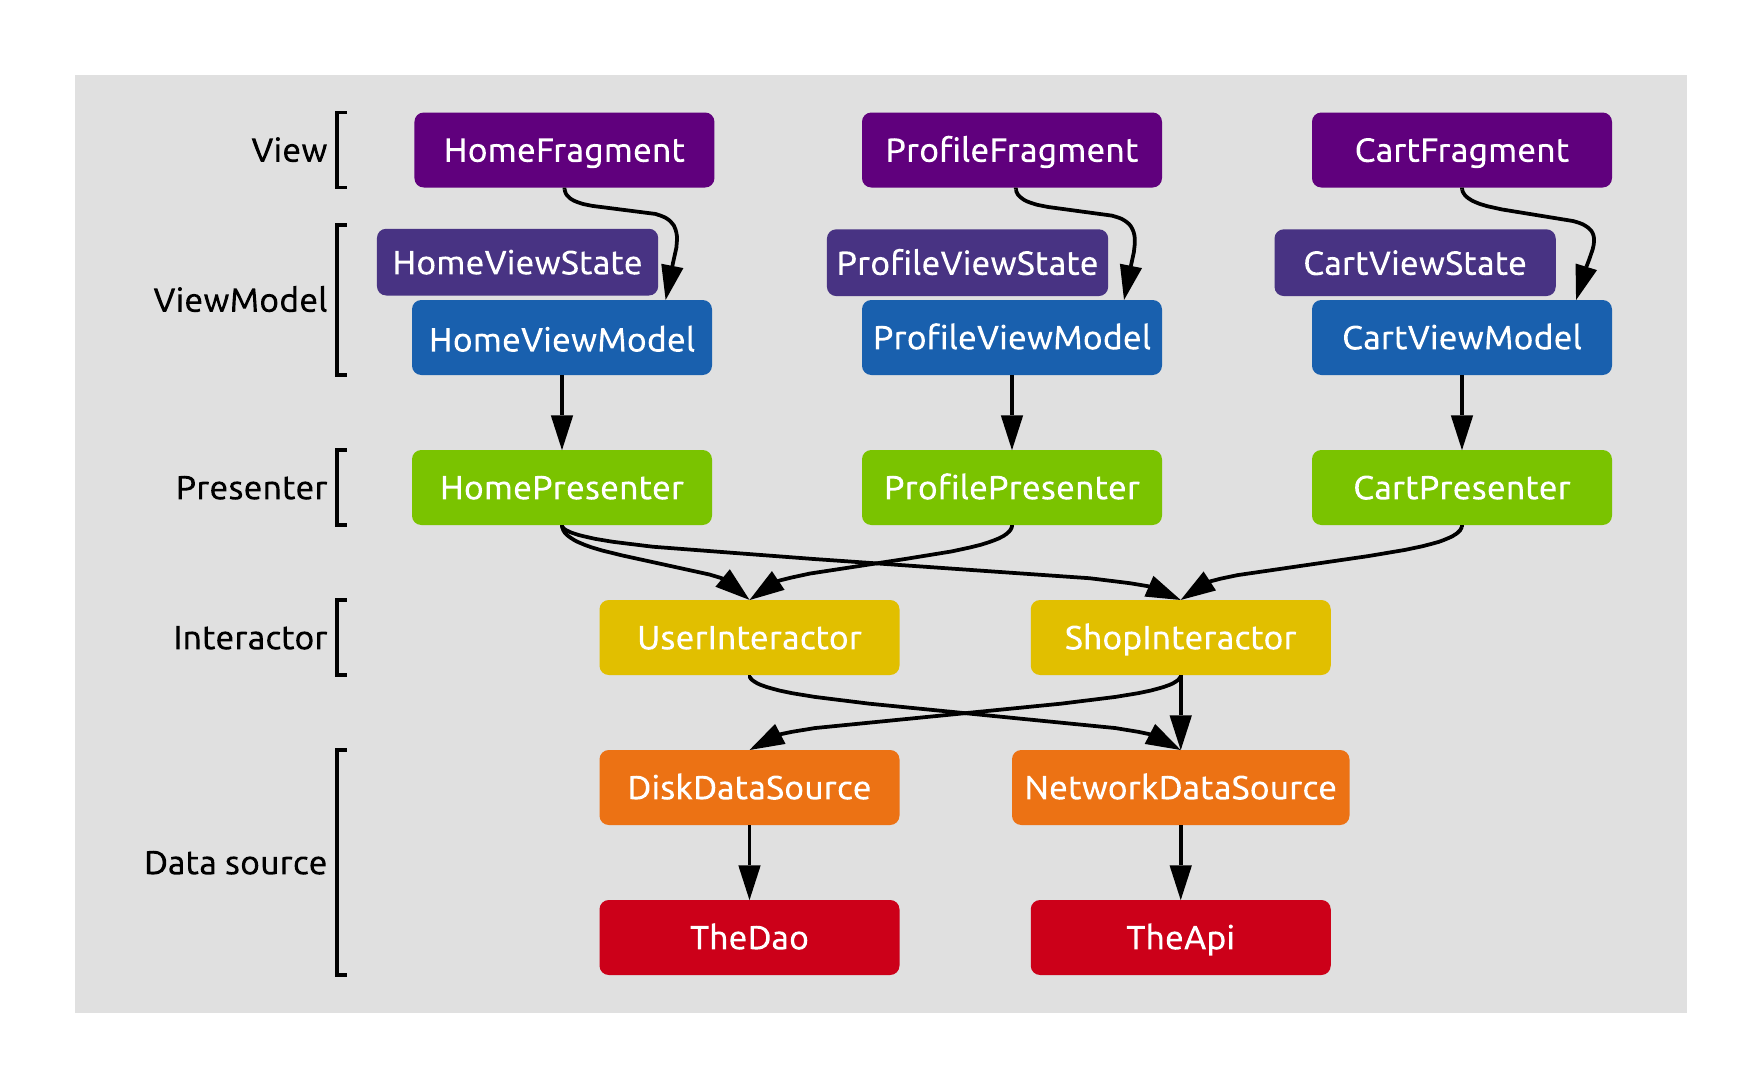
\includegraphics[width=150mm, keepaspectratio]{figures/final-architecture.png}
	\caption{A RainbowCake architektúra rétegei.}
	\label{fig:RainbowCakeLayers}
\end{figure}

\subsection{View}
A view-k alkotják az alkalmazás képernyőit, melyekkel a felhasználó találkozik használat közben. Ezek lehetnek Activityk vagy Fragmentek, és fő feladatuk továbbítani a felhasználói inputot a ViewModel felé, melytől cserébe új adatot, állapotot vagy eseményt kapnak. 

\subsection{ViewModel}
A felhasználói felülettel kapcsolatos logikát végzik, illetve tárolják és a Presentertől kapott adatok alapján frissítik a képernyőhöz tartozó ViewState-et.

\subsection{Presenter}
Háttérszálra teszik a hívásokat, és továbbítják azokat az Interactorok felé, majd az eredményt képernyő specifikus prezentációs modellekké transzformálják, és azt adják oda a ViewModelnek. A projektből ezt a réteget teljesen kihagytam, mivel a View ugyanazt a modellt jeleníti meg, mint amit az adatbázisból visszakap, így nem volt szükség a modelltranszformációra.

\subsection{Interactor}
Az Interactorok, ahogy az ábrán is látható, nem egy-egy képernyőhöz köthetők, hanem funkcionalitásokhoz. Ők végzik a fő üzleti logikát, manipulálják az adatokat és számításokat végeznek. Az alkalmazásomban csak egyetlen darab van, ugyanis az adatok megjelenítése nem igényel sok üzleti logikát, viszont Presenterek hiányában ő kapta meg a felelősséget, hogy a hívásokat háttérszálra tegye. 

\subsection{DataSource}
Egységes interfészt biztosítanak az adathozzáféréshez, feladatuk a különböző hívások (pl.: lokális adatbázis, Firebase) implementációjának elfedése, és az adatok konzisztens állapotban tartása. 

\section{Funkciók}

A következőkben röviden kifejtem az architektúra főbb funkcióit, melyek segítségemre voltak az alkalmazás fejlesztése során. 

\subsection{Dependency Injection}
A függőséginjektálás - dependency injection, röviden DI - egy gyakran használt technika, mely jelentősen könnyebbé teszi a kód újrafelhasználását, refaktorálását és tesztelését.\cite{DepInjection}

Függőségnek nevezzük azt, amikor egy osztálynak szüksége van egy másik osztály működésére vagy képességeire. Ilyenkor, ha ezt saját maga példányosítja, akkor szoros csatolás jön létre a két osztály között, ennek következményeképpen pedig nem lehet a tartalmazott objektum helyett később egy másik implementációt vagy leszármazottat használni. Emellett a tesztelés is megnehezedik, hiszen az osztály egy valódi példányt használ a másikból, azt nem tudjuk egy tesztobjektummal helyettesíteni.

Függőséginjektálásról akkor beszélünk, hogyha a fent leírt módszer helyett az osztály a függőségeit paraméterként kapja, például a konstruktorban. Ezáltal az említett problémák megszűnnek, az osztályunk újrafelhasználható lesz, és könnyedén tesztelni is tudjuk, ha valós függőség helyett egy mock objektumot adunk neki. 

A DI megvalósítására két opció létezik: manuális, illetve automatizált. Az előbbi kisebb alkalmazásoknál megoldható lehet, ha csak pár osztály létezik kevés függőséggel, de nagyon hamar kezelhetetlenné válik az alkalmazás növekedésével. Erre nyújtanak megoldást a különböző könyvtárak, melyek megfelelő beállítások mellett automatikusan elvégzik a függőségek létrehozását és biztosítását. 
Egy ilyen könyvtár a Dagger 2, mely az egyik legnépszerűbb ezen a téren. A RainbowCake beépítetten támogatja a használatát, csak a megfelelő függőségeket kell felvenni a projektbe. Ezt követően még pár beállítást el kell végeznünk a projekten, majd az injektálni kívánt konstruktorokat \emph{@Inject} annotációval megjelölni, a többit pedig elvégzi helyettünk.

%TODO a "pár beállítást" szerintem nyugodtan fejts ki
%TODO nem konstruktort akarunk injektálni, hanem a konstruktorban átadaott paramétereket injektáljuk. szóval egy picit átfogalmazás kellene ide
%TODO a többiet elvégzi helyettünk kicsit flegma, ha ki tudnád fejteni, hogy mit tud megoldani, vagy milyen esetekre használtad, jól jönne

\subsection{View State}
A RainbowCake állapotkezelése jelentősen megkönnyíti a UI különböző állapotainak nyomon követését, és az annak megfelelő nézet megjelenítését. Ha egy képernyőnek több egymástól független, elkülöníthető állapota van, akkor ezt nem érdemes egyetlen \emph{data class} tagváltozóiban tárolni, mert az inkonzisztens állapothoz vezethet.\cite{ViewState} 

Erre kínál egy kényelmes megoldást a Kotlinban elérhető \emph{sealed class}, mely egy olyan osztály, aminek fordítási időben ismerjük az összes leszármazottját. Ha a fragment állapotait egy ilyen \emph{sealed class}-ból származtatjuk le, akkor lévén osztályok, tartalmazhatnak saját tagváltozókat (például a megjelenítendő adatokat vagy a hibaüzenetet), és a Kotlin \emph{when} feltételes szerkezetének segítségével ki lehet kényszeríteni, hogy minden állapot le legyen kezelve. Így már nem fordulhat elő inkonzisztencia, hiszen az egymást kölcsönösen kizáró állapotokból egyszerre csak egy lehet aktív a futás során. A képernyő render logikája pedig leegyszerűsödik: az architektúra által biztosított \emph{render} függvényben az állapottól függően változtathatjuk a megjelenítést. Az pedig garantálva van, hogy a \emph{render} mindig lefut, amikor megváltozik a képernyő állapota.

\subsection{ViewFlipper}
A ViewFlipper egy layout komponens, mely az állapotok olvasható elkülönítését teszi lehetővé. \cite{ViewFlipper} Ugyanis, ha a képernyő minden elemét külön manipuláljuk a fent említett \emph{render} függvényben, akkor ez egy idő után olvashatatlan kódot fog eredményezni, rengeteg hibalehetőséggel. Ezt orvosolja a ViewFlipper, melyben egyszerre egy tartalmazott layoutot tudunk megjeleníteni, így nem kell manuálisan állítani a különálló elemek láthatóságát. Használata rendkívül egyszerű, a layoutot leíró XML fájlban egy ViewFlipper komponenst kell létrehozni (\refstruc{fig:ViewFlipperComponent}), az épp látható gyerek elemét pedig a \emph{displayedChild} tagváltozón keresztül tudjuk elérni és módosítani (\refstruc{fig:ViewFlipperUsage}).

\begin{figure}[!ht]
	\centering
	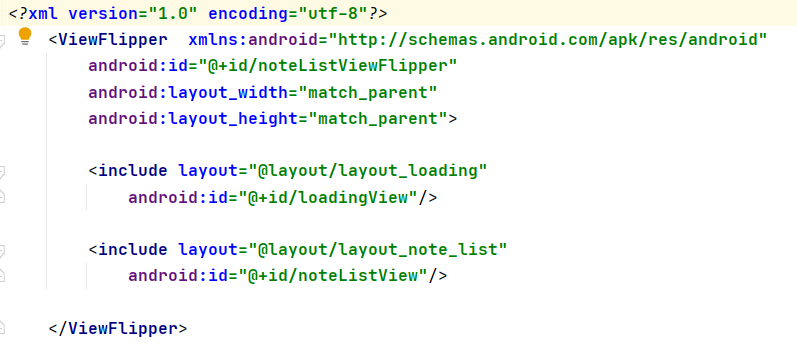
\includegraphics[width=150mm, keepaspectratio]{figures/view_flipper_impl.png}
	\caption{A ViewFlipper komponens használata XML-ben.}
	\label{fig:ViewFlipperComponent}
\end{figure}

\begin{figure}[!ht]
	\centering
	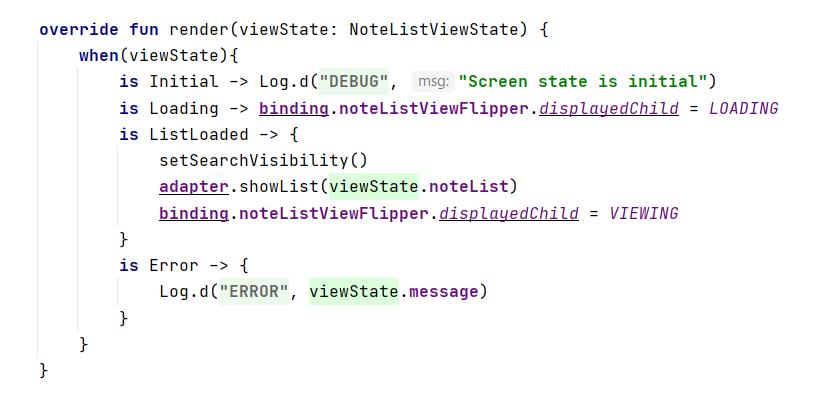
\includegraphics[width=150mm, keepaspectratio]{figures/view_flipper_usage.png}
	\caption{A ViewFlipper megjelenített gyerekének változtatása.}
	\label{fig:ViewFlipperUsage}
\end{figure}

\subsection{Események}
A RainbowCake biztosít keretet arra is, hogyha egyszeri eseményeket szeretnénk a képernyőn megjeleníteni. Ilyen lehet például, ha hibába ütközik az alkalmazás, vagy a visszakapott adatok alapján navigálni szeretnénk egy másik képernyőre. Ezt nem tárolhatjuk az állapotban - hiszen nem olyan dolog, ami minden renderelésnél történik -, ezért megalkották a \emph{OneShotEvent} típust, mely az ilyen eseményeket reprezentálja. \cite{Events}

Használata rendkívül egyszerű, minden lehetséges event típust definiálunk a ViewModelben, majd a megfelelő helyeken a \emph{postEvent} függvénnyel tudjuk elküldeni a fragmentnek, mely az \emph{onEvent} függvény felüldefiniálásával tudja ezeket kezelni. 

\subsection{Tesztelés}
A könyvtár tartalmaz beépített támogatást a ViewModelek és a Presenterek tesztelésére, ezek közül a projekt szempontjából a ViewModel tesztelése releváns. Ennek a fő nehézségét az adja, hogy a beérkezett adatokra állapotváltozás, illetve események formájában reagál a ViewModel, melyeket a validáláshoz meg kell figyelnünk valamilyen módon. \cite{RainbowcakeTest}

Ehhez nyújt segítséget az architektúra \emph{ViewModelTest} osztálya. A tesztosztályunkat ebből leszármaztatva elérhetővé válik a \emph{observeStateAndEvents} függvény, mely biztosít egy \emph{stateObserver} és egy \emph{eventsObserver} objektumot. Az előbbi a teszt futása során előforduló \emph{ViewState}-eket figyeli, az utóbbi pedig az eseményeket. Mindkét \emph{observer} tartalmaz \emph{assert} függvényeket az eredmények ellenőrzésére, ilyen például az \emph{assertObserved}, amivel a futás során előforduló összes állapotot vagy eseményt hasonlíthatjuk az elvárthoz, illetve az \emph{assertObservedLast}, mely az előzővel ellentétben csak a legutolsót figyeli.

%--------------------
\chapter{Felhasznált könyvtárak}
%--------------------
%TODO write
%TODO intro

\section{Google Cloud Vision API}

A Vision API a Google Cloud szolgáltatásainak képfelismerésre specializált része. Használata csak egy bizonyos, havonta újuló kvótáig ingyenes, mely szerencsére bőven elegendő volt a projekt elkészítése és tesztelése során. Számos előre betanított modellt tartalmaz, melyekkel detektálhatunk és osztályozhatunk tárgyakat, arcokat, szövegeket vagy akár felnőtt tartalmakat is. \cite{Vision}

A jegyzetek digitalizálásához szövegfelismerésre van szükség, ami optikai karakterfelismerés alkalmazásával valósítható meg. Ez az API \emph{DOCUMENT\_TEXT\_DETECTION} funkciójával lehetséges, mely optimalizálva van mind nagy sűrűségű dokumentumok, mind kézírás detektálására. Ennek során a kiválasztott képet egy base64 kódolt string formájában kell az API-nak elküldeni, a kívánt felismerés elvégzése után pedig az eredményt egy \emph{TextAnnotation} típusú objektumban kapjuk vissza. Ez egy strukturált reprezentációja a kinyert szövegnek, amit oldalakra, paragrafusokra vagy akár szavakra is bonthatunk. A projekt esetében elegendő volt az objektumon a \emph{text} property használata, mely az eredményt egyetlen stringben adja vissza. 

A szolgáltatás számtalan nyelvet támogat, többek között a magyart is, és végül emiatt esett erre a választásom. Nincs is igazán sok elérhető API, mely képes lenne kézírás-felismerésre, de ez az egyetlen ami ezt magyarul is támogatja. Esetleg a Microsoft Azure Computer Vision szállhatna vele versenybe, de ilyen téren az is elmarad, mert jelenleg csak nyomtatott dokumentumok detektálására képes magyarul. Kerestem más alternatívákat is, de a legtöbb kézírás-felismerő szolgáltatás a digitális jegyzetelésre koncentrál - amikor a felhasználó egy érintőképernyőre ír egy speciálisan erre készített "tollal" -, de nekem a use case-t tekintve ezek nem feleltek meg.

Az API kézírás-felismerő képességének megvannak a korlátai, amik kevésbé használhatóvá teszik az alkalmazást, mint amennyire én terveztem. Ma már az Egyesült Államokban elég ritkán írnak kézzel az emberek, és ez meglátszik a modell teljesítményén. Az én kézírásom szinte megfejthetetlen a Vision API számára, nagyon gondosan és odafigyelve kell formálnom a betűket ahhoz, hogy felismerje. A szép kézírást viszont egészen megbízhatóan teljesíti, illetve az írott nagybetűkkel is elboldogul. Így sajnos nem sikerült egy olyan szinten használható alkalmazást készíteni belőle, mint ahogy én elképzeltem, de szebben írt, rövidebb szövegek digitalizálására tökéletesen megfelel. 

\section{Firebase}

A Firebase szintén a Google terméke fejlesztők számára, mely megkönnyíti és felgyorsítja a fejlesztési folyamatokat azáltal, hogy egy teljes backend-infrastruktúrát biztosít. Így a fejlesztőnek elég csak ezeket a szolgáltatásokat integrálnia az alkalmazásába ahelyett, hogy azt is külön írnia kellene. Lehetőséget kínál felhasználó-kezelésre, adattárolásra, teljesítményfigyelésre, biztosít analitikát, crash-elemzést és még sok mást. 

Alább találhatók azon Firebase-szolgáltatások, melyeket felhasználtam az applikáció fejlesztése során; most ezekre fogok kicsit bővebben kitérni.

\subsection{Cloud Firestore}
Egy alkalmazásban a felhasználó által bevitt adatokat valamilyen módon el kell tárolnunk, hogy aztán később is hozzá lehessen férni. Erre két lehetőségünk van: lokális adatbázis használata a készüléken (pl.: Room) vagy a felhőalapú adattárolás. Én az utóbbit választottam, mert felhasználói szempontból sokkal kényelmesebb egyszer egy fiókot csinálni és ahhoz kötni az adatokat, mint mondjuk egy esetleges készülékcserénél kutatni, hogy hogyan lehet átemelni az adatokat az újra. A Firebase két szolgáltatást is biztosít erre a célra, ezek név szerint a Realtime Database és a Cloud Firestore. 

A Realtime Database régebb óta létezik, és az adatok JSON formátumú tárolására ad lehetőséget. Ez egyszerű adatszerkezet esetén ideális, de a komplex, hierarchikus adatok szervezésére nem a legjobb választás. Ezen okból döntöttem inkább a Cloud Firestore használata mellett. 

A Cloud Firestore a Firebase legújabb adatbázis-szolgáltatása, mely egy új, intuitívabb adatmodellre épít gyorsabb lekérdezésekkel és jobb skálázódással. \cite{RealtimevsFirestore} Adatmodelljét tekintve egy NoSQL adatbázisról van szó, melyben táblák és sorok helyett dokumentumokba és kollekciókba rendezve tároljuk az adatot. A dokumentumok kulcs-érték párokból állnak, de tartalmazhatnak kollekciókat is, melyekben további dokumentumok találhatók. \cite{FirestoreDataModel} Az adatbázisnak nincs sémája, így szabadon alkothatjuk meg az adataink struktúráját - akár ugyanazon a kollekción belül található két dokumentum tartalma is eltérhet egymástól. 

Emellett a Firestore biztosít még egy rugalmas szabályrendszert, melynek segítségével kontrollálhatjuk a hozzáférést az adatbázisunk különböző részeihez. Itt úgynevezett \emph{match} kifejezésekkel illesztjük rá a szabályokat a megadott elérési útvonalakra, és ha a szabályok nem teljesülnek akkor a lekérdezés meghiúsul. Különböző szabályokat adhatunk meg olvasásra és írásra, de akár lebontva a \emph{get, list, create, update, delete} műveletekre is. 

Az applikáció biztonsági szabályai a következőképpen néznek ki (\refstruc{fig:FirestoreRules}).

\begin{figure}[!ht]
	\centering
	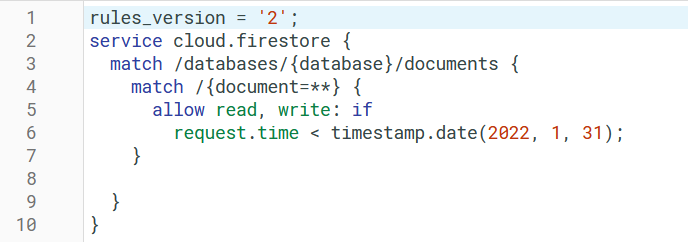
\includegraphics[width=120mm, keepaspectratio]{figures/rules.png}
	\caption{A projekt biztonsági szabályai.}
	\label{fig:FirestoreRules}
\end{figure}

A fenti szabály minden dokumentumra illeszkedik, és megenged minden írást és minden olvasást abban az esetben, hogyha a lekérdezés 2022. január 31. előtt érkezik be. Ez egy tesztszabály, melyet a Firestore generál a projekt létrehozásakor a fejlesztés megkönnyítése céljából. Természetesen ezt éles alkalmazásban mindenképpen le kell cserélni, hiszen így bárki hozzáférhet az adatbázishoz, aki tudja a projektazonosítót, ám a tesztelési fázisban még bőven elegendő.

\subsection{Autentikáció}
Ahhoz, hogy a felhasználók csak és kizárólag a saját adataikhoz férjenek hozzá, valamilyen módon tárolni és azonosítani kell őket. Erre kínál megoldást a Firebase Authentication, mely backend-szolgáltatásokat, könnyen használható SDK-kat és UI könyvtárakat biztosít a felhasználók autentikációjára. Lehetővé tesz többek között jelszavas, telefonszámos, illetve harmadik fél általi (pl.: Google, Facebook, Twitter) bejelentkezést is. Automatikusan integrálódik más Firebase szolgáltatásokkal, de saját fejlesztésű háttérrendszerekkel is könnyedén használható.  \cite{Auth}  

\subsection{Analytics}
A Firebase Analytics egy ingyenes analitikai megoldás, mely szintén integrálódik más Firebase szolgáltatásokkal. Automatikusan elkap előre definiált eseményeket, de lehetővé teszi a fejlesztő számára saját események létrehozását. Az aktivitást, és a megfigyelt események alapján alkotott statisztikákat pedig bejelentkezés után el lehet érni a Firebase console\footnote{\url{https://console.firebase.google.com}}-ban az alkalmazás adatai alatt. \cite{Analytics} Számos hasznos metrikát és diagramot készít az applikáció stabilitásáról, használatáról vagy éppen bevételéről. A fejlesztő figyelemmel kísérheti, hogy hányan használják az alkalmazást (\refstruc{fig:AnalyticsPlatform}), mely országokból (\refstruc{fig:AnalyticsCountries}), illetve információt kaphat a tevékenységek időtartamáról, platformokról és elkapott eseményekről. 

\begin{figure}[!ht]
	\centering
	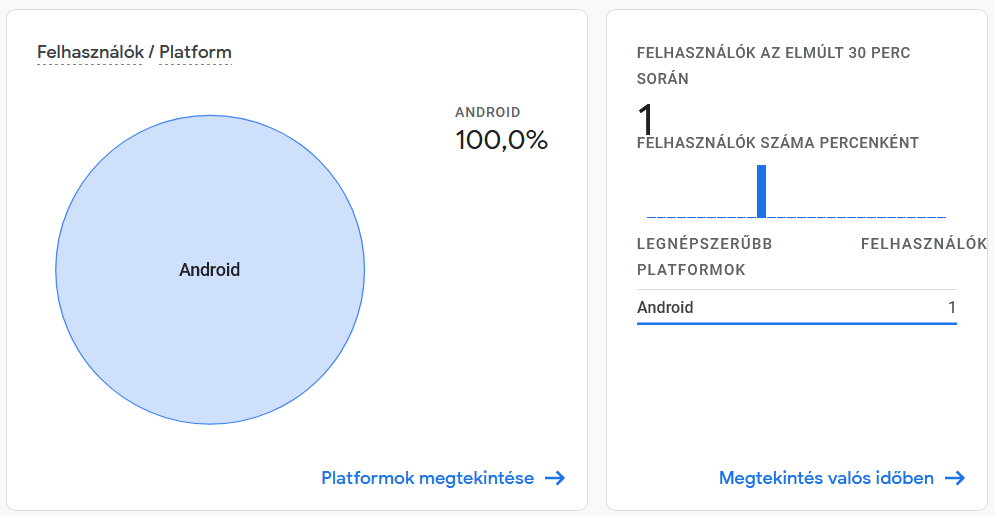
\includegraphics[width=150mm, keepaspectratio]{figures/analytics_platform.png}
	\caption{Platform megoszlása a felhasználók között, közelmúlt aktivitása.}
	\label{fig:AnalyticsPlatform}
\end{figure}

\begin{figure}[!ht]
	\centering
	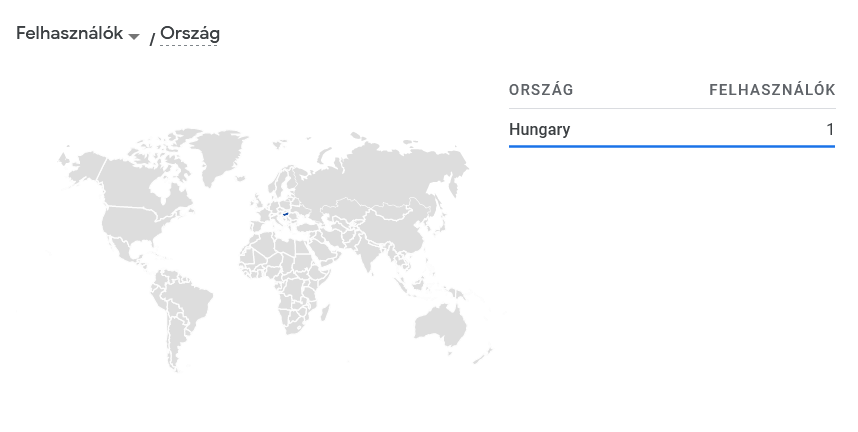
\includegraphics[width=150mm, keepaspectratio]{figures/analytics_countries.png}
	\caption{Felhasználók megoszlása az országok között.}
	\label{fig:AnalyticsCountries}
\end{figure}

Ezen statisztikák nyilvánvalóan nem annyira látványosak ilyen kis mértékű felhasználással, de egy nagyobb felhasználóbázisnál már jelentősen segíthetik az alkalmazás fejlődését. Mindez nem csak a fejlesztőknek lényeges, hanem az üzleti résztvevőknek is, hiszen az Analytics számos statisztikát készít a bevételekről és az ügyfélszerzésről is. 

\subsection{Crashlytics}
A Firebase Crashlytics jelentéseket készít a fejlesztőknek a felhasználókat érő crashekről. Segít nyomon követni és priorizálni a hibákat, csoportosítja őket, és kiemeli a hozzájuk vezető körülményeket. Valósidejű figyelmeztetést küld az újonnan felbukkanó vagy éppen növekvő problémákról, melyek azonnali figyelmet igényelhetnek. \cite{Crashlytics} 

Szintén a Firebase console-ban érhető el, ahol láthatjuk a crash-free statisztikát (\refstruc{fig:CrashlyticsCrashfree}), a trendeket és az aktuális problémákat. Utóbbira kattintva még bővebb információt kaphatunk az előfordulási gyakoriságról, az érintett felhasználókról és verziókról, és a crash teljes stack trace-ét megtekinthetjük, kiemelve a keletkezés helyét és okát. 

\begin{figure}[!ht]
	\centering
	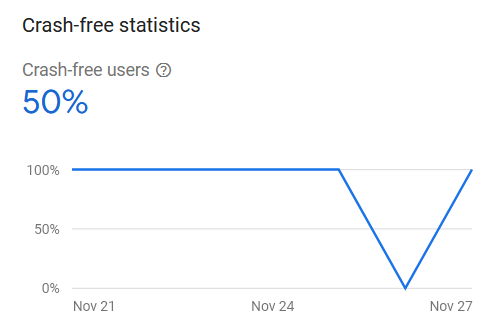
\includegraphics[width=110mm, keepaspectratio]{figures/crashlytics_crashfree.png}
	\caption{Crash-free felhasználók aránya napokra lebontva.}
	\label{fig:CrashlyticsCrashfree}
\end{figure}

\section{Groupie}

Android alkalmazásokban szinte mindig található legalább egy darab listanézet, mely ugyanolyan típusú elemeket sorol fel a képernyőn. Ezt legegyszerűbben a \emph{RecyclerView} komponens segítségével lehet megoldani, mely a megvalósítás mélységeit elfedi előlünk. Két dolgot kell megadnunk a működéséhez: egy sor kinézetét, illetve a megjelenítendő adatokat. A RecyclerView - ahogy a neve is sejteti - újrahasznosítja a lista elemeit, ami annyit jelent, hogy a képernyőről eltűnő sorokat nem megszünteti, hanem azokat használja fel az éppen megjelenő sorok létrehozásakor. Mindez jelentősen javítja az alkalmazás teljesítményét és csökkenti az energiafelhasználást. \cite{RecyclerView}

Azonban a projekt során szükségem volt egy funkcióra, amit a RecyclerView alapértelmezetten nem tud, ez pedig a lista elemeinek kinyitható/becsukható csoportokba szervezése. Így találtam rá a Groupie névre hallgató könyvtárra, mely kiküszöböli ezt a hiányosságot. 

A Groupie nagyban megkönnyíti a listák kezelését, ugyanis a tartalmat logikai csoportokként kezeli. \cite{Groupie} Használata rendkívül egyszerű: mindenhol, ahol eddig \emph{RecyclerView.Adapter}-t kellett használni, ezután \emph{GroupieAdapter} szerepel majd. Minden típusú megjeleníteni kívánt elemnek készíteni kell egy saját osztályt, mely a könyvtár által biztosított \emph{Item} osztályból származik le, és felparaméterezi a neki szánt layout-ot a kapott adatokkal. A speciális viselkedések támogatására léteznek különféle interfészek, melyeket pluszban megvalósíthatunk a kívánt működés elérése érdekében. Ilyen például az \emph{ExpandableItem}, mely pontosan azt a funkcionalitást biztosítja, amire szükségem volt: rendelhetők alá egyéb elemek, melyek felhasználói interakció hatására elrejthetők illetve megjeleníthetők. 

A listák építőelemei itt a csoportok, ahol egy item egyelemű csoportnak számít. Így leegyszerűsödik a lista feltöltése is, ugyanis akár felváltva adhatunk az adapterhez többelemű csoportokat és egyes elemeket. Automatikusan kezeli a lista tartalmának változását, így nem kell manuálisan ezzel foglalkozni és csökken a hibalehetőségek száma. Emellett nagy hangsúlyt fektettek a bővíthetőségre, a könyvtár tudatosan úgy lett felépítve, hogy a lehető legegyszerűbb legyen a meglévő osztályok felhasználásával saját viselkedést definiálni. Ez pedig egy hatalmas előny, ami az enyémnél sokkal komplexebb use case-ekre is alkalmassá teszi. 

\section{EasyPermissions}

Android platformon a felhasználó adatait és készülékét egy komplex engedélyrendszer védi. Az operációs rendszer \emph{Marshmallow} névre hallgató verziója (6.0) előtt minden engedélyt telepítési időben kellett jóváhagyni, ám idővel kiderült, hogy ez nem nyújt megfelelő védelmet, hiszen a felhasználók nem olvassák el telepítés előtt, hogy mibe egyeznek bele. Ezért született meg a ma is használatos rendszer, melyben az engedélyek három csoportba sorolhatók:
\begin{itemize}
	\item \emph{Telepítésidejű engedélyek:} Ezek korlátozott hozzáférést biztosítanak olyan adatokhoz és tevékenységekhez, melyek minimálisan befolyásolják a rendszert, és az alkalmazás telepítésével megadásra kerülnek. Ilyen például a hozzáférés a hálózathoz, internethez vagy épp a rezgőmotorhoz. Két típusba sorolhatók: lehetnek normál engedélyek, amik csak nagyon kis kockázatot jelentenek a felhasználó adataira és más alkalmazások működésére, illetve \emph{signature} engedélyek, melyek akkor kerülnek telepítéskor elfogadásra, ha egy már korábban a készülékre telepített alkalmazás elkérte az adott engedélyt, és ugyanaz a tanúsítvány írja alá ezt és a telepítendő applikációt. 
	\item \emph{Futásidejű engedélyek:} További hozzáférést biztosítanak korlátozott adatokhoz, illetve olyan tevékenységekhez, melyek komolyabban befolyásolják a rendszert vagy más alkalmazásokat. Sok ezek közül potenciálisan érzékeny információt tartalmazhat, mint például a tartózkodási hely, kamera vagy mikrofon, ezért különösen fontos, hogy a felhasználó tisztában legyen az általa használt alkalmazások engedélyeivel. Így az ilyen, más néven "veszélyes" engedélyeket az applikáció futása közben kell elkérni, közvetlenül az engedélyt igénylő művelet elvégzése előtt. Ilyenkor lehetőséget kap a fejlesztő egy felugró ablakban megmagyarázni, hogy pontosan mit akar végrehajtani, amihez elengedhetetlen az adott hozzáférés, majd a felhasználó ezen információ birtokában döntheti el, hogy megengedi-e. Ezzel sokkal könnyebben kiszűrhetővé váltak a rosszindulatú alkalmazások, hiszen ha induláskor olyan engedélykérés jön, mely az applikáció funkciói alapján teljesen indokolatlan, akkor meg lehet ezt tőle tagadni, és még azelőtt eltávolítani, mielőtt komolyabb kárt tudna okozni.
	\item \emph{Speciális engedélyek:} Csak a platform és a készülékgyártók definiálhatják ezeket, általában akkor teszik meg, amikor egy különösen nagy befolyású funkció hozzáférését akarják korlátozni, mint például a megjelenítés a többi alkalmazás fölött. \cite{Permissions}
\end{itemize}

Mivel a projekt természetéből adódóan szüksége van hozzáférésre a kamerához, így nekem is implementálnom kellett futásidejű engedélykérést. Erre az EasyPermissions-ktx könyvtárat választottam, mely a Google Java nyelven írt EasyPermissions könyvtárának Kotlin változata. Egységes, könnyen tanulható és átlátható interfészt biztosít az engedélyek kezelésére, megmentve a fejlesztőt a hosszú és átláthatatlan \emph{if - else} szerkezetek írásától a különböző engedélyek állapotának ellenőrzésére. 

Segítségével könnyedén lekezelhetjük a felhasználó döntéseit, mivel minden eshetőségre biztosít callback-függvényeket. Ellenőrizni tudjuk az egyes engedélyek állapotát - és ezt minden ehhez kapcsolódó tevékenység előtt meg is kell tenni, hiszen a felhasználó azt bármikor visszavonhatja -, reagálhatunk az elutasításra, de még arra is, hogyha a \emph{Never ask again} opció került kiválasztásra. Ez utóbbi esetben már nem dobhatjuk fel többször az engedélykérést az alkalmazásban, de ha mindenképp elengedhetetlen a működéshez, akkor elnavigálhatjuk a felhasználót a beállítások panelre, ahol manuálisan megadhatja az engedélyt. 

\section{Material Components}

A Material\footnote{\url{https://material.io/}} egy kicsit eltér a fentebb felsoroltaktól, mert ez jóval több, mint egy könyvtár. Egy teljes design rendszerről van szó, mely lehetővé teszi a fejlesztők számára a letisztult, intuitív felhasználói felületek alkotását. Kiterjedt dokumentációban ismerteti az alkotás során követendő alapelveket és példákkal illusztrálja, hogy mit mikor és mikor nem célszerű alkalmazni. Több eszközt is biztosít a fejlesztés könnyítésére, a dokumentációban összegyűjtve találunk kompatibilis ikonokat, betűtípusokat, de még egy színpaletta generálót is. 

Ennek csupán egy része a Material Components, mely használatra kész elemeket tartalmaz, amiket könnyedén integrálhatunk a különböző platformok projektjeibe. Androidon szinte minden elérhető UI elemnek létezik Material megfelelője, melyekkel egységesíthető a felület és minőségibb érzetet nyújt a felhasználó számára. Az elemek működését a valós világ ihlette: árnyékokat vetnek és interakcióba lépnek a körülöttük található objektumokkal. Tipográfiát, méretezést és térközöket alkalmaznak a hierarchia megalkotására és a legfontosabb részek kihangsúlyozására.

Az alábbi két képen látható a minőségbeli különbség a Material használatával és anélkül (\refstruc{fig:MaterialBeforeAfter}).

\begin{figure}[!ht]
	\centering
	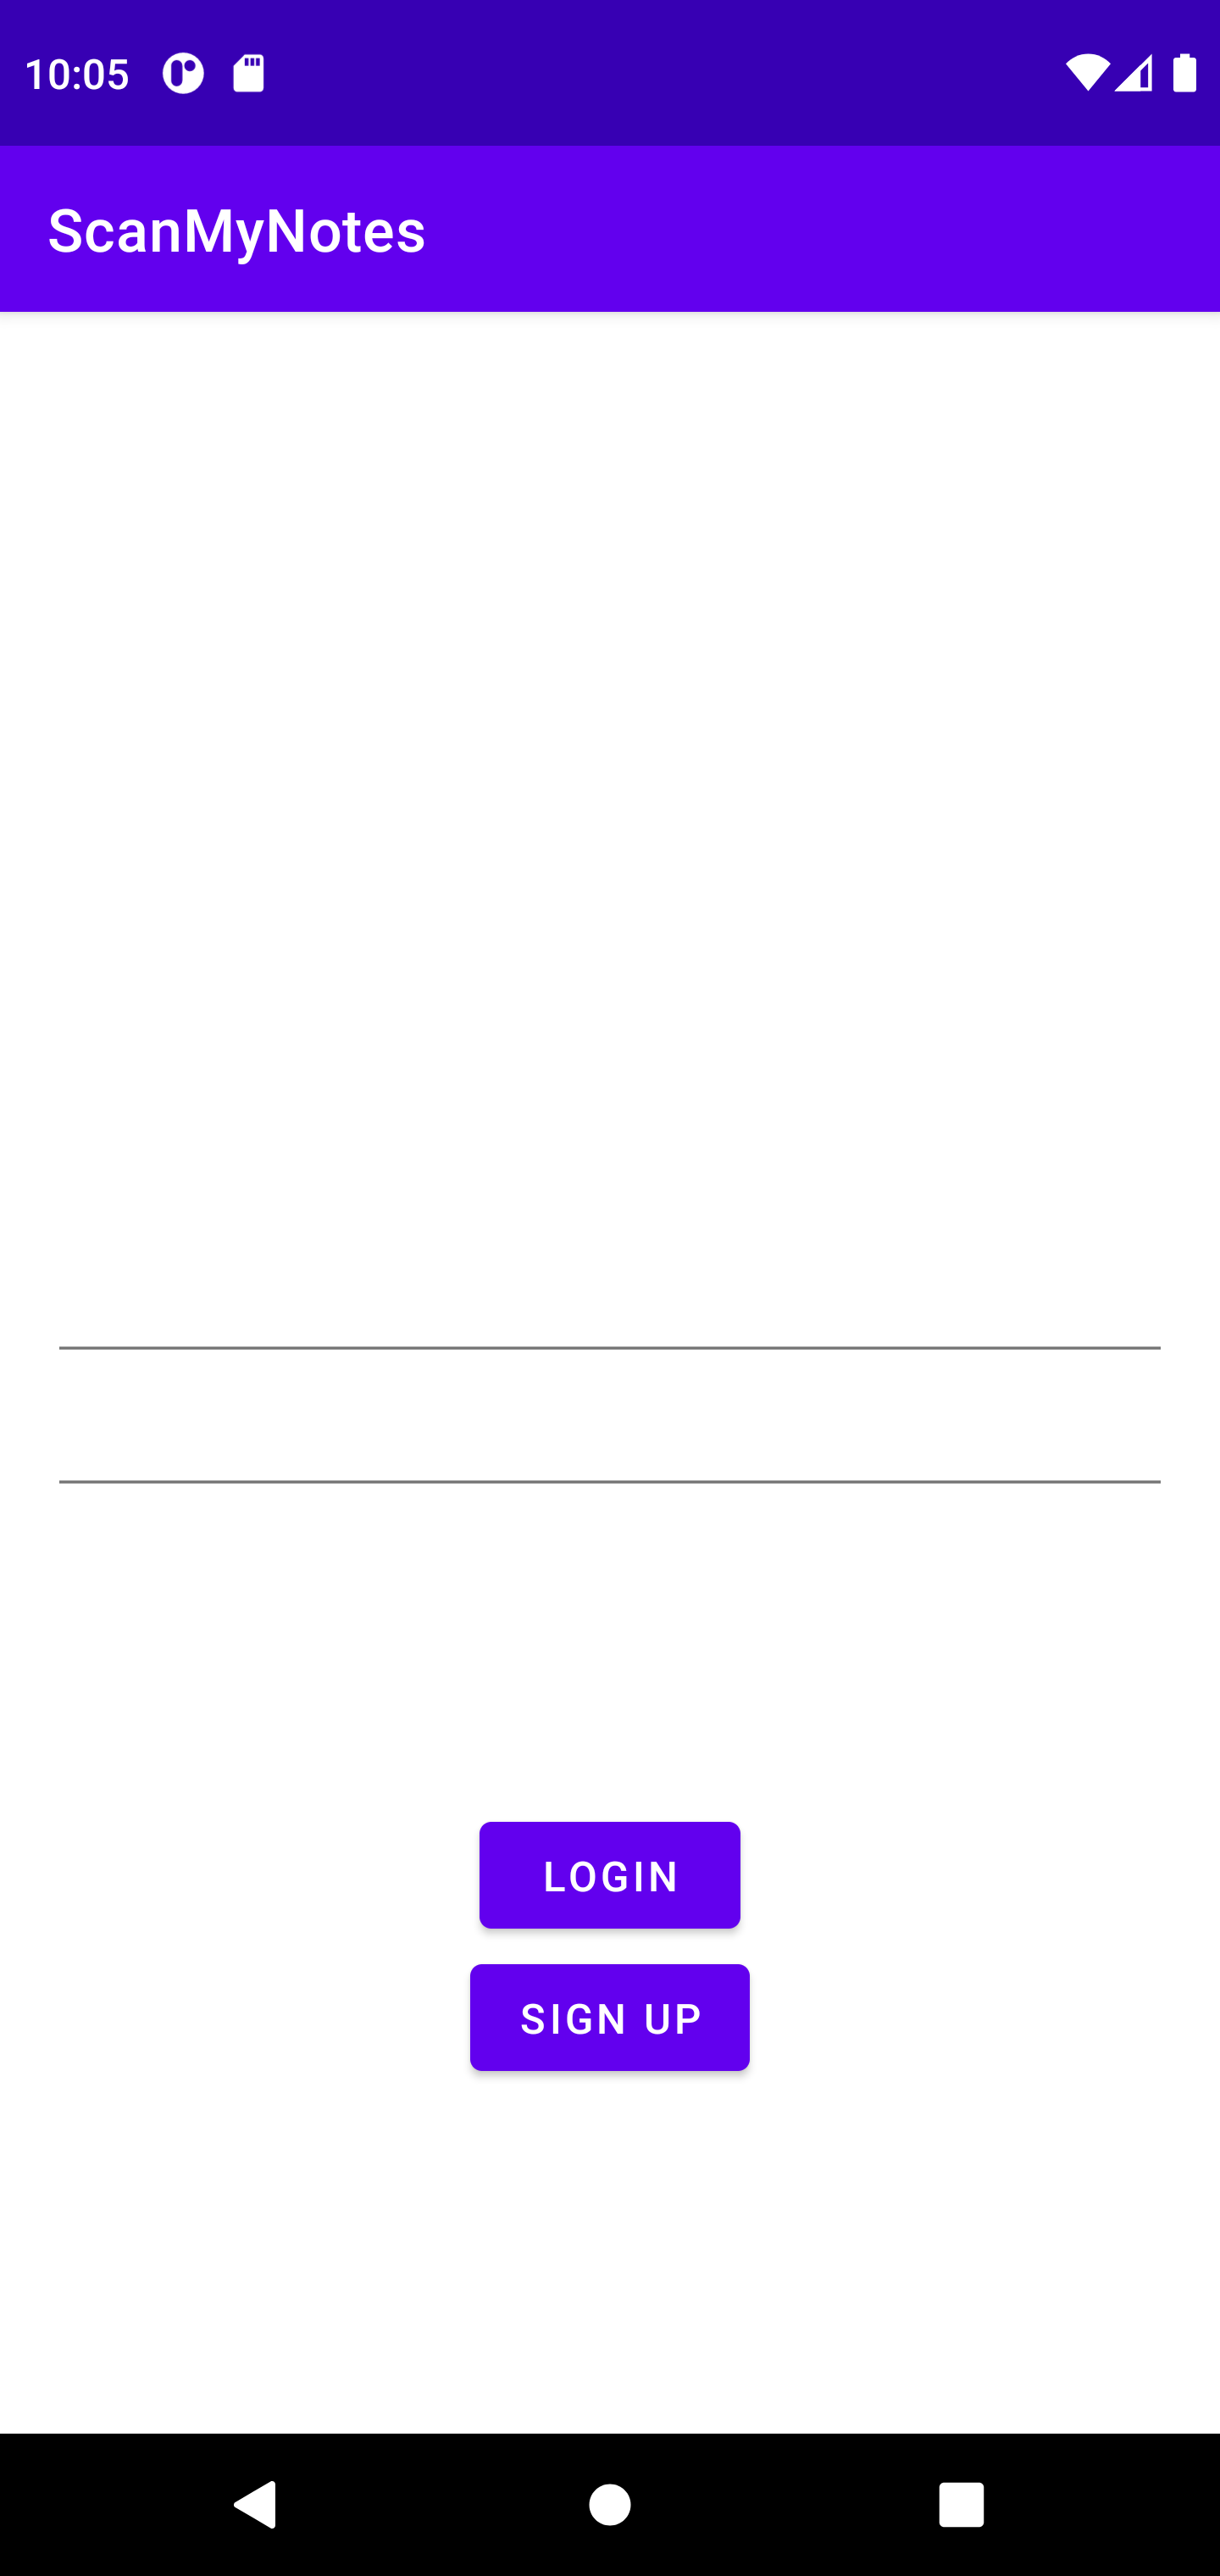
\includegraphics[width=60mm, keepaspectratio]{figures/login_screenshot_before.png}
	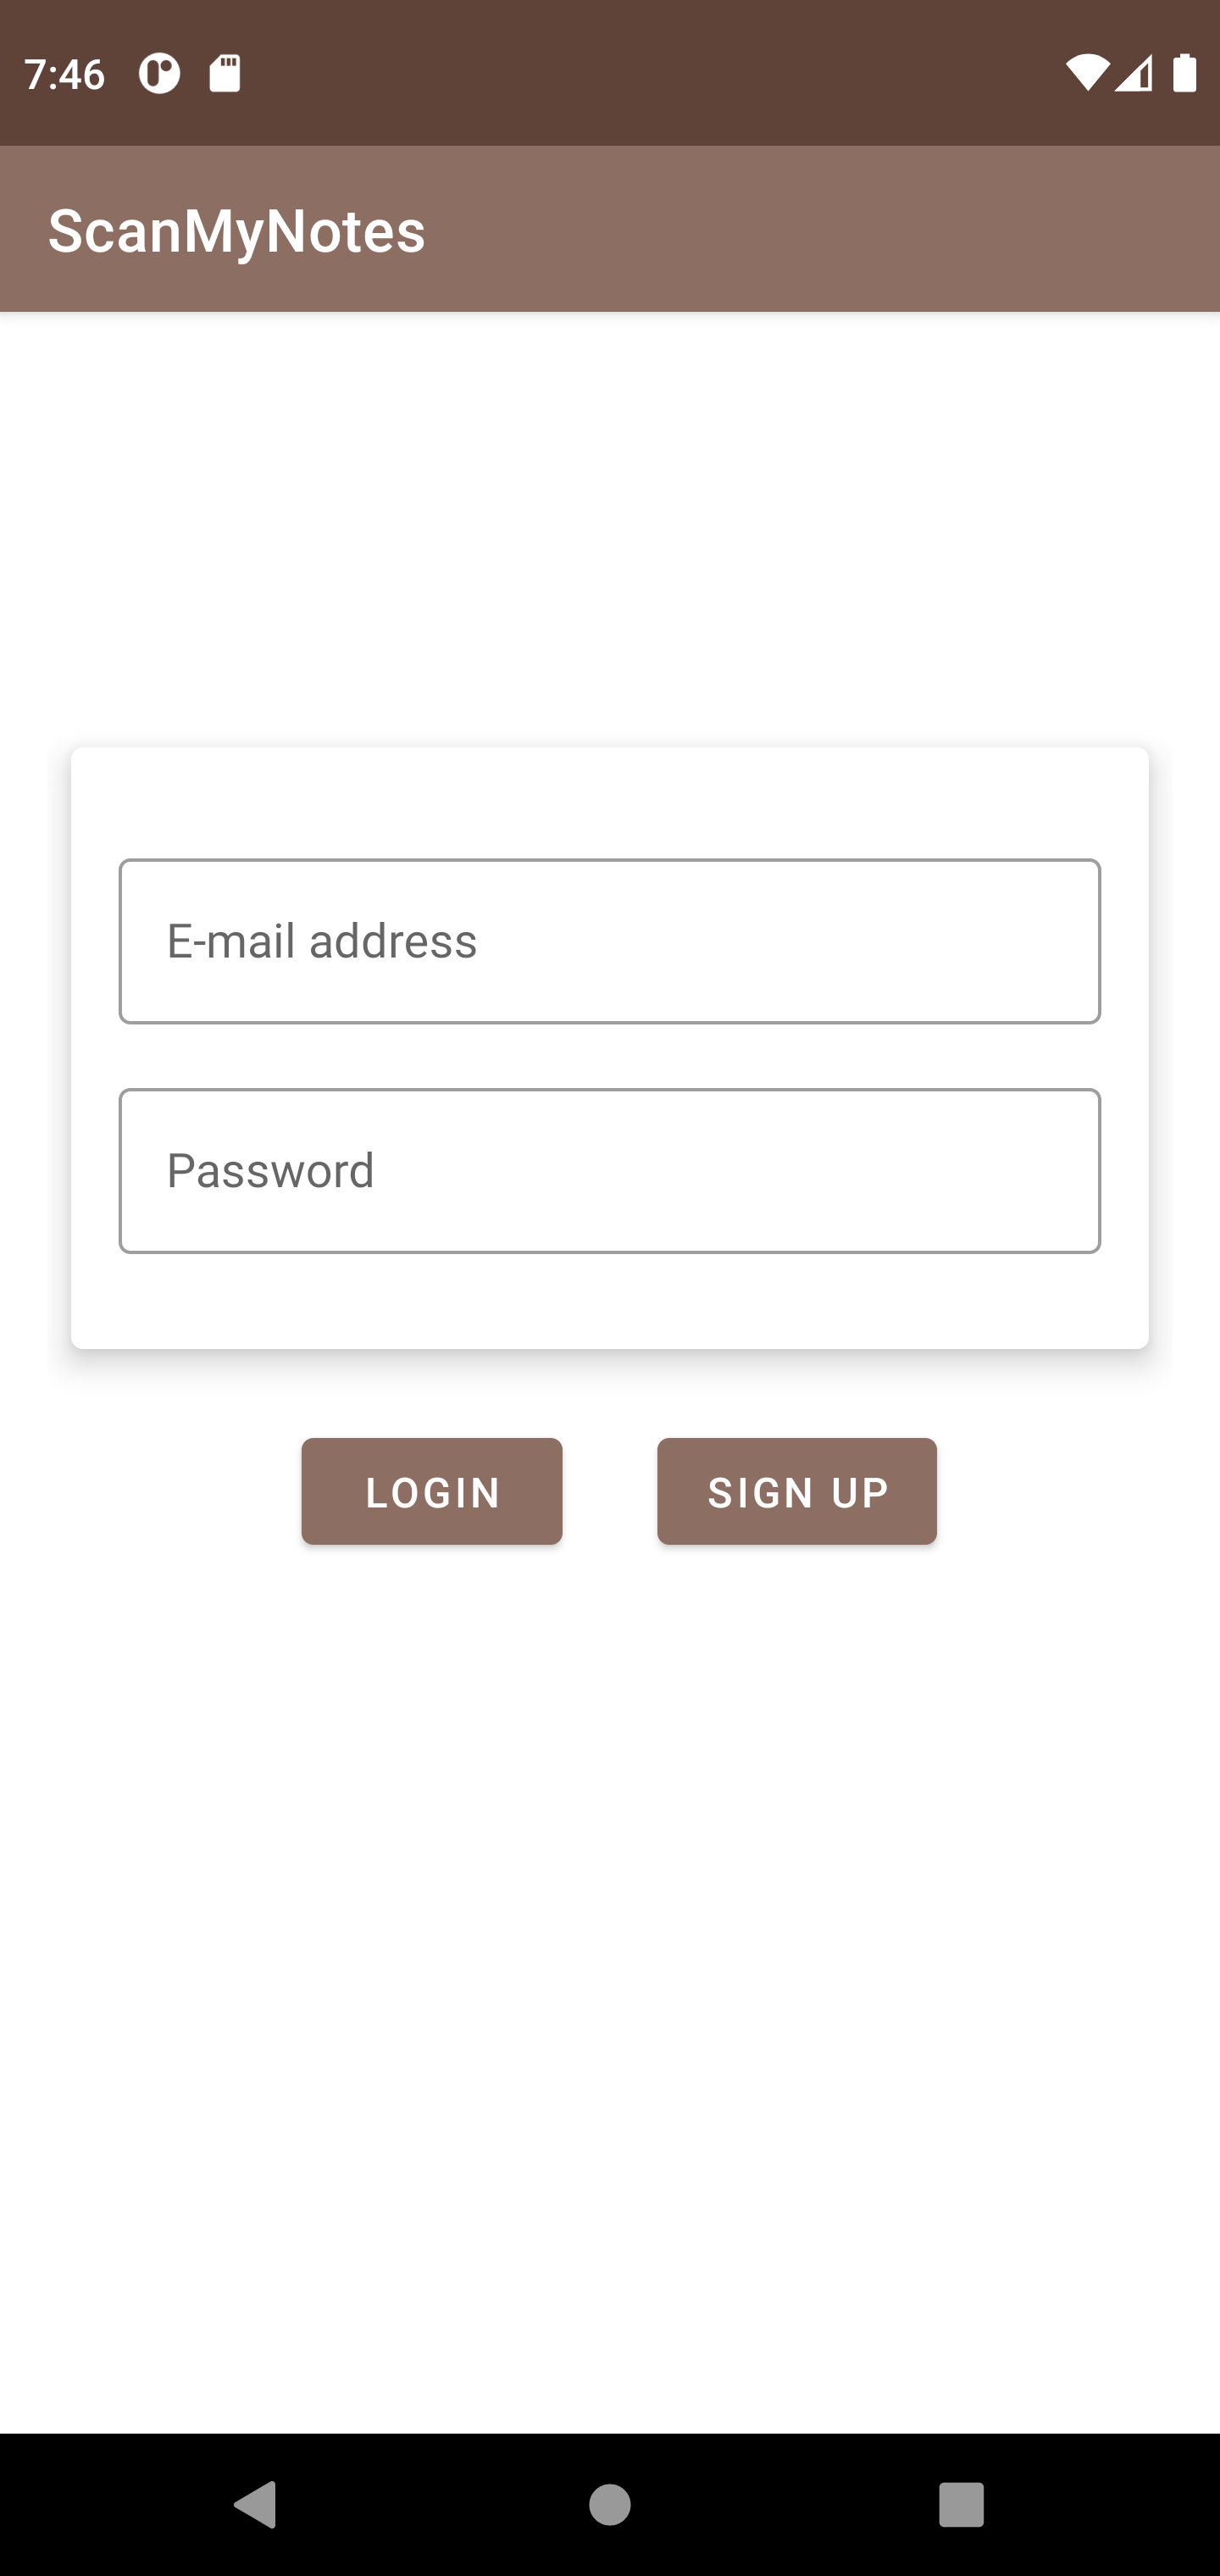
\includegraphics[width=60mm, keepaspectratio]{figures/login_screenshot_after.png}
	\caption{Bejelentkezési képernyő a Material komponensek és alapelvek alkalmazása előtt és után.}
	\label{fig:MaterialBeforeAfter}
\end{figure}

%TODO testing libs
\section{JUnit 4}

\section{Mockito}
\chapter{Követelmények}

A fejlesztés során alapvető célom volt egy, a modern paradigmáknak és a felhasználók elvárásainak megfelelő applikáció megalkotása. Törekedtem az objektumorientált szemlélet alkalmazására, a felelősségek szétválasztására és a maximális felhasználói élmény nyújtására. Fontos volt, hogy az alkalmazás folyamatai ne térjenek el nagymértékben attól, mint amit a felhasználók más applikációkban megszokhattak, és minden művelet meg legyen valósítva az adatokon, amire szükségük lehet.

Ezek alapján az alábbi követelmények fogalmazódtak meg az alkalmazással szemben:
\begin{enumerate}
	\item A felhasználónak legyen lehetősége fiókot létrehozni, e-mail cím és jelszó megadásával bejelentkezni, illetve fiókjából ki is lépni.
	\item Az adatok legyenek perzisztensen tárolva, az alkalmazás bezárásával, abból való kilépéssel vagy egy esetleges készülékcsere esetén se vesszenek el.
	\item Az adatok csak bejelentkezés után váljanak láthatóvá, minden felhasználó csak a saját adataihoz férhessen hozzá.
	\item A felhasználó képes legyen kategóriákat létrehozni a jegyzetek számára, ezeket akár tetszőleges mélységben további kategóriákba ágyazni.
	\item Legyen lehetőség jegyzetek létrehozására dokumentumok lefényképezése által. A szöveg digitalizálása után a jegyzet legyen címmel ellátható, kategóriába sorolható és a tartalma szerkeszthető.
	\item Inkonzisztens adatok létrehozására ne adjon lehetőséget, a felhasználói input mindig legyen validálva.
	\item A jegyzeteken és kategóriákon lehessen minden fő műveletet - létrehozás, olvasás, módosítás, törlés - elvégezni, ezek során a felhasználói felület és az adatbázis maradjanak konzisztensek egymással.
	\item Módosítás során lehessen a jegyzetet újabb fényképek készítésével kiegészíteni, az ily módon digitalizált szöveg kerüljön hozzáfűzésre az eredeti tartalomhoz.
	\item A UI esztétikai és felhasználói élmény szempontjából legyen megfelelő, a hosszú ideig tartó folyamatokat jelezze a felhasználónak töltőképernyő segítségével.
	\item A jegyzetek listája lehessen rendezhető és kereshető.
\end{enumerate}
\chapter{Alkalmazás működése}

A következőkben az alkalmazás funkcióit fogom bemutatni, a leírásokat képernyőképekkel kiegészítve. A képek néhol eltérnek egymástól, melynek oka hogy az applikáció funkcionalitásából fakadóan nem volt lehetséges mindet az emulátoron elkészíteni, hanem a jegyzetek készítéséhez fizikai készülékre is szükség volt.

\section{Bejelentkezés}
A telepítést követően a bejelentkezési képernyő az első, amivel a felhasználó találkozik. Ez már korábban megjelent a dolgozatban, a \refstruc{fig:MaterialBeforeAfter} bemutatásában. Itt a beviteli mezők segédszövegei egyértelműsítik, hogy milyen adatok elvártak a bejelentkezéshez illetve regisztrációhoz. Ezek gombnyomás hatására validálásra kerülnek, és amennyiben az e-mail formátuma nem érvényes vagy a jelszó hossza nem éri el a 6 karaktert, akkor a folyamat meghiúsul, és a felhasználó értesül róla, hogy mely mező(k) tartalmát kell javítania.

\section{Kategorizált lista}
Sikeres bejelentkezést követően az alkalmazás a fő képernyőjére navigál, ahol az eddig elmentett jegyzeteket láthatjuk kategóriákba rendezve. A kategóriák alapértelmezetten össze vannak csukva, csak a legfelső szinten található elemeket látjuk. A lista sorainak jobb szélén elhelyezkedő nyilakra kattintva tudjuk kibontani az adott kategóriát, ezzel megtekinteni a tartalmát (\refstruc{fig:NoteListScreen}).

\begin{figure}[!ht]
	\centering
	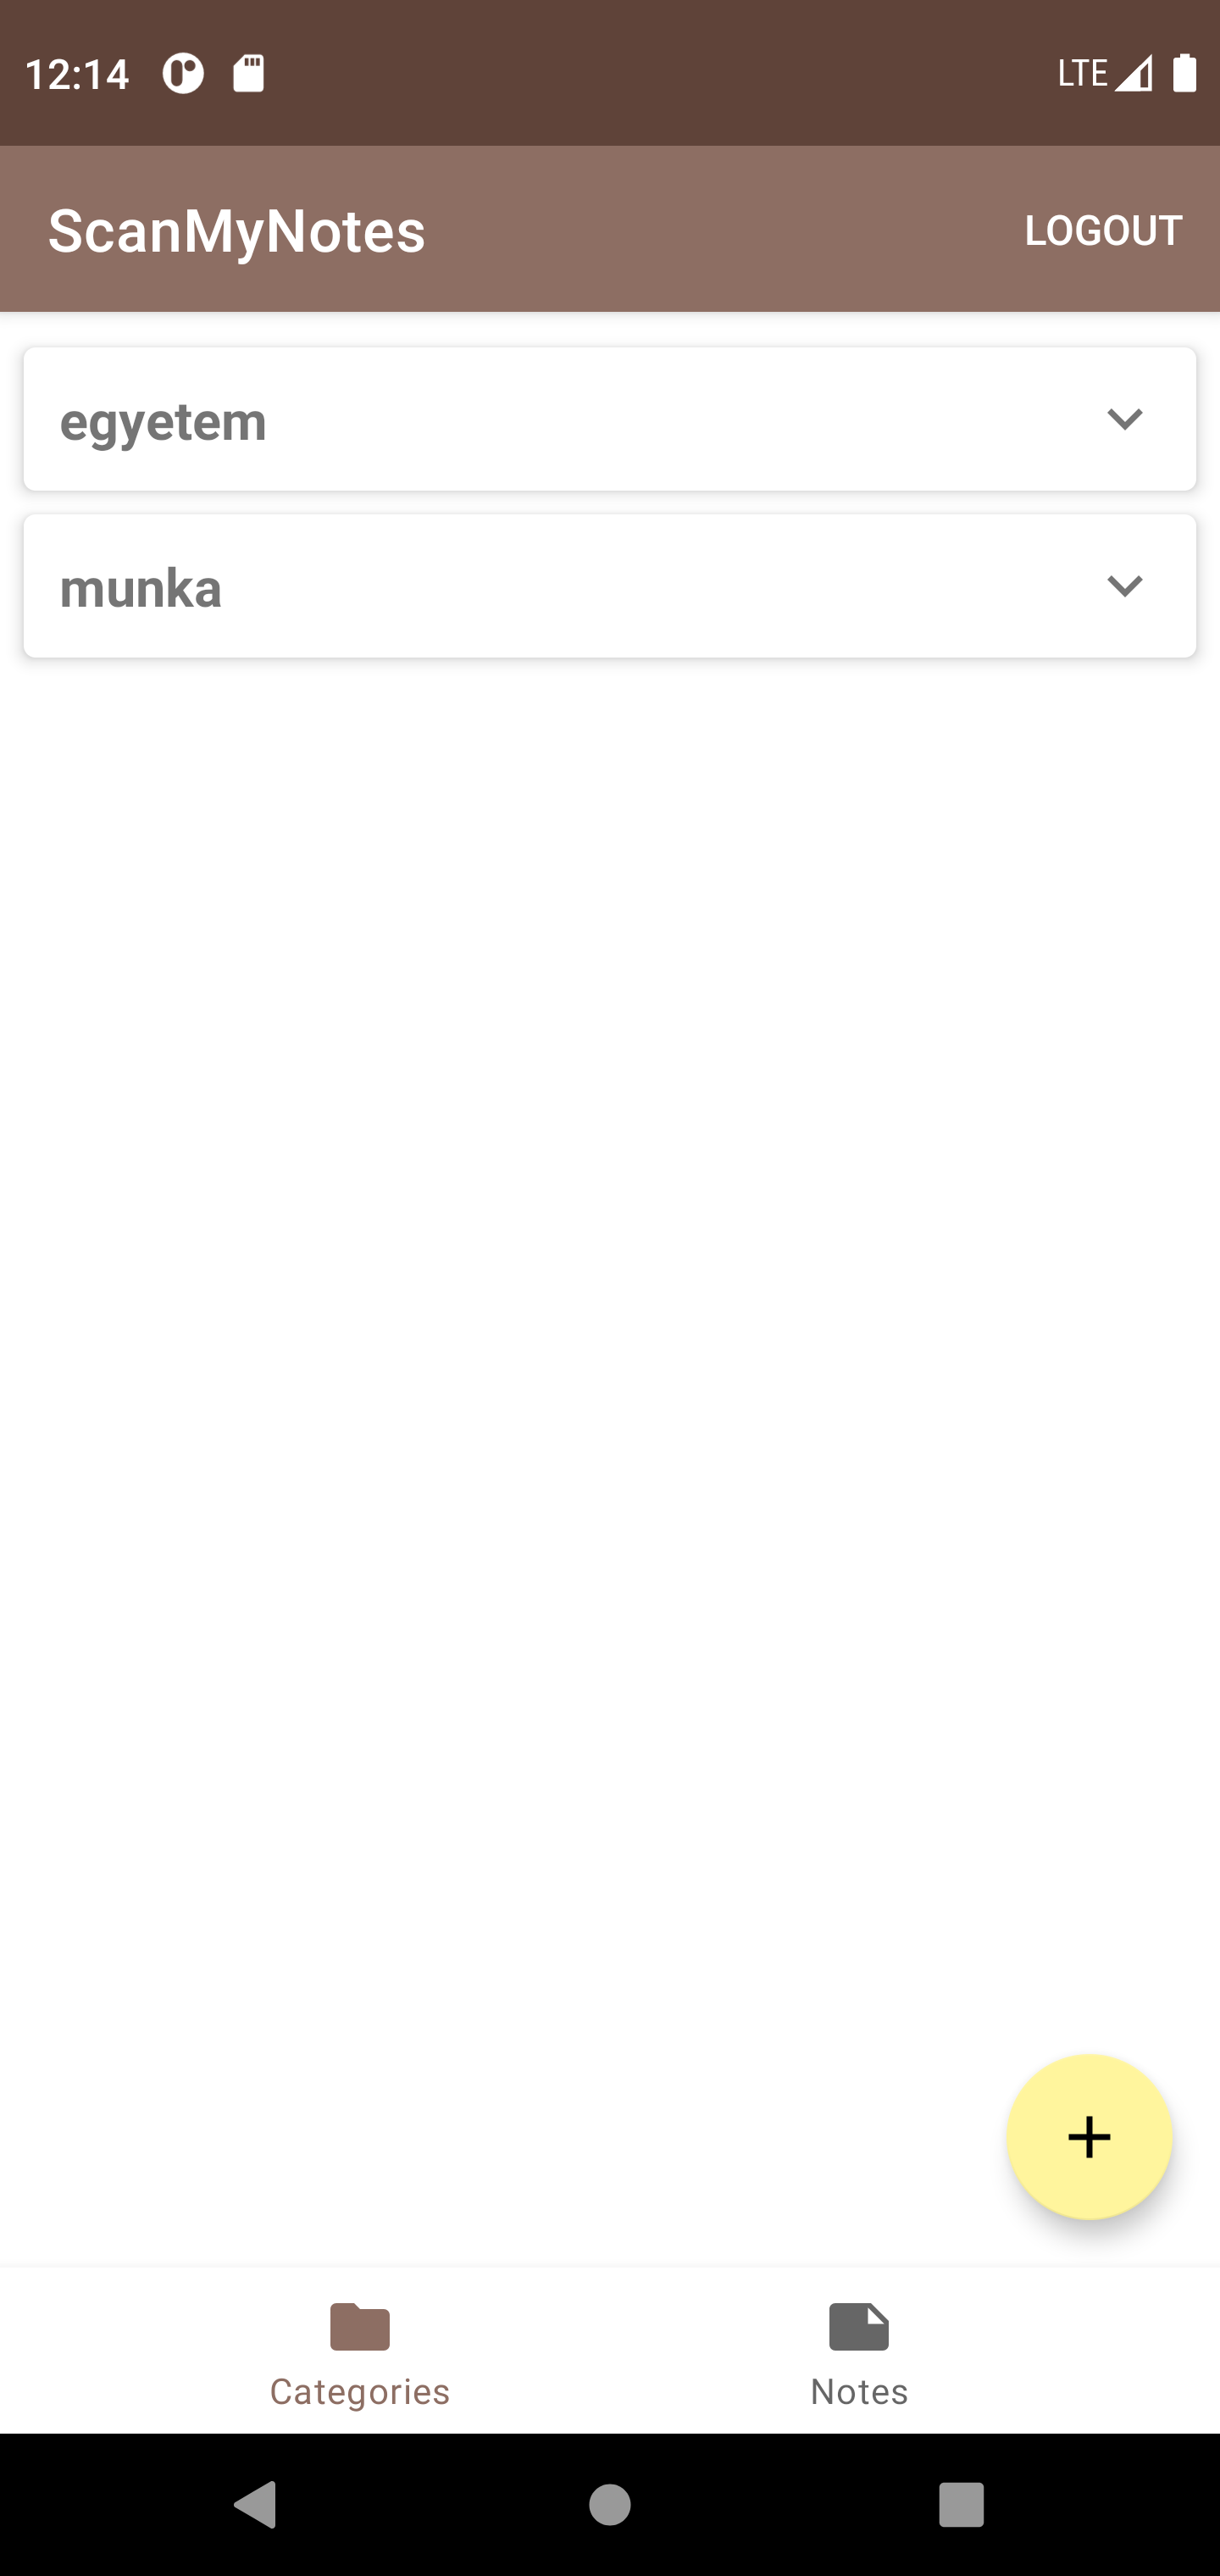
\includegraphics[width=55mm, keepaspectratio]{figures/notelist_closed.png}
	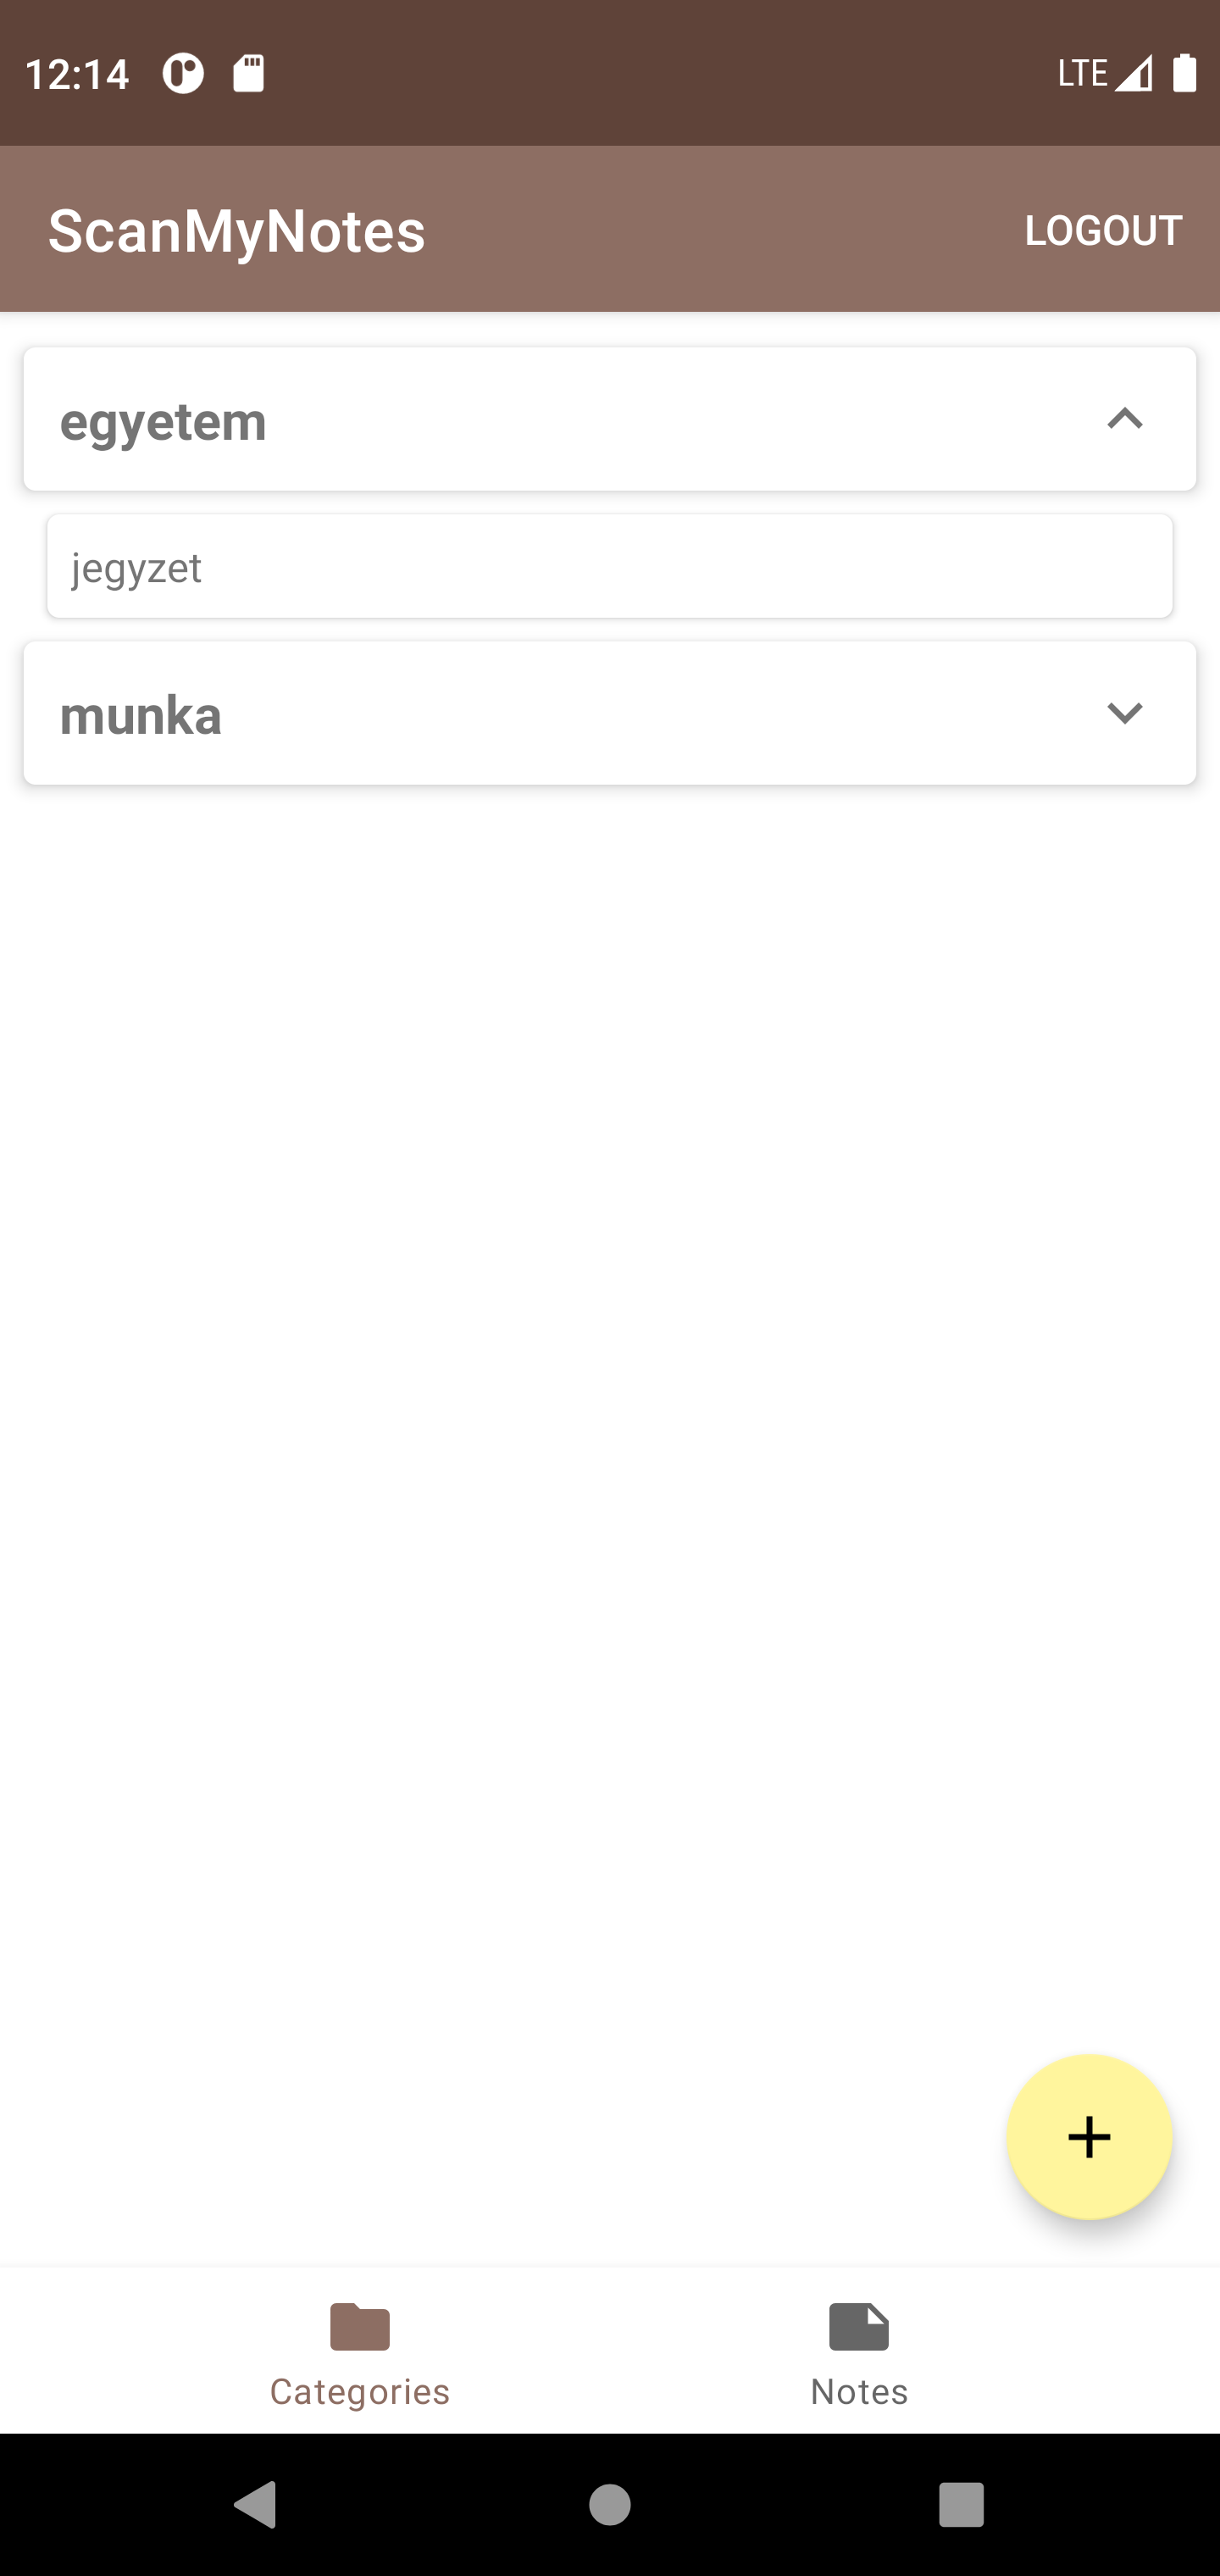
\includegraphics[width=55mm, keepaspectratio]{figures/notelist_open.png}
	\caption{Az alkalmazás kezdőlapja alapértelmezett állapotban, illetve egy kategória kibontva.}
	\label{fig:NoteListScreen}
\end{figure}

Innen számos lehetőségünk adódik navigációra az applikáción belül, kezdve a jobb felső sarokban található, meglehetősen magától értetődő kijelentkezés gombbal. Ezt megnyomva a fent leírt bejelentkezési képernyőre navigálunk, ahol adataink megadásával újra bejelentkezhetünk.
\newpage
\section{Jegyzetlista}
A főképernyőn alul egy navigációs sávot találunk, mellyel a két különböző listamegjelenítés között tudunk váltani. Míg a \emph{Categories} opció alatt egy hierarchikusan egymás alá rendezett listát láthatunk, a \emph{Notes} opció csak a jegyzeteket tárja elénk, kategóriától függetlenül. Itt több lehetőség tárul elénk: a képernyő tetején található egy keresősáv és egy rendezés gomb. Keresni a jegyzetek címe alapján tudunk, itt gépelés közben azonnal szűkül az eredményhalmaz. A rendezés szintén a cím alapján működik, jelenleg növekvő és csökkenő betűrendet támogat az alkalmazás (\refstruc{fig:NoteListScreen2}).

\begin{figure}[!ht]
	\centering
	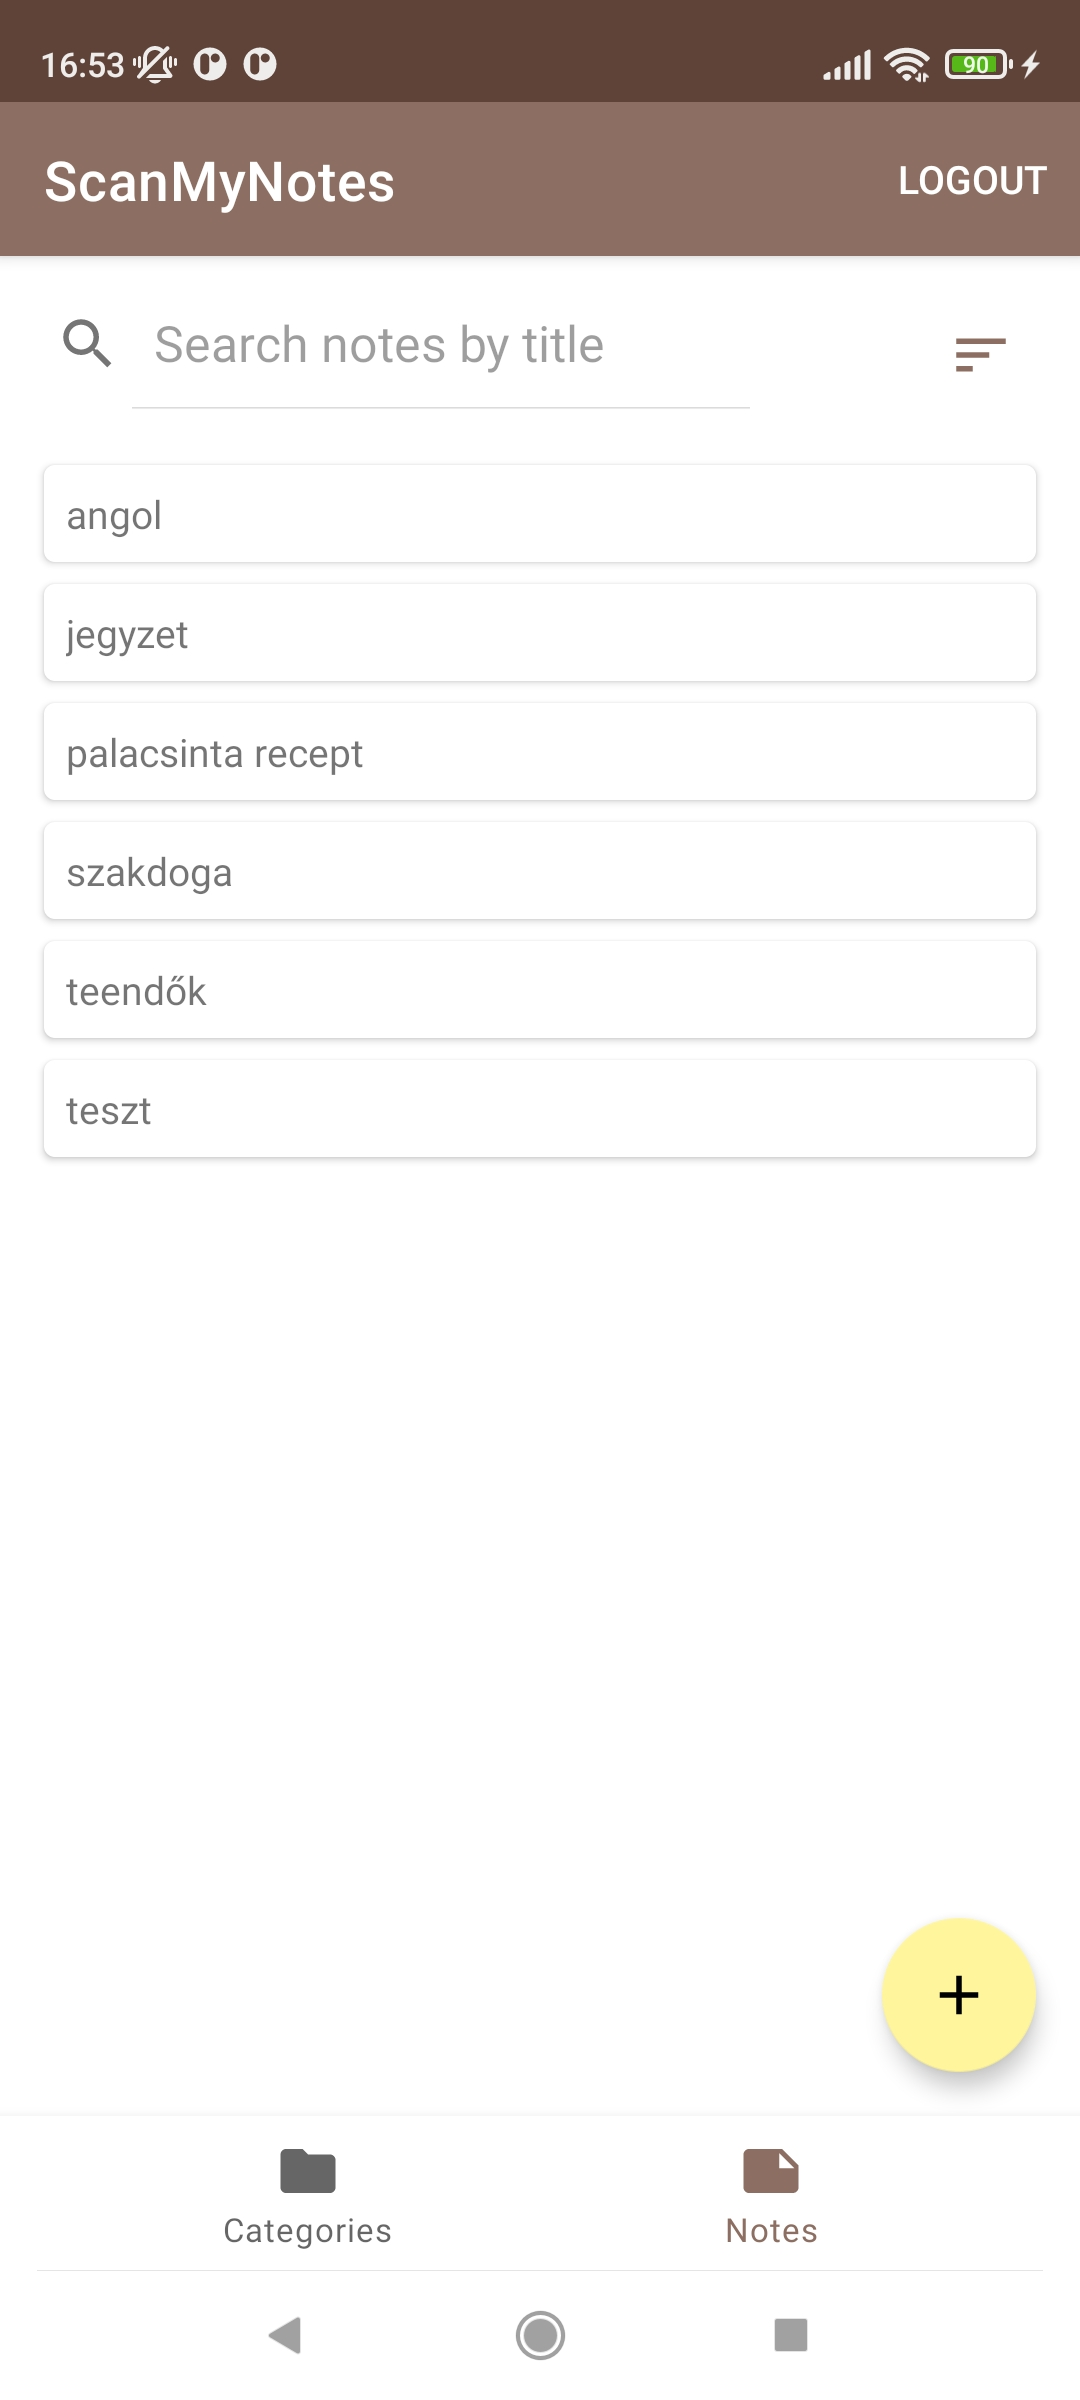
\includegraphics[width=49mm, keepaspectratio]{figures/notelist_full.jpg}
	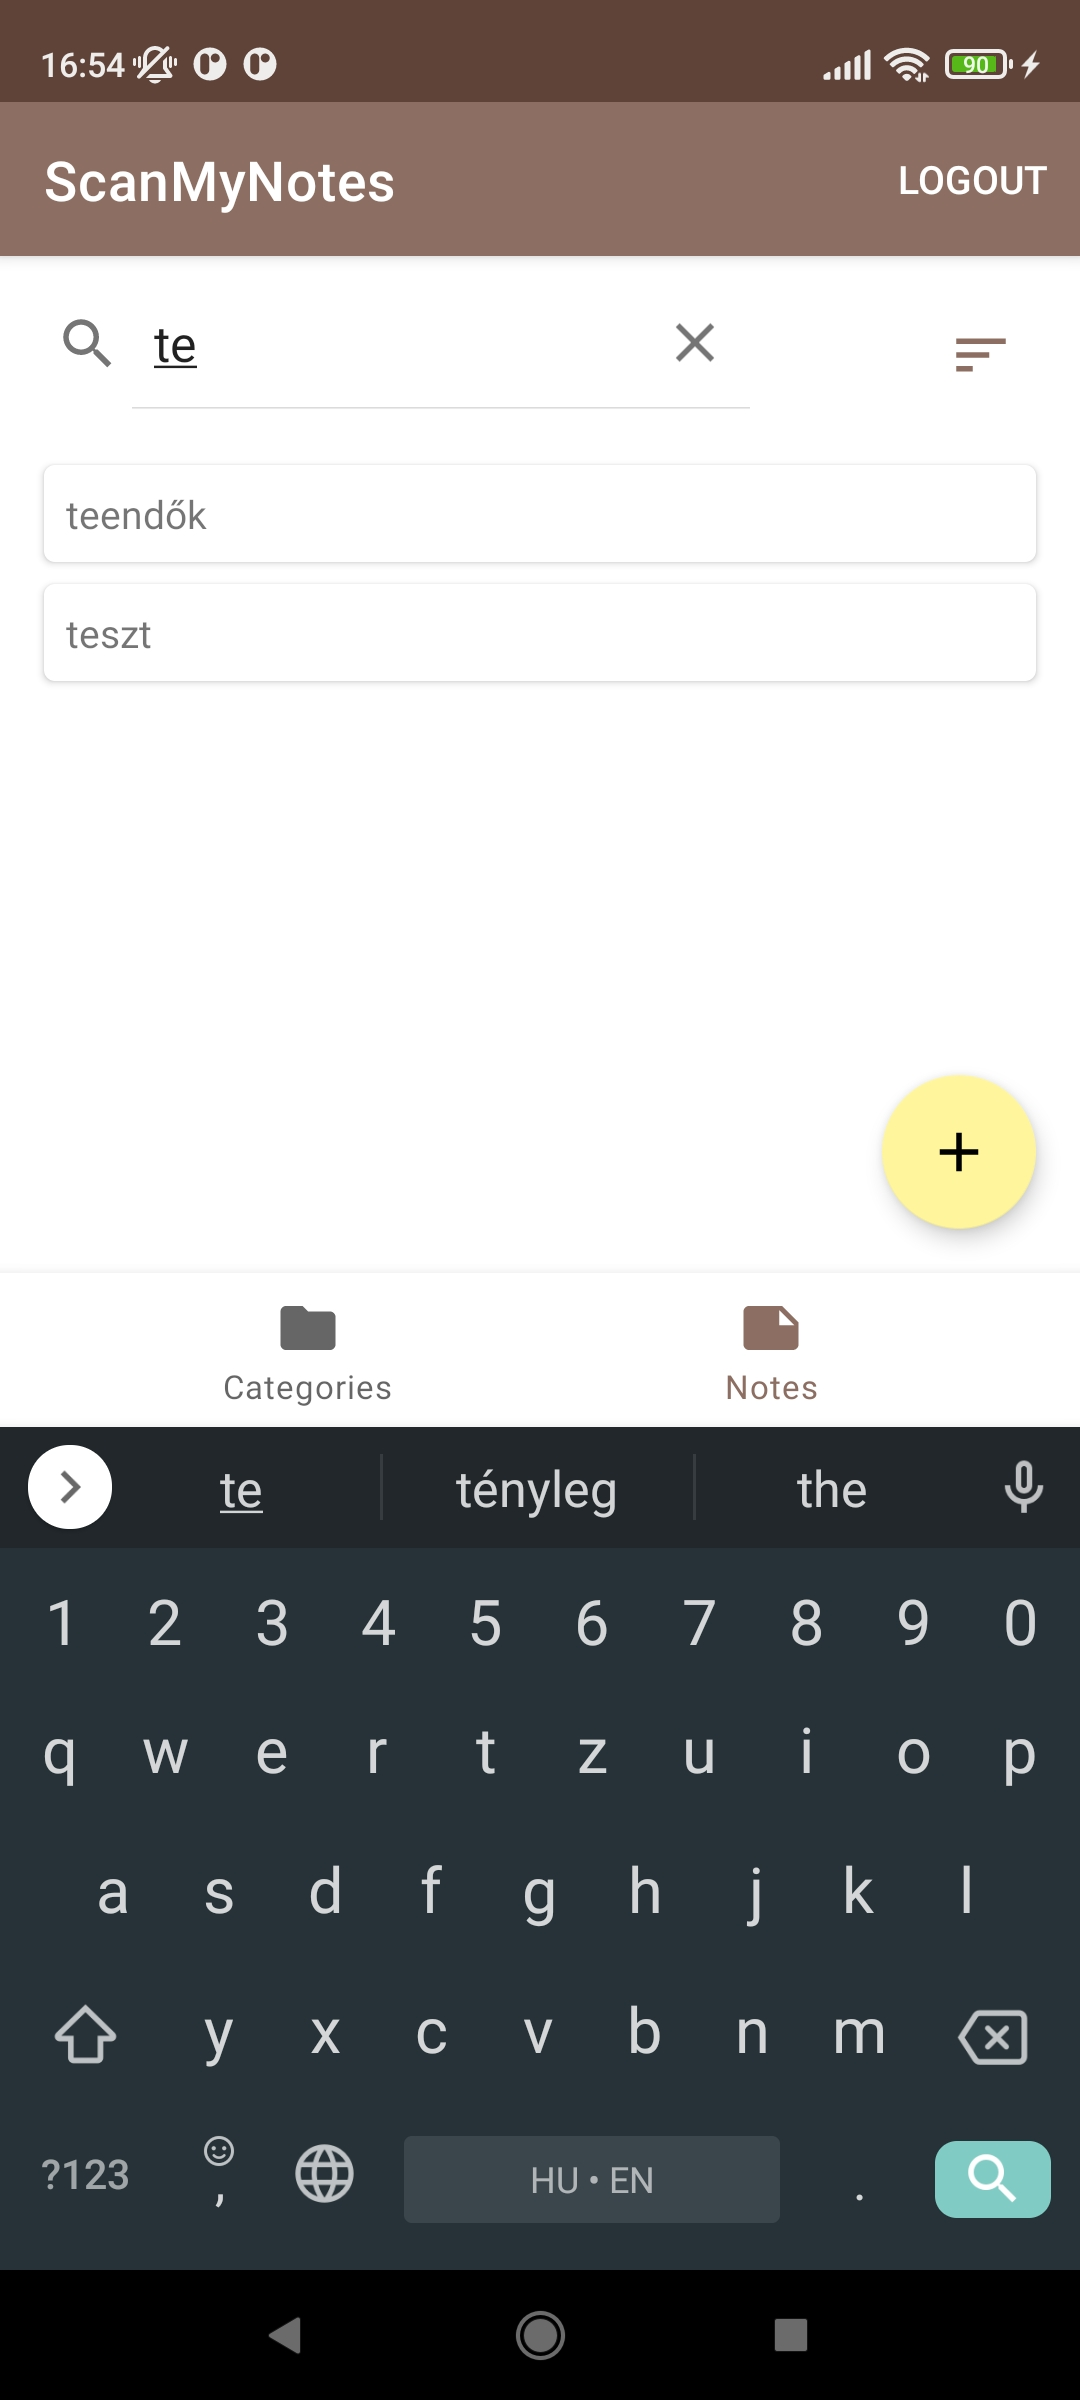
\includegraphics[width=49mm, keepaspectratio]{figures/notelist_search.jpg}
	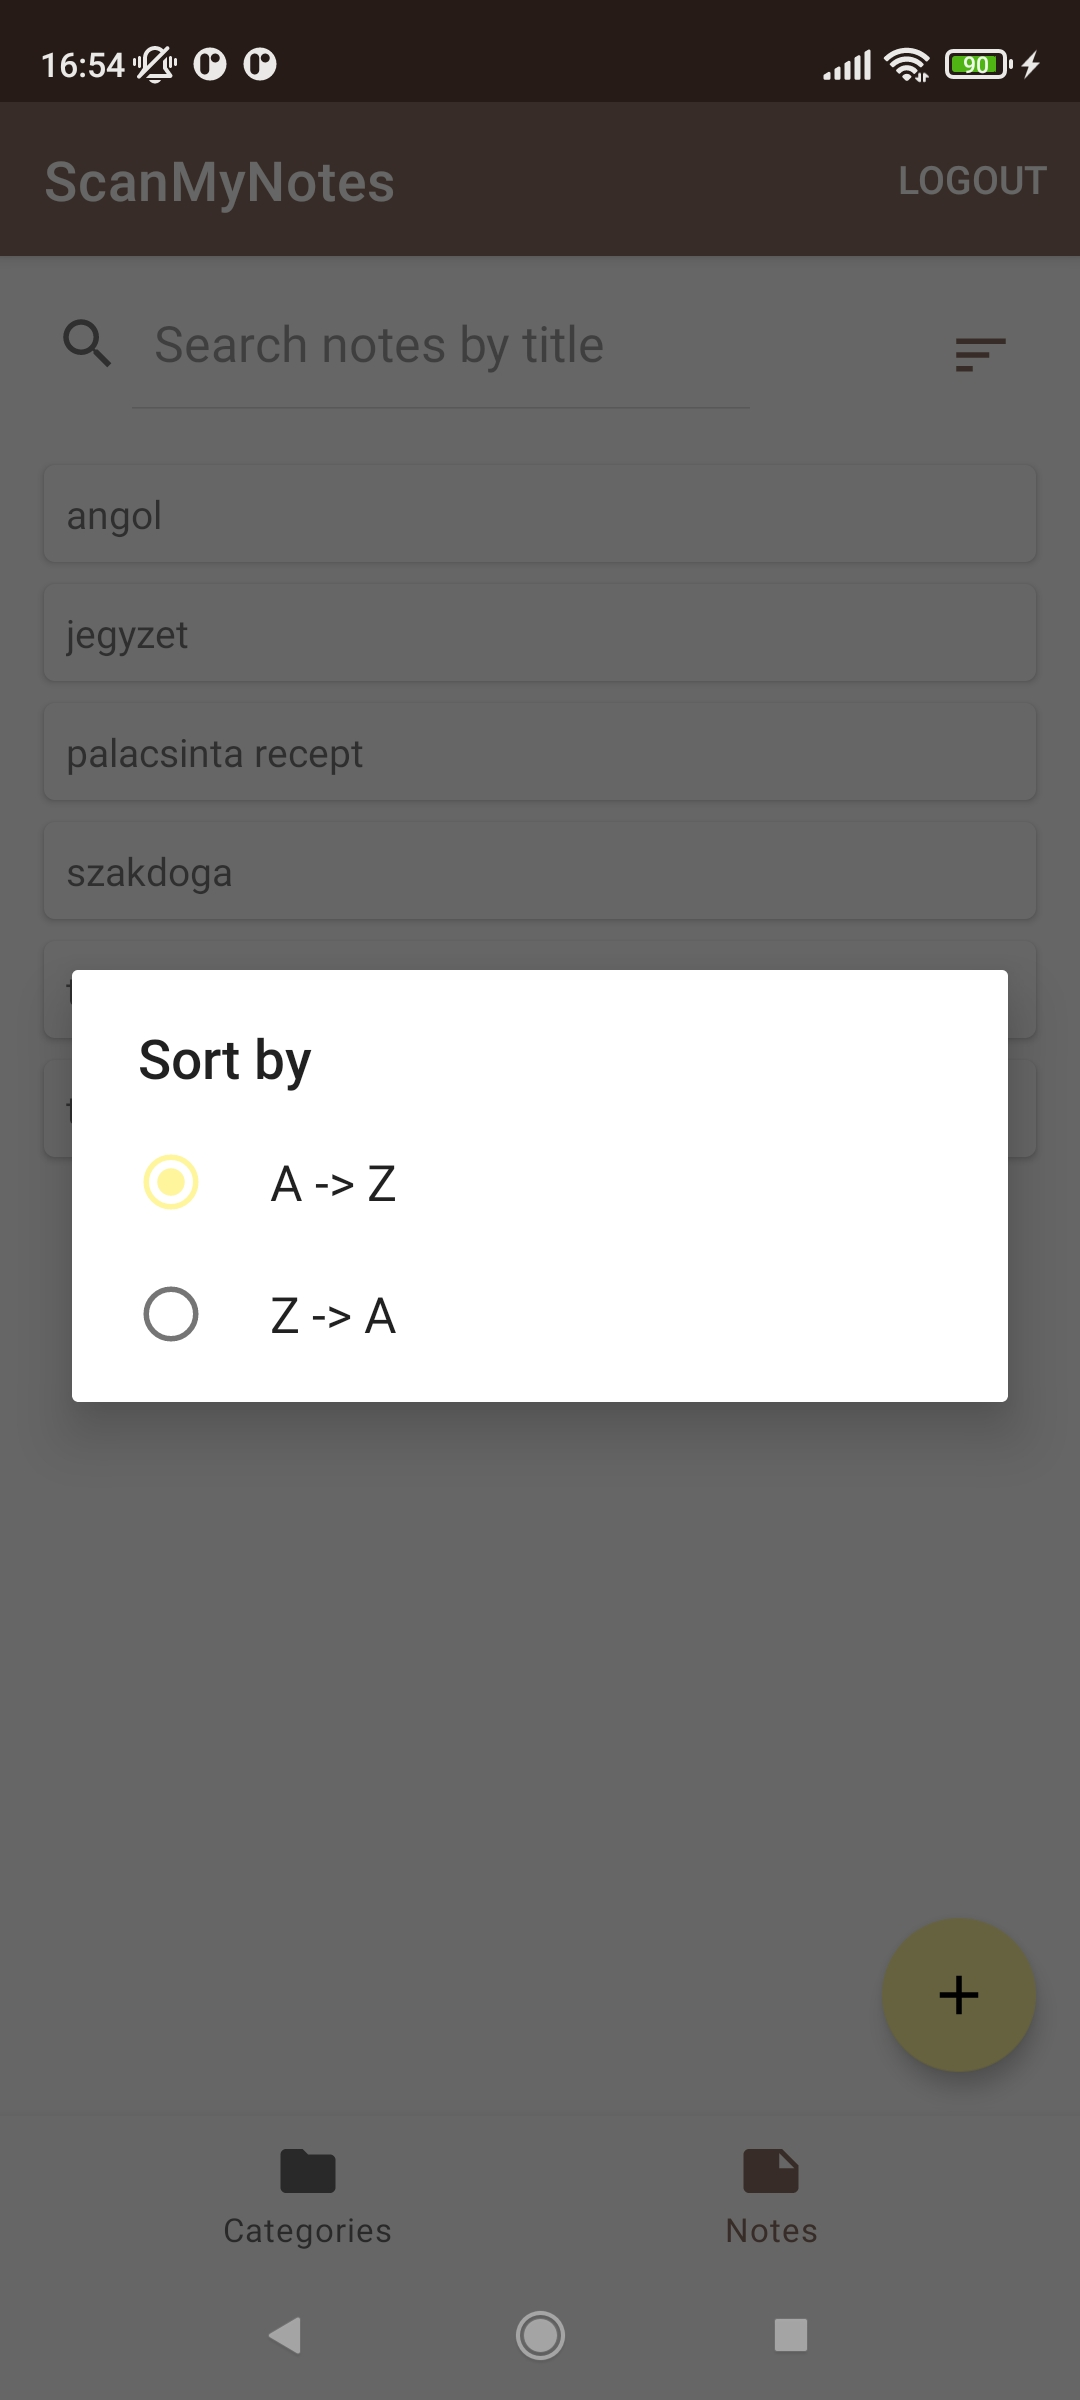
\includegraphics[width=49mm, keepaspectratio]{figures/notelist_sort.jpg}
	\caption{A jegyzetek listája, és a rajta elvégezhető műveletek.}
	\label{fig:NoteListScreen2}
\end{figure}
\newpage
\section{Jegyzet létrehozása}
Az alkalmazás fő funkcionalitása a jegyzetek tárolása, így elég fontos, hogy legyen lehetőség újak létrehozására. Ez a képernyő jobb alsó sarkában található plusz gombra kattintva tehető meg. Az ott megjelenő két újabb gomb közül az alsó megnyomására felugrik egy kameraablak, ahol egy fénykép készítése után megtörténik a digitalizáció, és a szerkesztési oldalra ugrunk. Itt egy cím megadásával fejezhetjük be a létrehozási folyamatot, de opcionálisan hozzárendelhetjük egy kategóriához is (\refstruc{fig:NewNoteScreen}). Amíg a cím vagy a tartalom üres, addig az alkalmazás nem fogja engedni elmenteni a jegyzetet, figyelmeztetést rak az üresen hagyott mezőre.
\begin{figure}[!ht]
	\centering
	
\includegraphics[width=55mm, keepaspectratio]{figures/newnote_photo.jpg}
	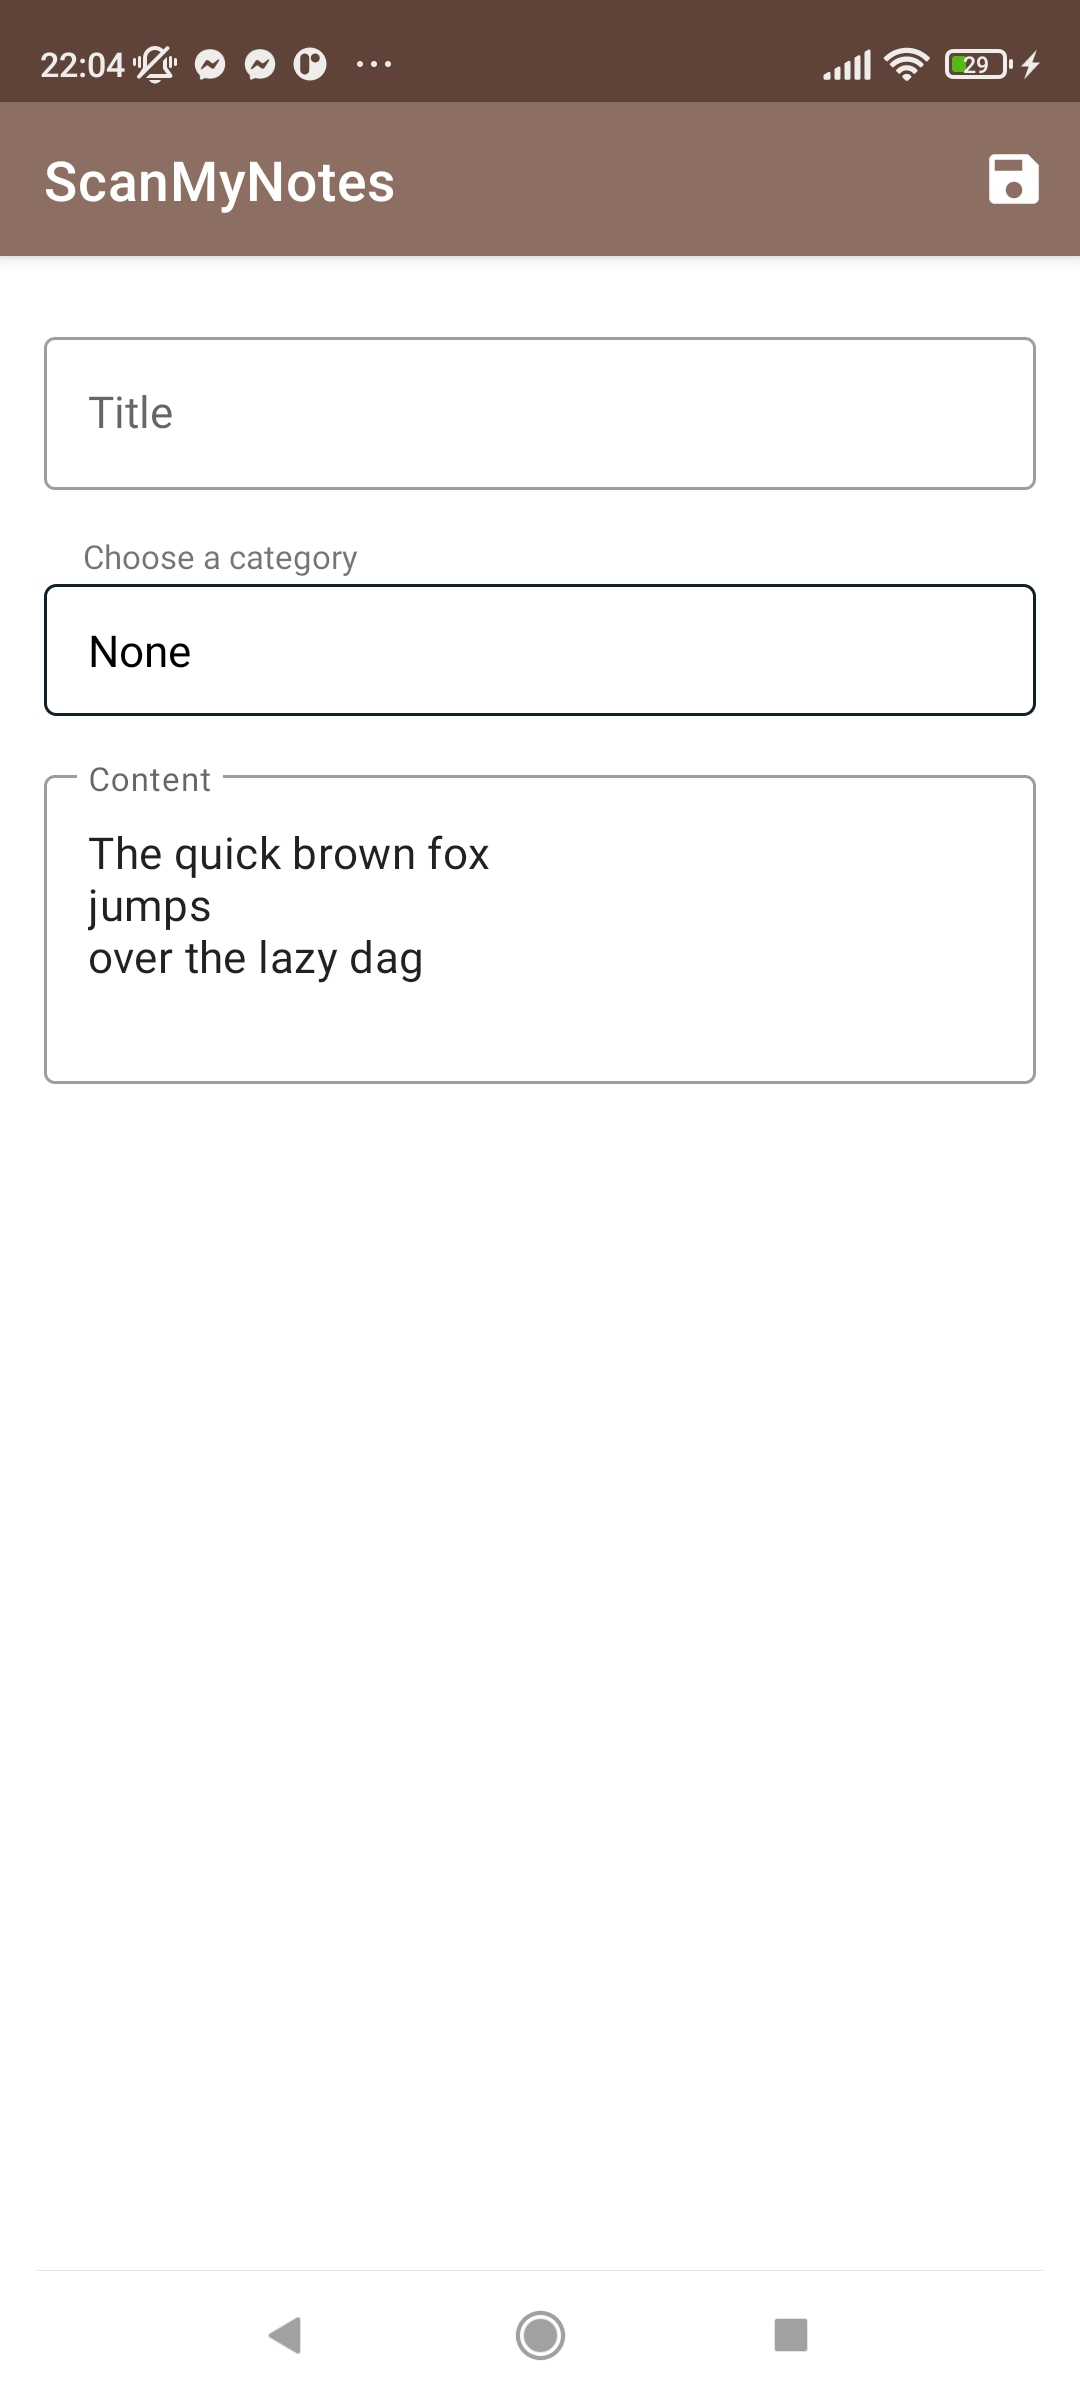
\includegraphics[width=55mm, keepaspectratio]{figures/newnote_create.jpg}
	\caption{A létrehozás során készített kép, illetve az abból kialakuló jegyzet szerkesztése.}
	\label{fig:NewNoteScreen}
\end{figure}
\newpage
\section{Jegyzet szerkesztése}
Amennyiben a listában egy jegyzetre kattintunk, illetve újat hozunk létre, akkor annak részletes oldalára navigálunk. Itt megtekinthetjük a tartalmát, a jobb felső sarokban található ceruza ikonra nyomva pedig szerkeszthetjük is (\refstruc{fig:NoteDetailsScreen}). Megváltoztathatjuk a címét, tartalmát, kategóriáját, a fent megjelenő pluszjel segítségével pedig készíthetünk újabb fotót, melynek szövege hozzáfűzésre kerül az eddigihez. A fentebb említett megkötések itt is érvényesek, azaz a cím és a tartalom nem lehet üres az elmentés pillanatában.

Mind megtekintési, mind szerkesztési módban elérhető a fenti sávban a szemetes ikon, mellyel törölhetjük a jegyzetet a listánkból. Vigyázat, ez a művelet nem visszafordítható!

\begin{figure}[!ht]
	\centering
	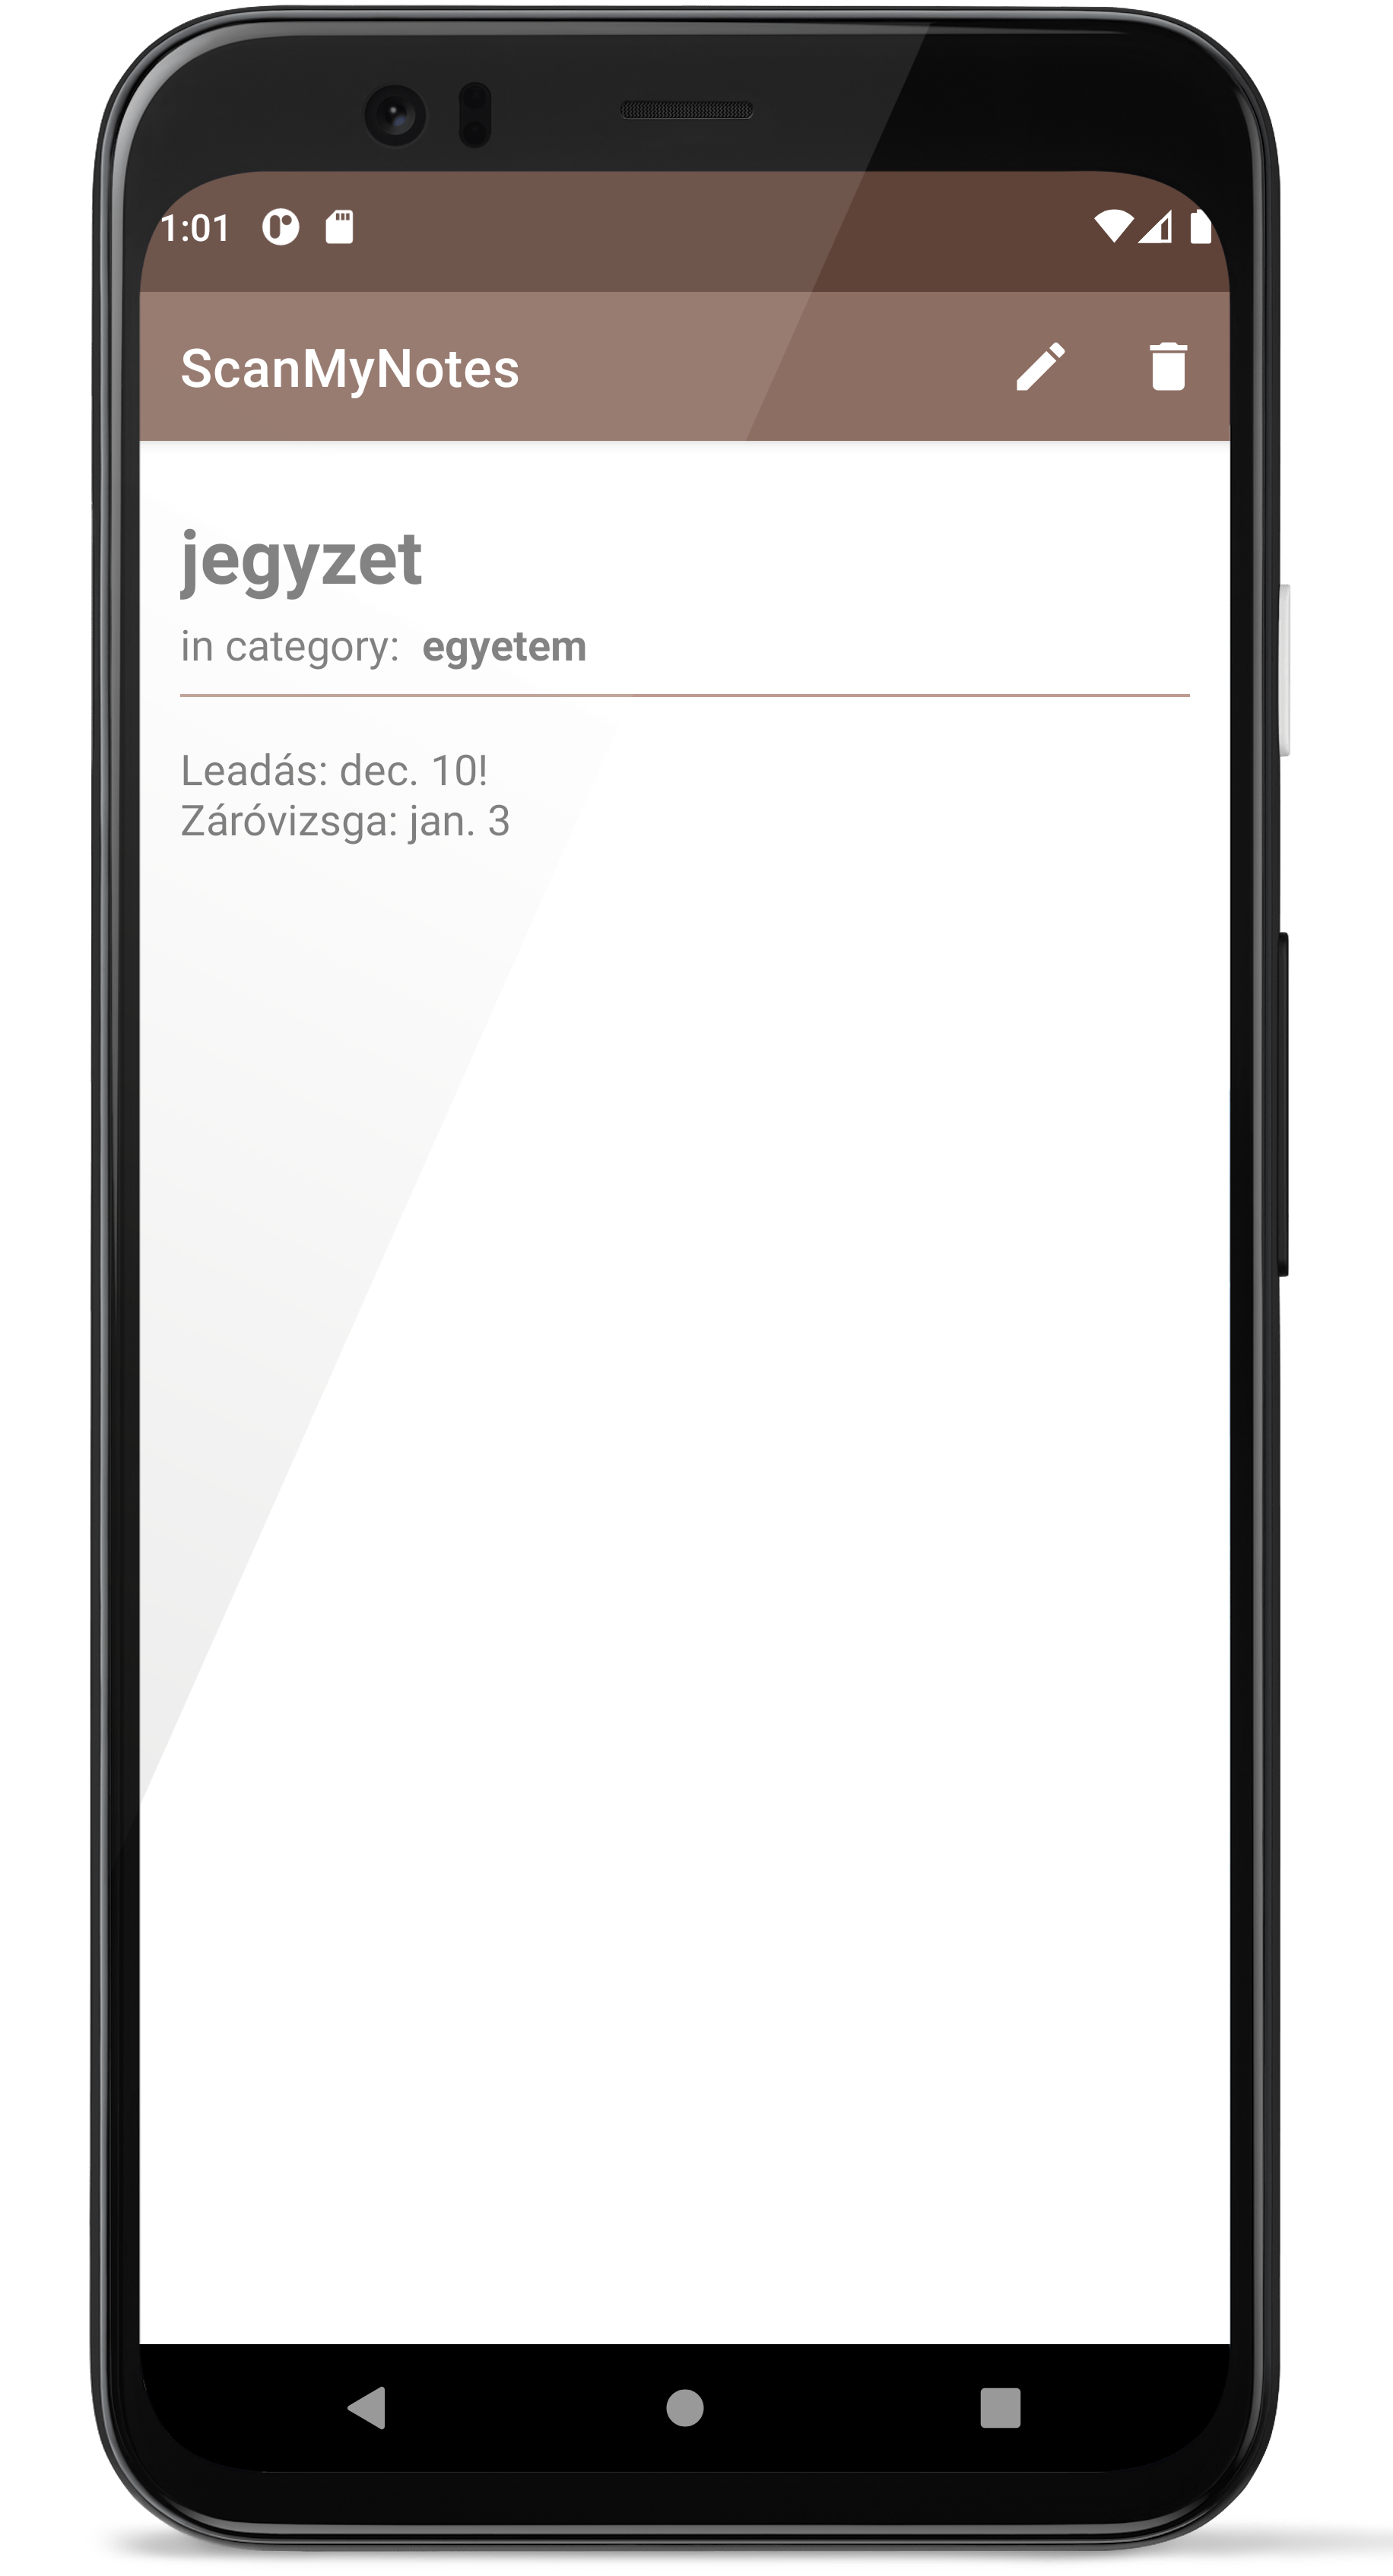
\includegraphics[width=55mm, keepaspectratio]{figures/note_view.png}
	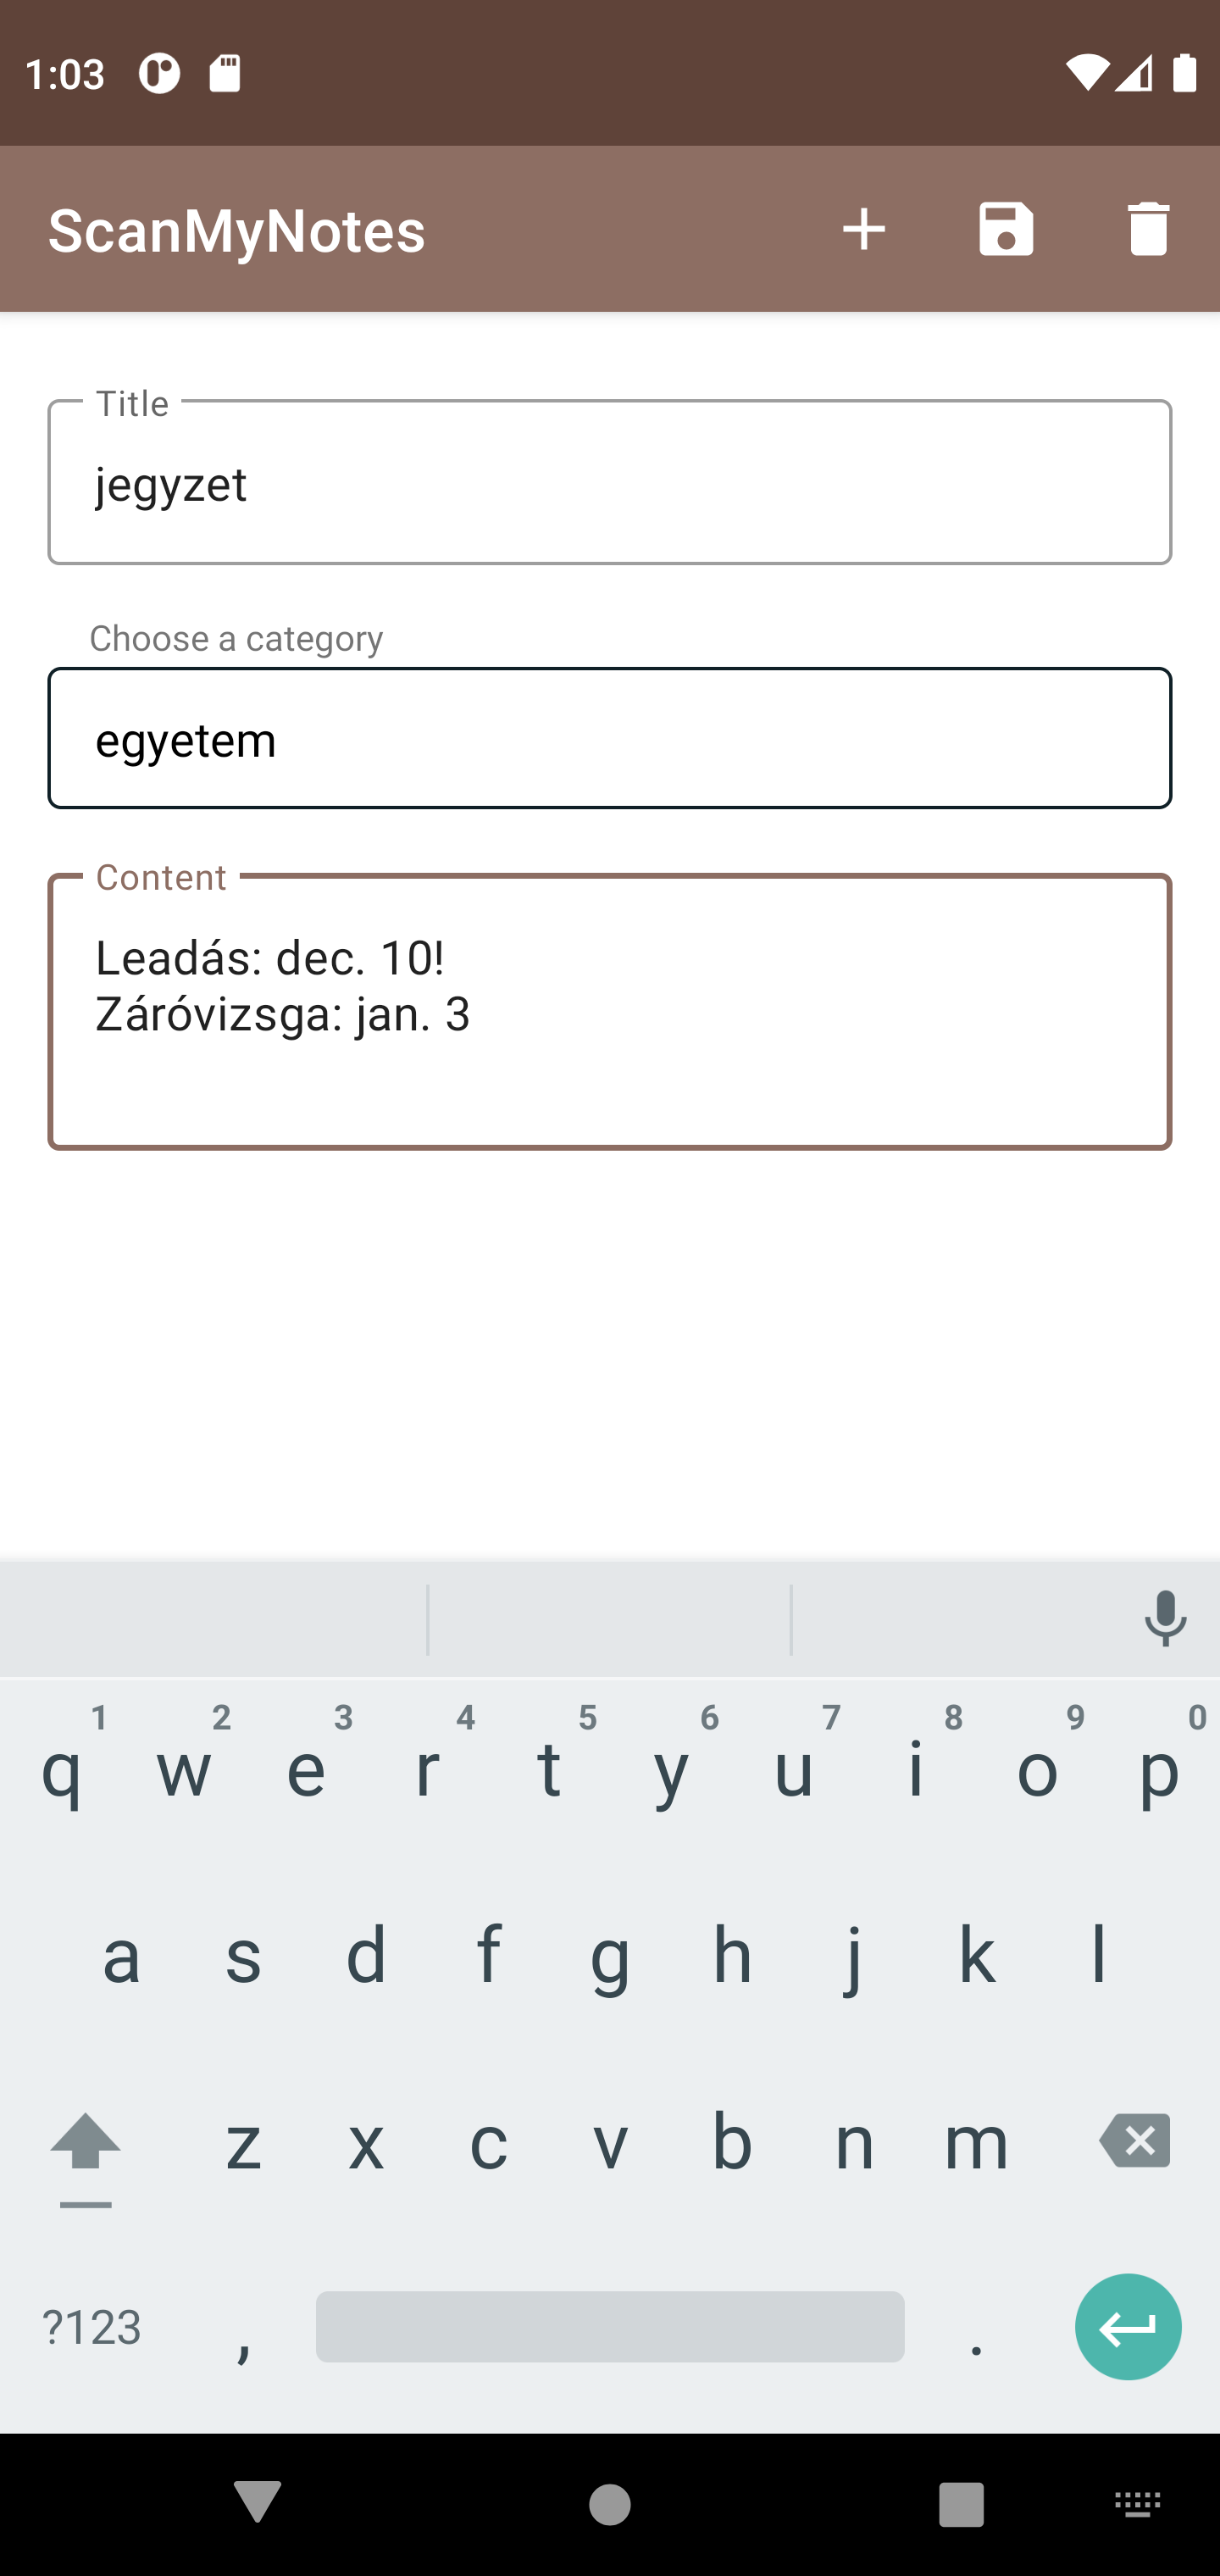
\includegraphics[width=55mm, keepaspectratio]{figures/note_edit.png}
	\caption{A jegyzet megtekintési, illetve szerkesztési képernyője.}
	\label{fig:NoteDetailsScreen}
\end{figure}
\newpage
\section{Kategória létrehozása}
Az alkalmazásban elérhető másik adattípus a kategória, mely rendszerezési célt szolgál. Képes magába foglalni jegyzeteket és más kategóriákat is, tetszőleges mélységben. Szintén a jobb alsó sarokban található gomb biztosítja a létrehozás lehetőségét, ám ebben az esetben a felugró két kisebb gomb közül a felsőt kell választani. Itt egy, a jegyzetkészítéshez nagyon hasonló oldalon tudunk címet és opcionálisan szülőkategóriát megadni, és amennyiben nem üres a cím mezője, el is menthetjük (\refstruc{fig:NewCategoryScreen}).

\begin{figure}[!ht]
	\centering
	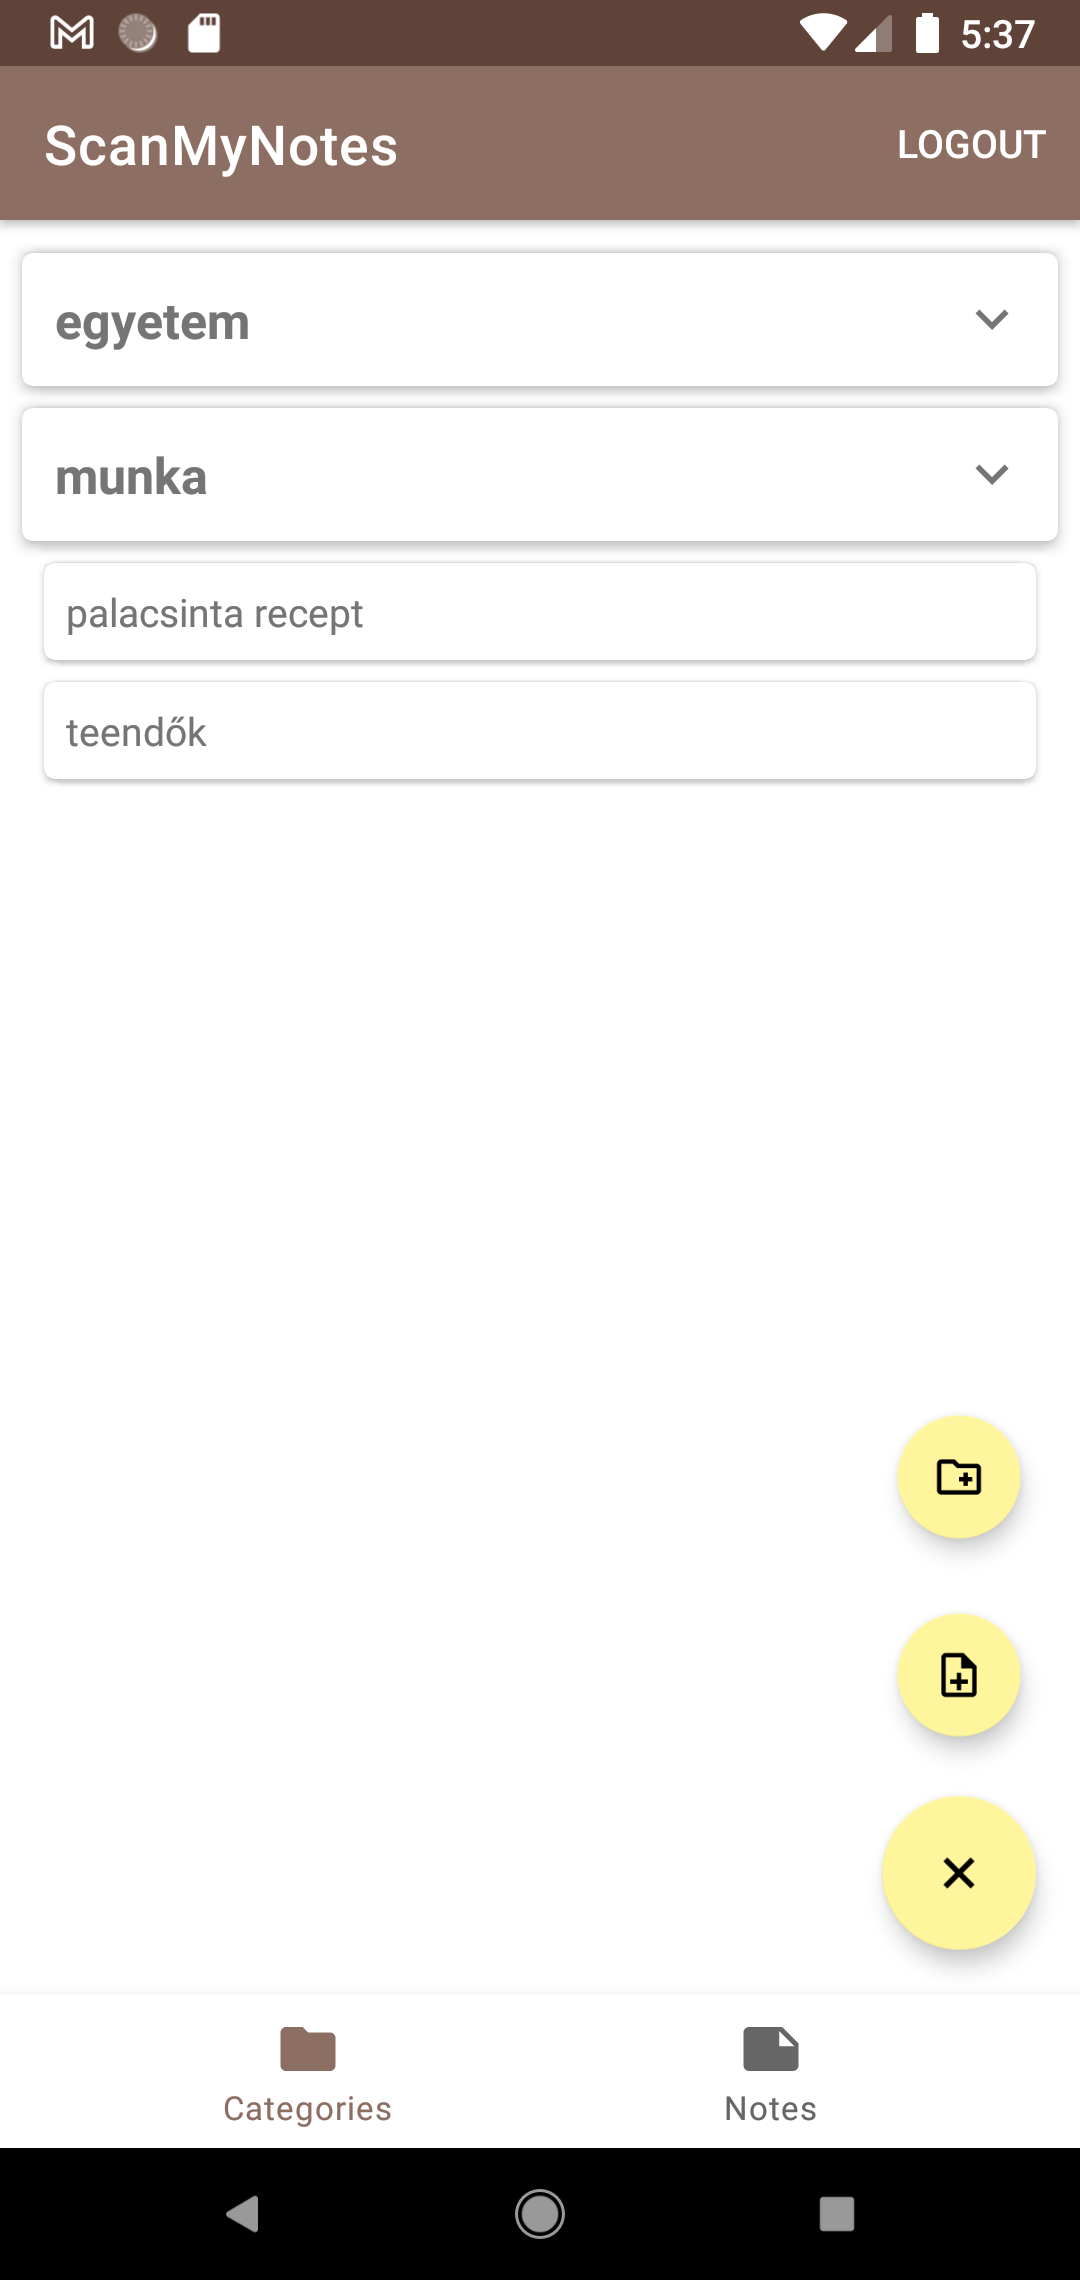
\includegraphics[width=55mm, keepaspectratio]{figures/floatingbutton_open.png}
	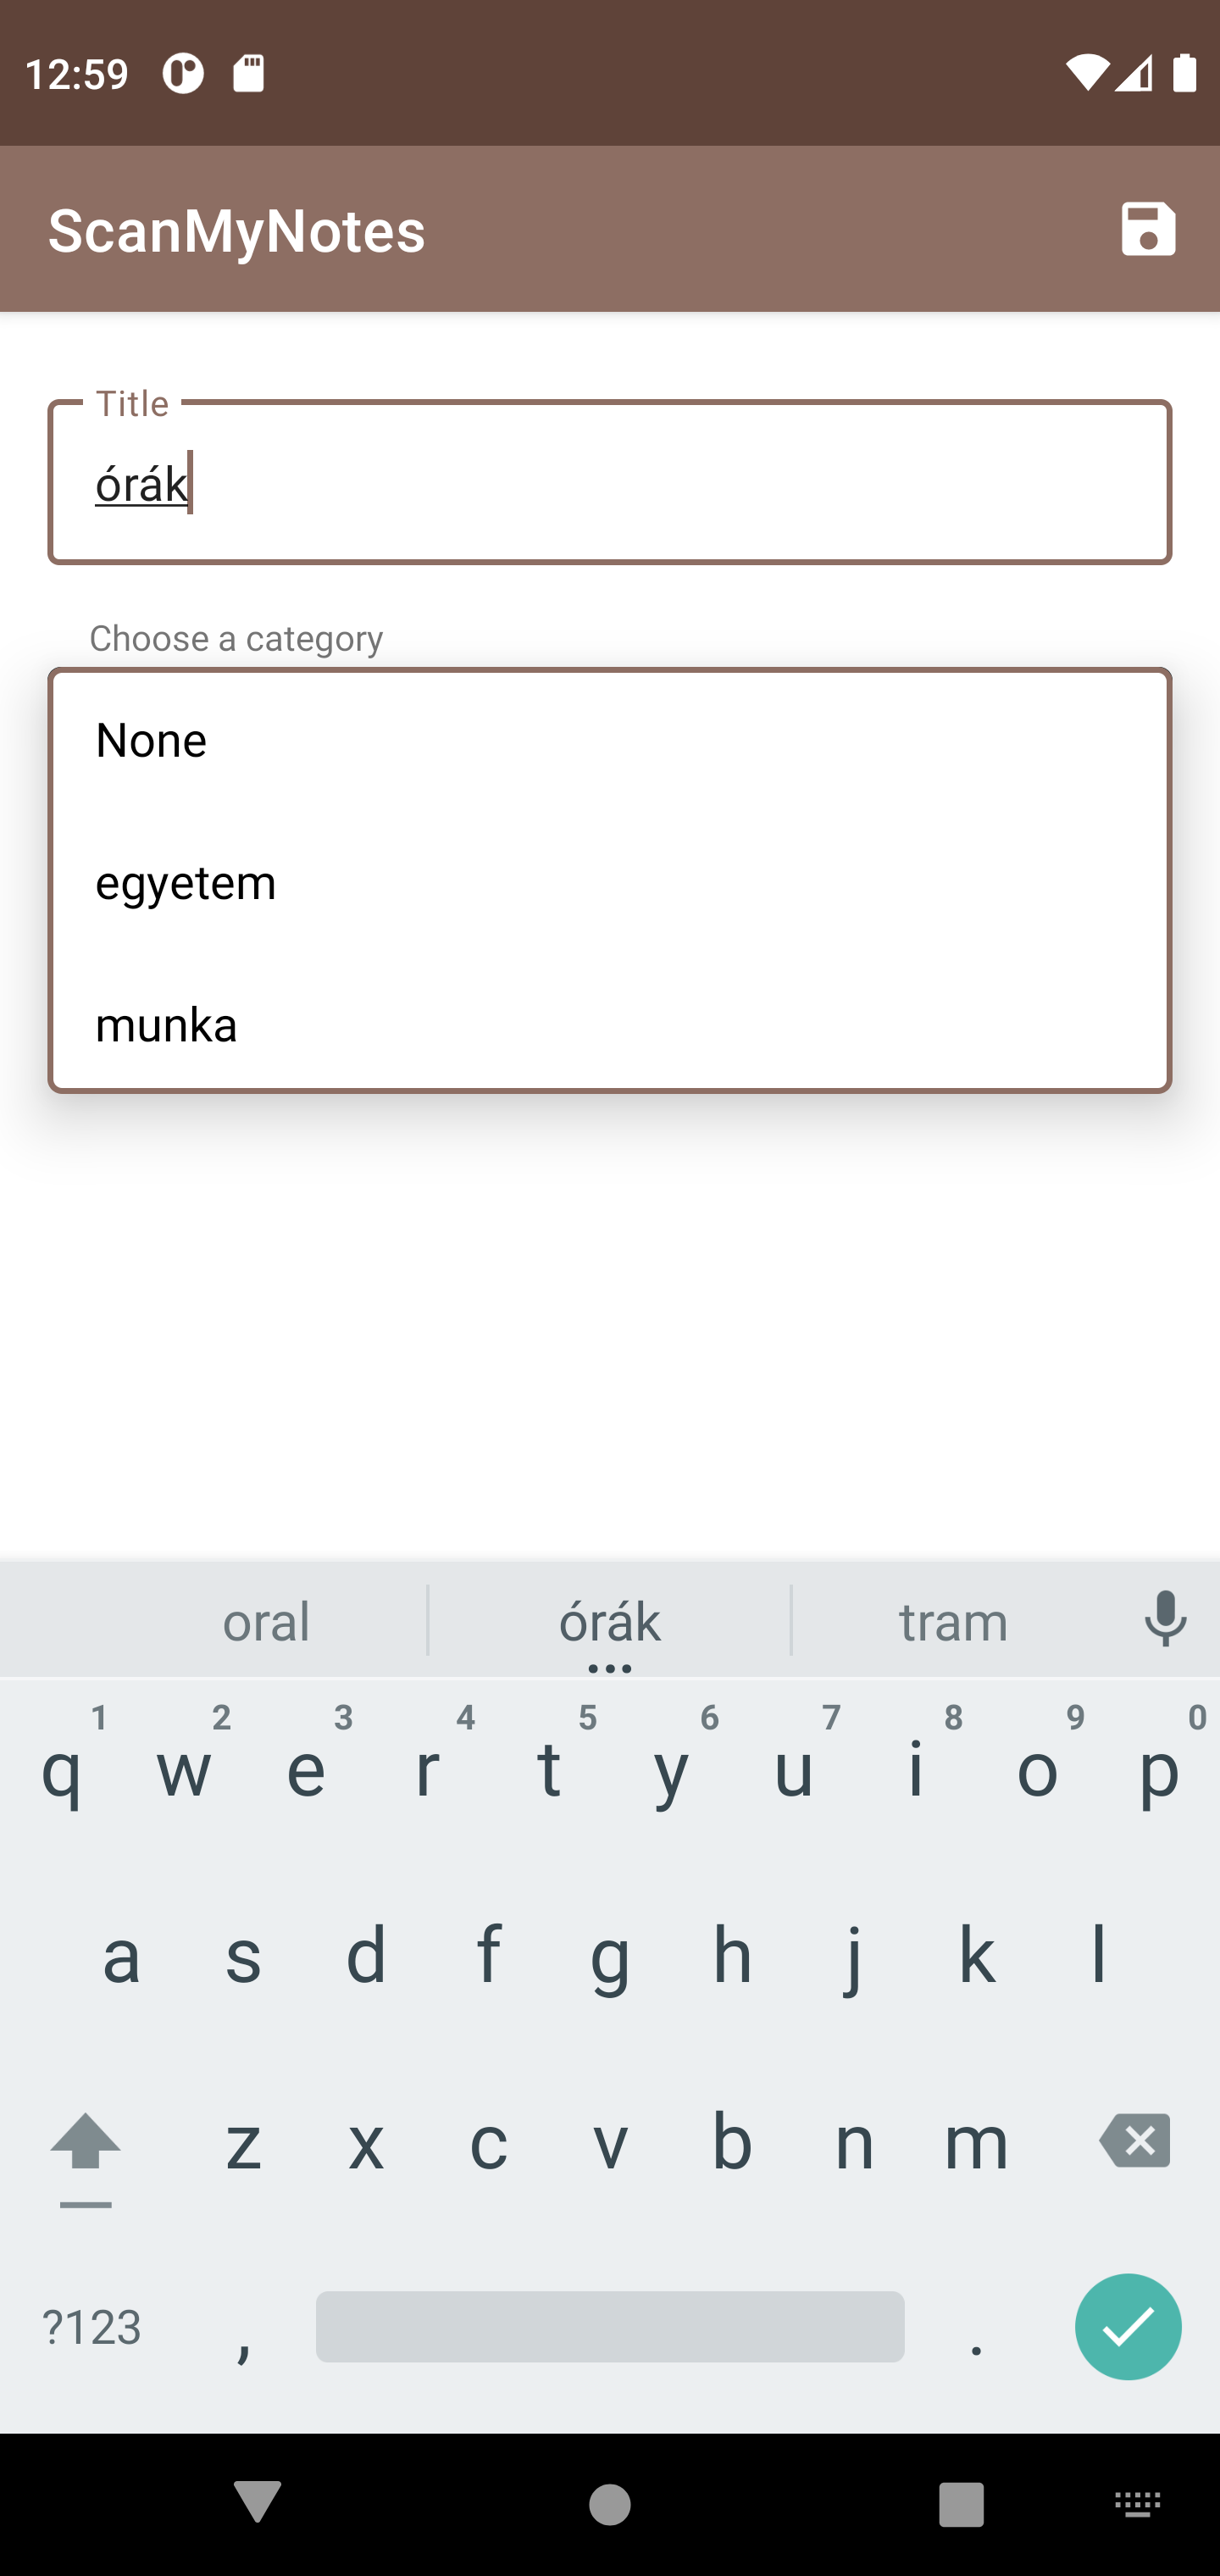
\includegraphics[width=55mm, keepaspectratio]{figures/category_save.png}
	\caption{A létrehozás gomb kinyitott állapotban, új kategória felvétele.}
	\label{fig:NewCategoryScreen}
\end{figure}
\newpage
\section{Kategória szerkesztése}
Új kategória létrehozása után, illetve a listában egy kategóriára nyomva annak részleteit tekinthetjük meg. Itt megjelenik a címe és esetleges szülője, és jobb fent szintén található egy ceruza ikon, mely lehetővé teszi a szerkesztést (\refstruc{fig:CategoryDetailsScreen}). Hasonlóan a jegyzethez megtekintés és szerkesztés során is törölhetjük az adott kategóriát, ilyenkor egy felugró ablak figyelmeztet rá, hogy a törlés során az összes tartalmazott objektum is törlődni fog.

\begin{figure}[!ht]
	\centering
	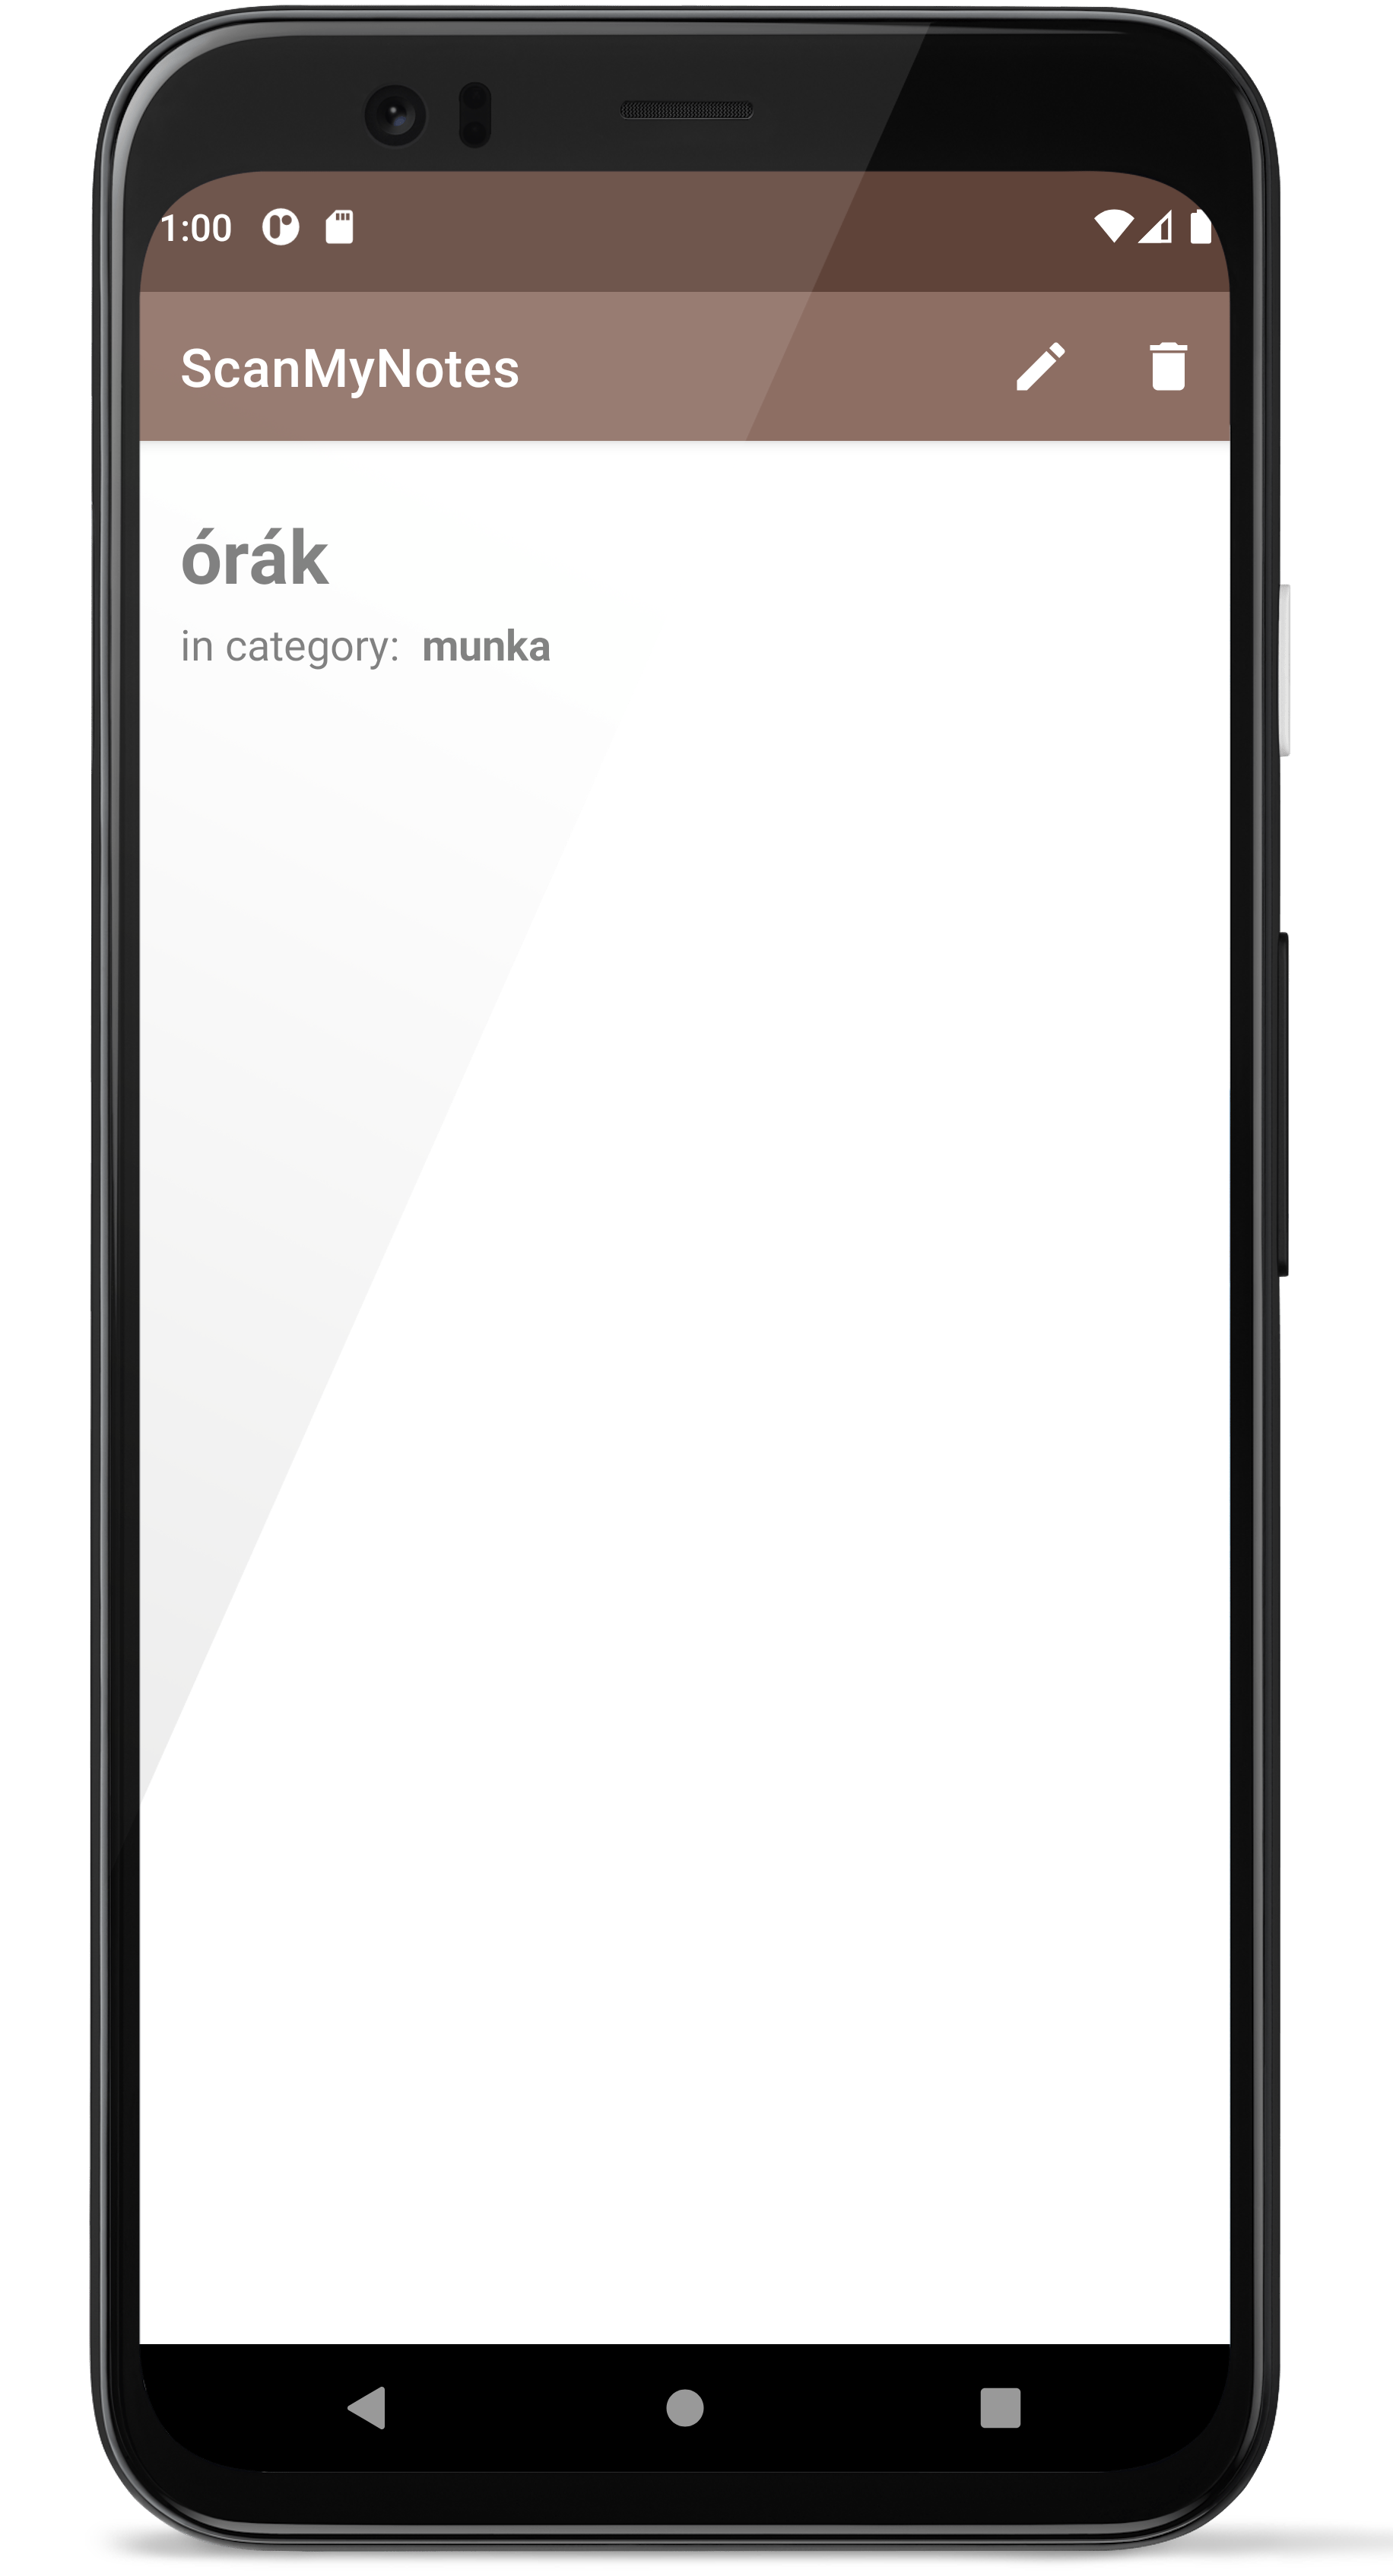
\includegraphics[width=55mm, keepaspectratio]{figures/category_view.png}
	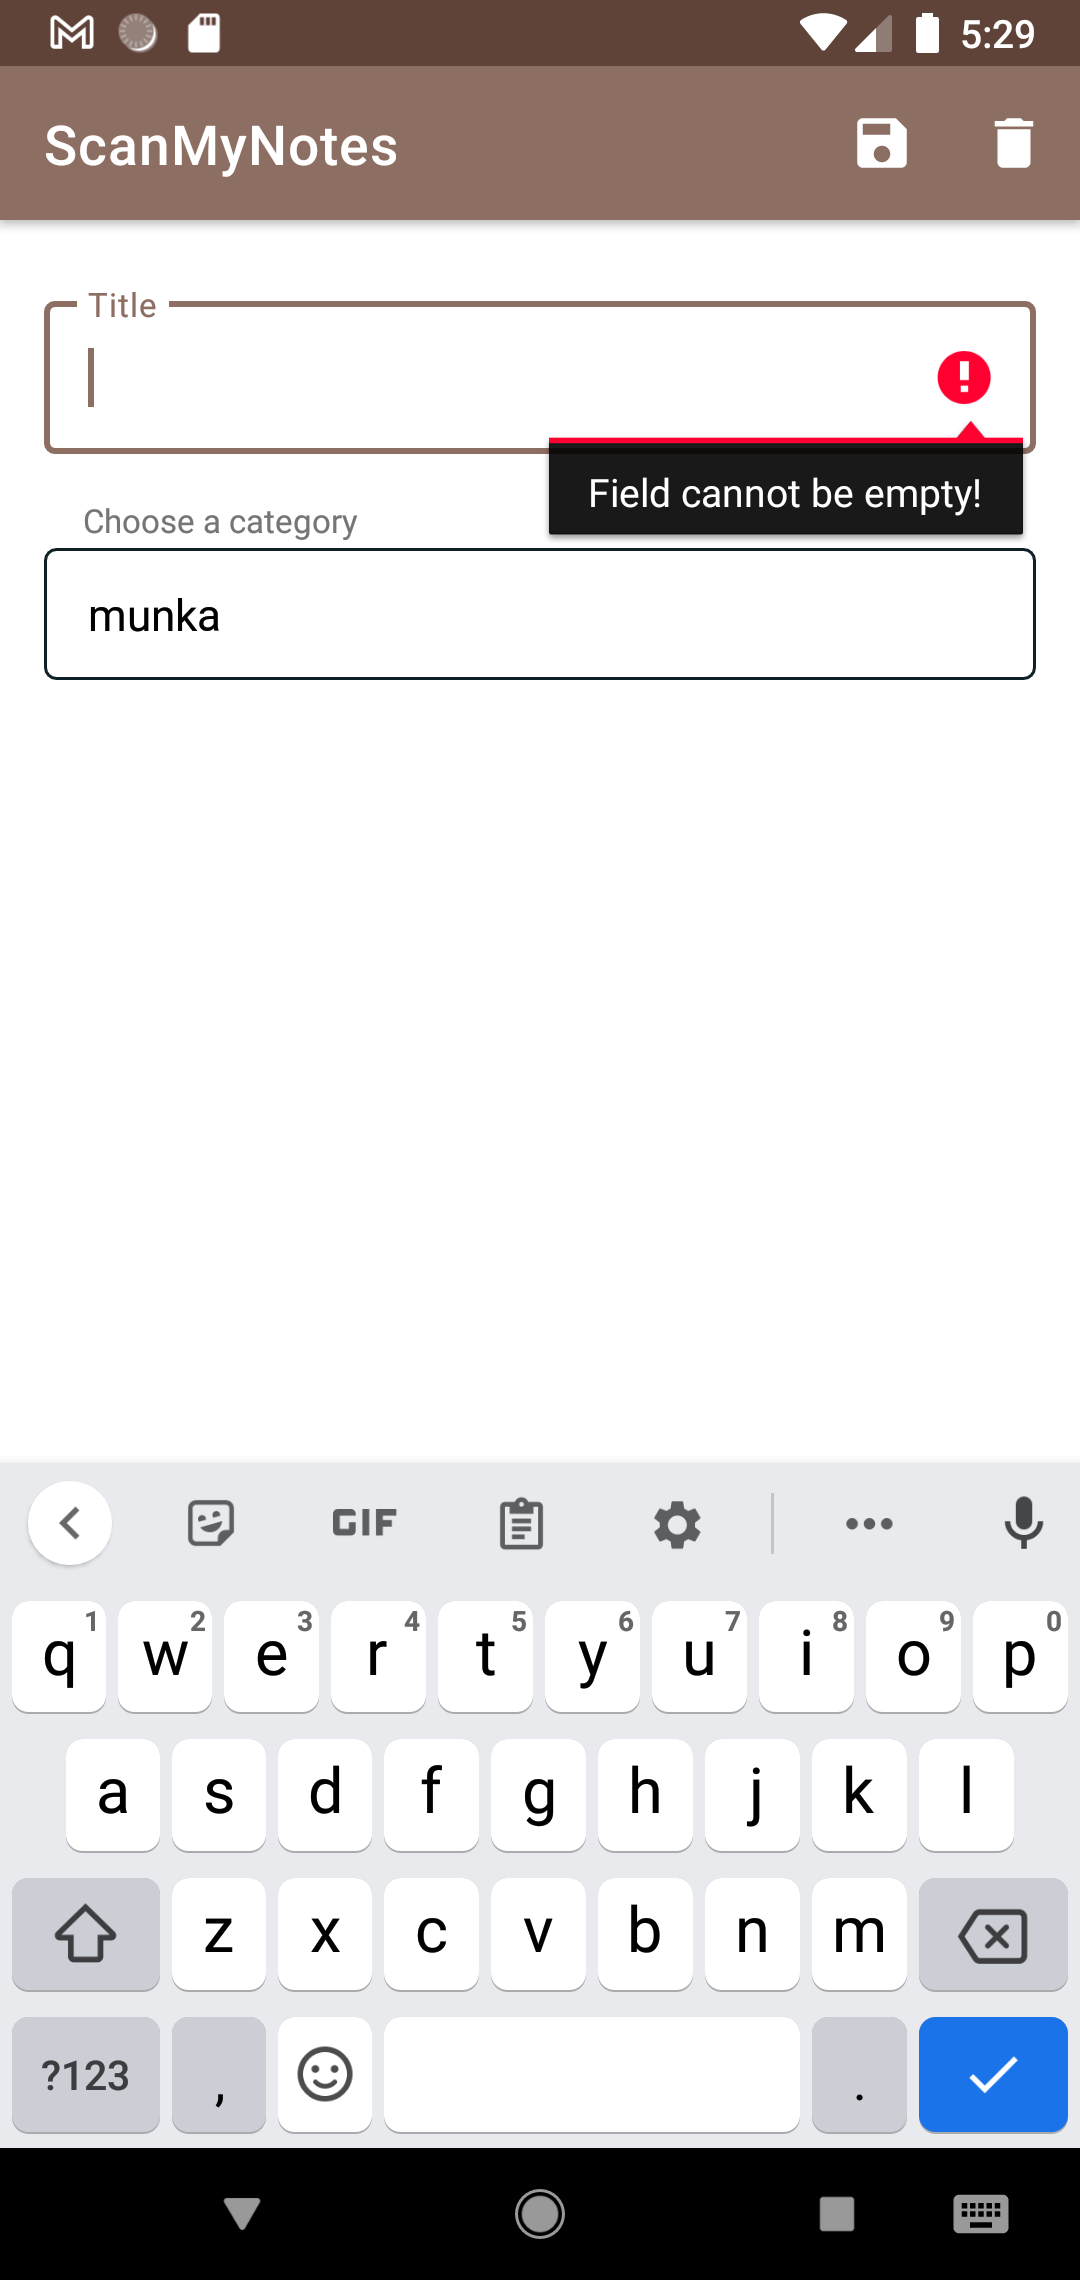
\includegraphics[width=55mm, keepaspectratio]{figures/category_edit_error.png}
	\caption{A kategória részletes képernyője, illetve a szerkesztési képernyő által feldobott hiba, ha üresen hagyjuk a címet.}
	\label{fig:CategoryDetailsScreen}
\end{figure}
%-----------------------
\chapter{Alkalmazás}
%-----------------------
%TODO write
%TODO spellcheck

Egy alkalmazás megvalósítása mindig komplex folyamat, mely sok kisebb részfolyamatot foglal magába. Az alábbiakban a fejlesztés részleteiről fogok írni, kezdve az alkalmazással szemben támasztott követelményekkel, majd képernyőképek segítségével bemutatom a működését. Ezután a megvalósítás részleteibe fogok belemenni, és végül a tesztelésről is ejtek pár szót.

\section{Követelmények}

A fejlesztés során alapvető célom volt egy, a modern paradigmáknak és a felhasználók elvárásainak megfelelő applikáció megalkotása. Törekedtem az objektumorientált szemlélet alkalmazására, a felelősségek szétválasztására és a maximális felhasználói élmény nyújtására. Fontos volt, hogy az alkalmazás folyamatai ne térjenek el nagymértékben attól, mint amit a felhasználók más applikációkban megszokhattak, és minden művelet meg legyen valósítva az adatokon, amire szükségük lehet. 

Ezek alapján az alábbi követelmények fogalmazódtak meg az alkalmazással szemben:
\begin{itemize}
	\item A felhasználónak legyen lehetősége fiókot létrehozni, e-mail cím és jelszó megadásával bejelentkezni, illetve fiókjából ki is lépni.
	\item Az adatok legyenek perzisztensen tárolva, az alkalmazás bezárásával, abból való kilépéssel vagy egy esetleges készülékcsere esetén sem veszhetnek el.
	\item Az adatok csak bejelentkezés után váljanak láthatóvá.
	\item A felhasználó képes legyen kategóriákat létrehozni a jegyzetek számára, ezeket akár tetszőleges mélységben más kategóriákba ágyazni.
	\item Legyen lehetőség jegyzetek létrehozására dokumentumok lefényképezése által. A digitalizált szöveg visszakapása után a jegyzet lehessen címmel ellátható, kategóriába sorolható és a tartalma szerkeszthető.
	\item Inkonzisztens adatok létrehozására ne adjon lehetőséget, a felhasználói input mindig legyen validálva.
	\item A jegyzeteken és kategóriákon lehessen minden fő műveletet - létrehozás, olvasás, módosítás, törlés - elvégezni, ezek során a felhasználói felület és az adatbázis maradjanak konzisztensek egymással.
	\item Módosítás során lehessen a jegyzetet újabb fényképek készítésével kiegészíteni, az ily módon digitalizált szöveg kerüljön hozzáfűzésre az eredeti tartalomhoz.
	\item A UI esztétikai és felhasználói élmény szempontjából legyen megfelelő, a hosszú ideig tartó folyamatokat jelezze a felhasználónak töltőképernyő segítségével. 
	\item A jegyzetek listája lehessen rendezhető és kereshető. 
\end{itemize}

\section{Megvalósítás}

A következőkben az alkalmazás implementációjába fogok részletesebben belemenni a projektfelépítéstől kezdve a logikán át a felhasználói felületig.

\subsection{Projektfelépítés}
A projekt elrendezése úgy lett kialakítva, hogy megfeleljen a konvencióknak, emellett a package-ek nevei egyértelműek legyenek és könnyedén meg lehessen találni bármit, amit keresünk. A felépítés a következő:
\begin{itemize}
	\item \emph{data:} Az adatelérési réteg osztályait tartalmazza, két package található benne: egy \emph{models} és egy \emph{network}. Előbbi a hálózati modell(eke)t tartalmazza, utóbbi pedig az API-kat és a DataSource-okat. 
	\item \emph{di:} Az architektúra ajánlása alapján ebbe a package-be kell tenni a függőséginjektálás működéséhez szükséges fájlokat.
	\item \emph{domain:} A domain réteg tartalmazza az üzleti logikát. Ez általában interactorokból és üzleti modellekből áll, jelen applikációban az egy darab interactort és a modelleket jelenti. 
	\item \emph{ui:} Ez tartalmazza a felhasználói felülethez kapcsolódó összes kódot, azaz itt találhatók a Fragmentek, ViewModelek, ViewState-ek, illetve egyéb, megjelenítéshez kapcsoló szükséges osztályok. 
	\item \emph{util:} Ide kerültek azok a dolgok, amiket máshova nem lehetett beilleszteni. Egyetlen fájl található benne, olyan kiegészítésekkel, amiket több osztály is használ, ezért nem lehetett egy funkcióhoz kötni.
\end{itemize}

\subsection{Szerveroldali komponensek integrációja}
Az alkalmazás backendjét a Firebase szolgáltatja, melynek kiterjedt és alapos dokumentációja nagyban megkönnyíti az integrációs folyamatot. 

Első lépésként be kell jelentkezni a Firebase console\footnote{\url{https://console.firebase.google.com/}}-ba, és létrehozni az alkalmazás számára egy Firebase projektet. Amikor kész, akkor ehhez hozzá kell adni a már létező applikációt azáltal, hogy megadjuk az alkalmazás package nevét\footnote{A package név egy egyedi azonosító, mely alapján egyértelműen meghatározható az alkalmazás. Két ugyanolyan package névvel rendelkező applikáció nem telepíthető fel egy eszközre, de még a Google Play Store-ba sem kerülhet.}. Ezután generálódik egy \emph{google-services.json} nevű fájl, melyet le kell tölteni, és a lokális projekt \emph{app} mappájába beilleszteni. A projekt szintű \emph{build.gradle} fájlba fel kell venni a Google Services Gradle plugint, mint függőséget, és ezt a modul szintű \emph{build.gradle} fájlban egy \emph{apply plugin} parancs felvételével alkalmazni kell. Végül pedig a használni kívánt Firebase szolgáltatásokat is fel kell venni függőségként az utóbbi fájlba, és egy gradle szinkronizálás után elérhetővé válnak az alkalmazásban.

A projektben négy Firebase szolgáltatás került felhasználásra, melyek az autentikáció, Firestore, Analytics és Crashlytics. Az alkalmazásban használt kódon kívül a menedzselésük a fentebb említett console-ban lehetséges, mely rendkívül kényelmes. Minden modul külön-külön be- és kikapcsolható a projekt igényeinek megfelelően, így az alkalmazás növekedésével később akár plusz funkciókat is bevezethetünk, mindössze egy kattintással. 

Az első szolgáltatás az Authentication, mely elég fontos aspektusa a működésnek. Bekapcsolás után számos lehetőség tárul elénk, de teljes mértékben miénk az irányítás: alapértelmezetten minden ki van kapcsolva, csak azt fogjuk tudni használni, amit mi magunk kapcsolunk be. A \emph{Sign-in method} fülre kattintva tudunk egy vagy több bejelentkezési módot választani, melyet az alkalmazásban használni szeretnénk. Támogatja az autentikációt e-mail és jelszó, telefonszám, Facebook, Google, Apple és GitHub használatával, és ezeken kívül még néhány módszerrel. A projektben az e-mail és jelszó kombinációját választottam, ugyanis ahhoz vannak a legjobban hozzászokva a felhasználók, az e-mail cím az, ami tényleg mindenkinek van, ellentétben egy Apple vagy egy Google fiókkal. Legalább egy bejelentkezési módot bekapcsolva pedig a \emph{Users} fülön láthatjuk a regisztrált felhasználók listáját (\refstruc{fig:AuthUsers})

\begin{figure}[!ht]
	\centering
	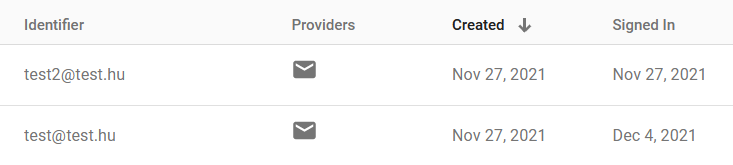
\includegraphics[width=100mm, keepaspectratio]{figures/auth_users.png}
	\caption{A regisztrált felhasználók listája.}
	\label{fig:AuthUsers}
\end{figure}

A bejelentkeztetést a \emph{ui.login} package-ben található \emph{LoginFragment} végzi. Ő a többi képernyővel ellentétben csak egy sima Fragment, nem a RainbowCake architektúra része, ugyanis tulajdonképpen két függvényből áll az egész, így nem tartottam célszerűnek végigvezetni a rétegeken. Ahogy azt a \refstruc{fig:MaterialBeforeAfter} korábban bemutatta, egyetlen képernyő áll rendelkezésre mind a bejelentkezéshez, mind a regisztrációhoz. Ez a döntés azért született meg, mert az alkalmazás jelenlegi funkcionalitásában nincs szerepe a felhasználói profilnak, nincs szükség semmilyen plusz információra a felhasználótól, ami később bármilyen formában felhasználásra kerülne, így felesleges két teljesen ugyanolyan UI-t készíteni csak a megkülönböztetés kedvéért.

Az autentikáció végrehajtásához a Firebase biztosít egy \emph{FirebaseAuth} típusú objektumot, melyen keresztül elérhető az összes ezzel kapcsolatos művelet. Meg lehet nézni, hogy van-e bejelentkezett felhasználó, és ezzel átugorható a bejelentkezési folyamat, ha valaki korábban már használta az alkalmazást. Ha nem, akkor pedig (e-mail és jelszavas bejelentkezés esetén) a \emph{signInWithEmailAndPassword} és a \emph{createUserWithEmailAndPassword} függvények állnak rendelkezésre, melyeknek az e-mail címet és a jelszót paraméterként megadva elvégzik a megfelelő műveletet. Az eredményt aszinkron módon küldi, amire egy \emph{onCompleteListener} segítségével lehet feliratkozni. Ezen belül ellenőrizhető a hívás kimenetele, és sikeres művelet esetén át tudunk navigálni az alkalmazás megfelelő képernyőjére, hiba esetén pedig kezelni tudjuk azt.

A következő szolgáltatás a Firestore, mely adatok felhőalapú tárolását teszi lehetővé egy hierarchikus struktúrában. Bekapcsolása után elérhetővé válik a kezelőfelülete, ahol szabályokat adhatunk meg a hozzáférésre, illetve láthatunk minden tárolt adatot egy könnyen átlátható vizuális reprezentációban. Az alkalmazás adatai az (\refstruc{fig:Firestore}) által mutatott módon kerülnek tárolásra. 

Az összes adat egy \emph{users} nevű kollekcióban található, amiben minden felhasználóhoz tartozik egy dokumentum, melynek neve a regisztrációkor generált UID. Mivel ez garantáltan egyéni, így mindenki csak a saját adatait fogja elérni, és nem fordulhat elő, hogy egy felhasználó tudtán kívül felülírja egy másik adatait. A felhasználók dokumentumai két kollekciót tárolnak: egyet a kategóriáknak, és egyet a jegyzeteknek. Ezeken belül egy-egy dokumentum tárol egy-egy jegyzetet illetve kategóriát, melyeknek szintén egyéni azonosítója van. 

Az alkalmazásban a \emph{data.network} package-ben található \emph{FirebaseApi} nevű osztály végzi az adatok lekérését és objektumokká való konvertálását. Az adatbázist egy \emph{FirebaseFirestore} típusú objektumon keresztül érem el, a \refstruc{fig:FirestoreQuery} által mutatott kóddal. 

\begin{figure}[!ht]
	\centering
	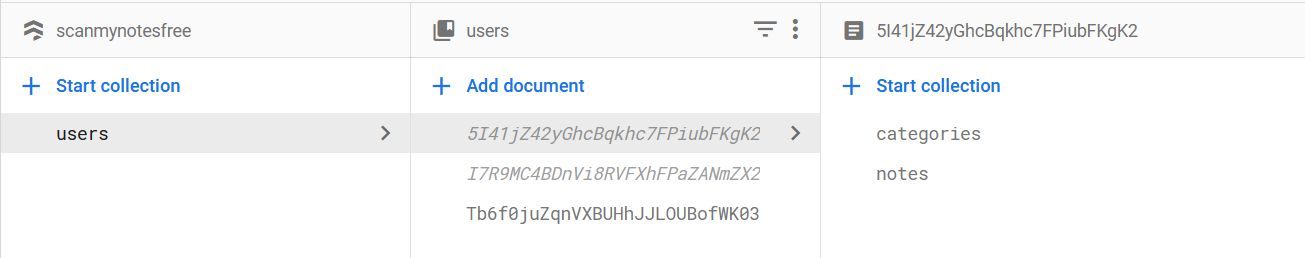
\includegraphics[width=150mm, keepaspectratio]{figures/firestore.png}
	\caption{A felhasználók adatainak struktúrája.}
	\label{fig:Firestore}
\end{figure}

\begin{figure}[!ht]
	\centering
	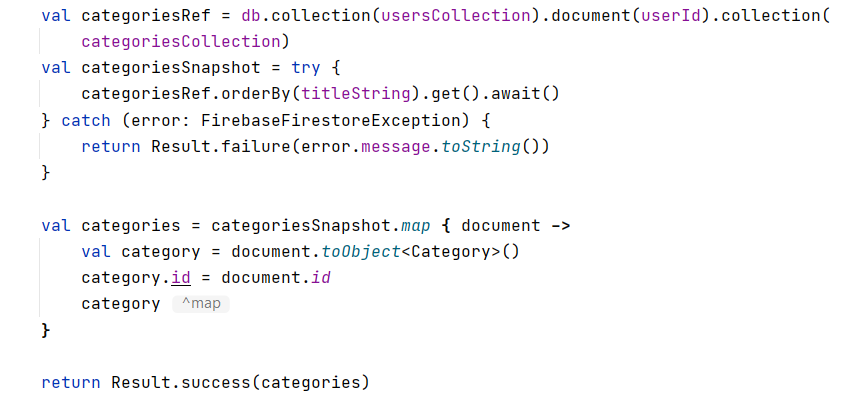
\includegraphics[width=150mm, keepaspectratio]{figures/firestore_query.png}
	\caption{A kategóriák lekérésének kódja az adatbázisból.}
	\label{fig:FirestoreQuery}
\end{figure}

Itt a \emph{db} változó az a bizonyos objektum, melyen keresztül elérhető az adatbázis. A hívástól függően egy \emph{CollectionReference} vagy egy \emph{DocumentReference} lehet az eredmény, ami az adott kollekció/dokumentum helyére mutat. Ezek felhasználhatók adatok írására és olvasására, ha pedig nem létezik adat azon a helyen, akkor létrehozza azt. Alapértelmezetten a referenciákon végzett minden hívás aszinkron módon hajtódik végre, de ez a működés nem volt ideális az alkalmazásom számára, ezért a \emph{kotlinx.coroutines.tasks.await()} függvény segítségével bevárom a lekérdezés eredményét. Ezután már csak annyi van hátra, hogy a visszakapott Snapshot objektumból kialakítsam azokat a típusokat, amikre szüksége van az alkalmazásnak. Szerencsére ez rendkívül egyszerű, mivel a Firestore biztosít egy \emph{toObject} függvényt, melynek a kívánt típust template-paraméterként megadva elvégzi a konverziót. Az id-t pedig azért kell még utána beállítani a kapott objektumon, mert az nem egy tárolt mezője a dokumentumnak, hanem az azonosítója, így arra nem terjed ki a \emph{toObject}.

A harmadik szolgáltatás az Analytics, mely rengeteg hasznos információt szolgáltat a felhasználókról és szokásaikról. Az előzőekhez hasonlóan itt is egy objektum biztosítja a kívánt funkcionalitást, melynek típusa ez esetben \emph{FirebaseAnalytics}. Ez figyel pár darab beépített eseményt, mint például a képernyők látogatását vagy a munkamenet-kezdést, de sajátot is lehet definiálni (\refstruc{fig:Analytics}). Itt egy új felhasználó regisztrációját rögzíti a rendszer annak metódusával együtt, ami jelen esetben e-mail és jelszó. 

\begin{figure}[!ht]
	\centering
	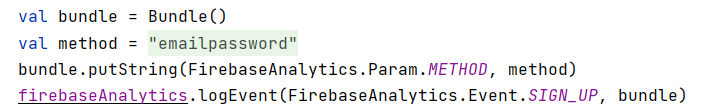
\includegraphics[width=120mm, keepaspectratio]{figures/analytics_custom.png}
	\caption{Egyéni esemény létrehozása és logolása Analytics segítségével.}
	\label{fig:Analytics}
\end{figure}

Az utolsó Firebase szolgáltatás, amit az alkalmazásban felhasználtam, a Crashlytics. Az előzőektől ellentétben az első bekezdésben leírtakon kívül ennél még szükség van további integrációs lépésekre is a működéshez. Van ugyanis egy saját pluginja, amit a fentiekkel megegyező módon fel kell venni mindkét gradle fájlba. Ezt követően szükség van egy teszt crash előidézésére, majd az alkalmazás újraindítására, hogy az elküldhesse a hibajelentést a Crashlyticsnek. Ezt követően viszont nincs már szükség semmi másra, a kódba sem szükséges semmit felvenni, mert automatikusan figyeli az alkalmazást. Természetesen számos lehetőségünk van finomhangolni a működését egyéni kulcsok hozzáadásával, de akár a nem-végzetes hibák figyelésével is.

\subsection{Képfelismerés integrációja}

\subsection{Modellek elkészítése} 

\subsection{Összetett lista}

\subsection{Navigáció}

\section{Működés}

A következőkben az alkalmazás funkcióit fogom bemutatni, a leírásokat képernyőképekkel kiegészítve. A képek néhol eltérnek egymástól, melynek oka hogy az applikáció funkcionalitásából fakadóan nem volt lehetséges mindet az emulátoron elkészíteni, hanem a jegyzetek készítéséhez fizikai készülékre is szükség volt.

\subsection{Bejelentkezés}
A telepítést követően a bejelentkezési képernyő az első, amivel a felhasználó találkozik. Ez már korábban megjelent a dolgozatban, a \refstruc{fig:MaterialBeforeAfter} bemutatásában. Itt a beviteli mezők segédszövegei egyértelműsítik, hogy milyen adatok elvártak a bejelentkezéshez illetve regisztrációhoz. Ezek gombnyomás hatására validálásra kerülnek, és amennyiben az e-mail formátuma nem érvényes vagy a jelszó hossza nem éri el a 6 karaktert, akkor a folyamat meghiúsul, és a felhasználó értesül róla, hogy mely mező(k) tartalmát kell javítania. 
%TODO picture if short on pages

\subsection{Kategorizált lista}
Sikeres bejelentkezést követően az alkalmazás a fő képernyőjére navigál, ahol az eddig elmentett jegyzeteket láthatjuk kategóriákba rendezve. A kategóriák alapértelmezetten össze vannak csukva, csak a legfelső szinten található elemeket látjuk. A lista sorainak jobb szélén elhelyezkedő nyilakra kattintva tudjuk kibontani az adott kategóriát, ezzel megtekinteni a tartalmát (\refstruc{fig:NoteListScreen}).

\begin{figure}[!ht]
	\centering
	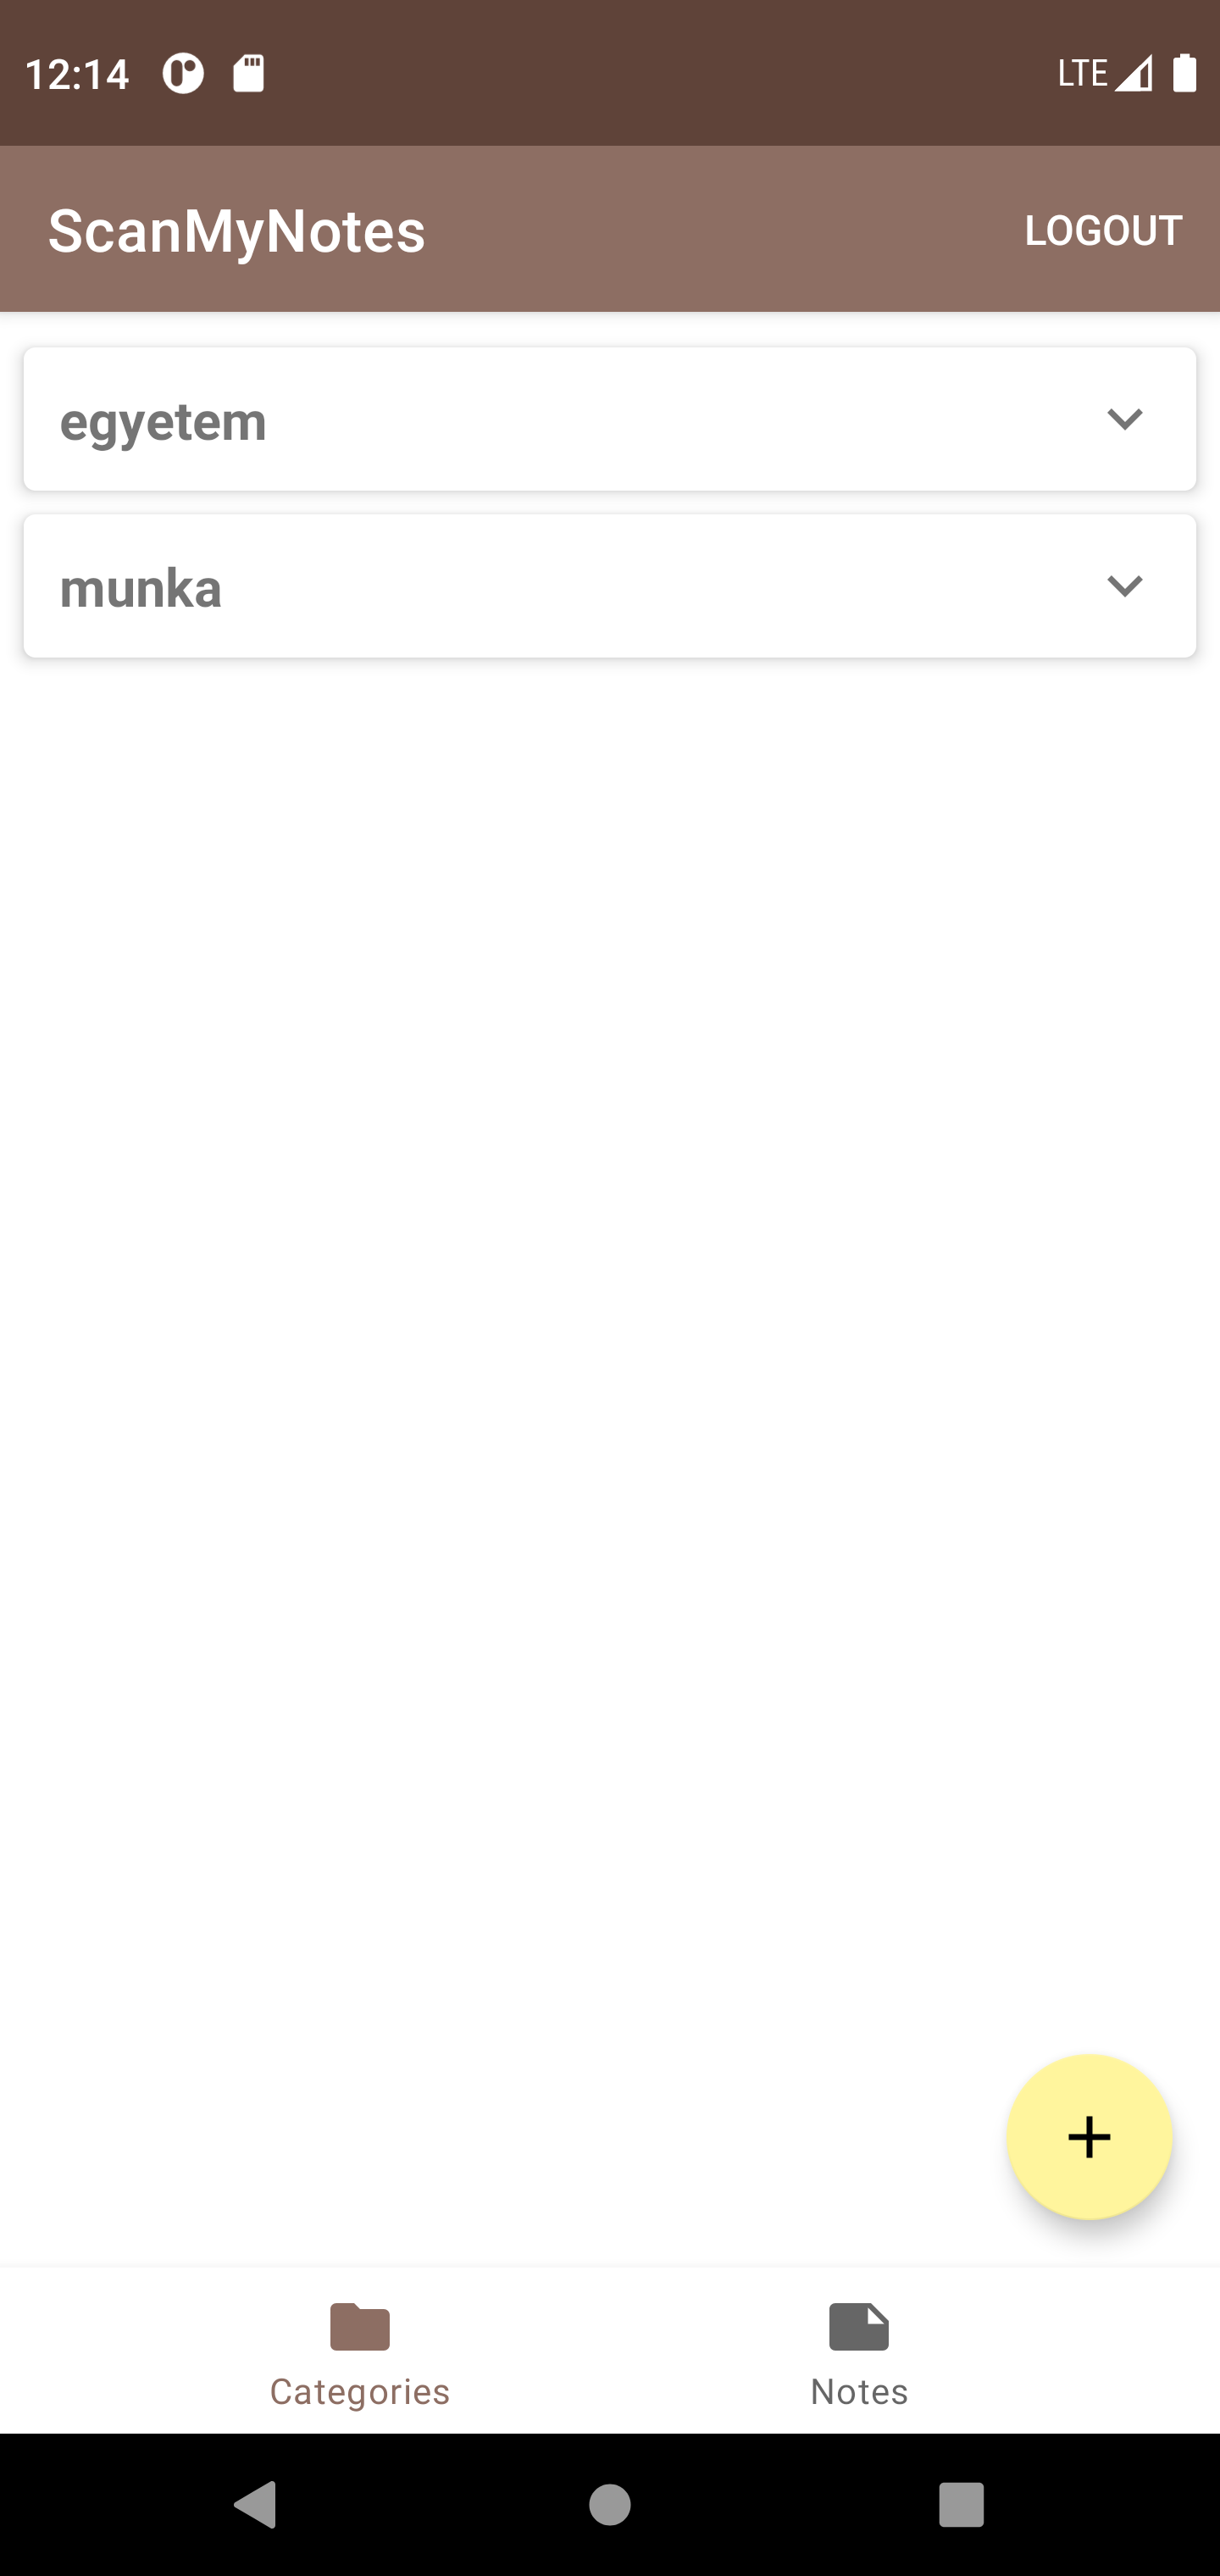
\includegraphics[width=55mm, keepaspectratio]{figures/notelist_closed.png}
	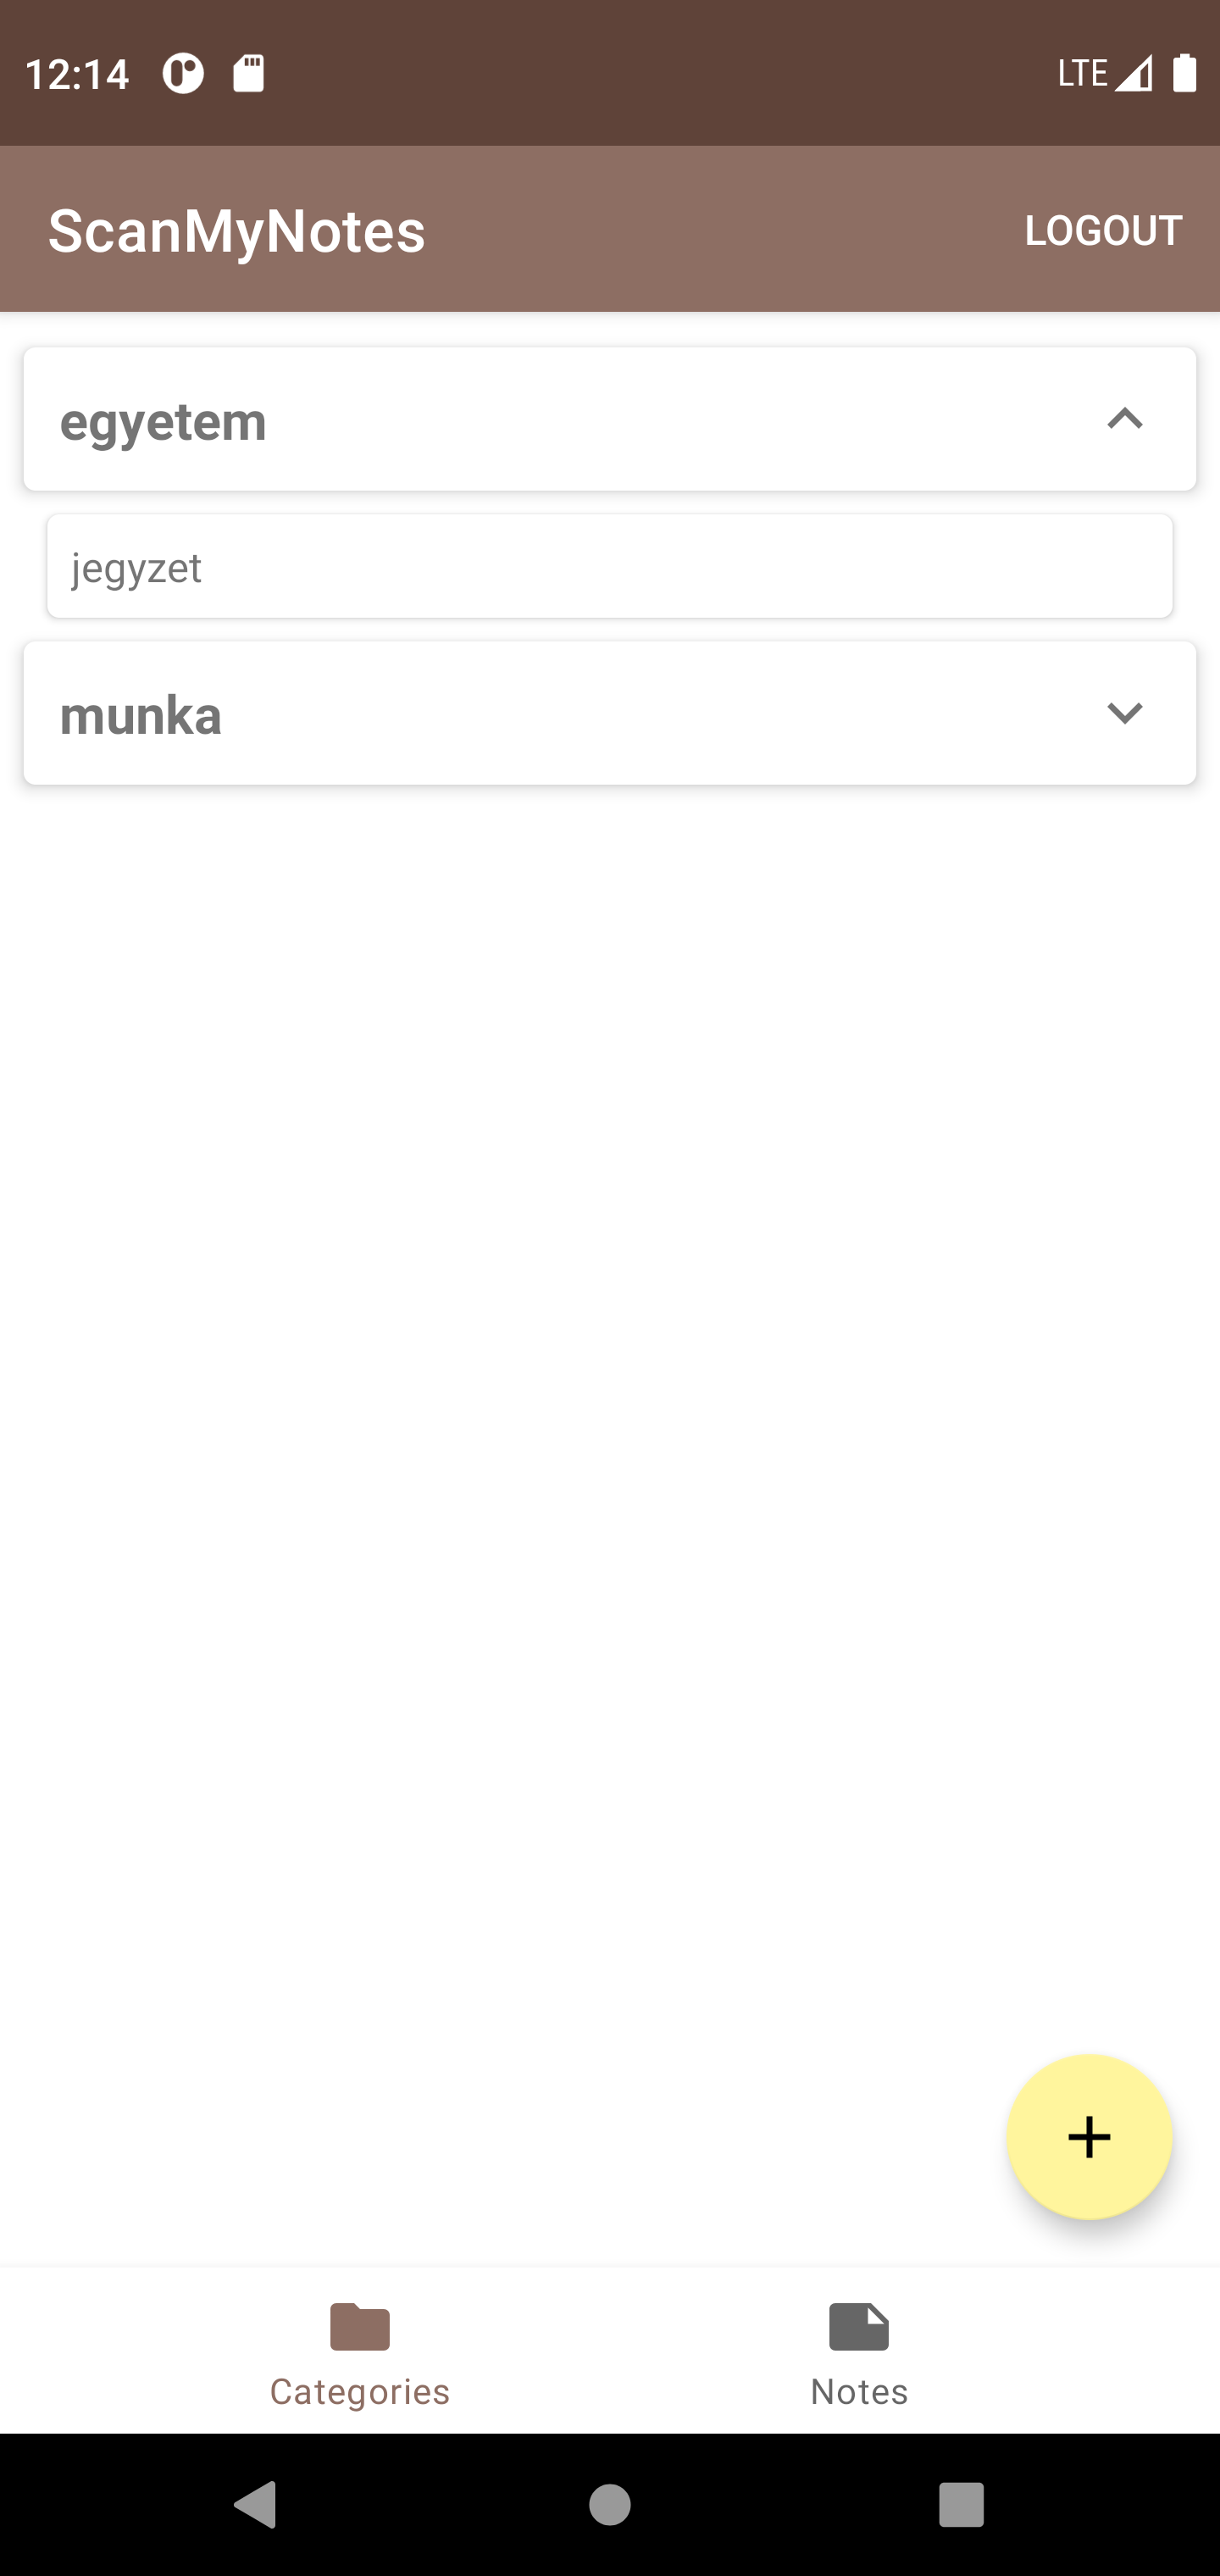
\includegraphics[width=55mm, keepaspectratio]{figures/notelist_open.png}
	\caption{Az alkalmazás kezdőlapja alapértelmezett állapotban, illetve egy kategória kibontva.}
	\label{fig:NoteListScreen}
\end{figure}

Innen számos lehetőségünk adódik navigációra az applikáción belül, kezdve a jobb felső sarokban található, meglehetősen magától értetődő kijelentkezés gombbal. Ezt megnyomva a fent leírt bejelentkezési képernyőre navigálunk, ahol adataink megadásával újra bejelentkezhetünk.

\subsection{Jegyzetlista}
A főképernyőn alul egy navigációs sávot találunk, mellyel a két különböző listamegjelenítés között tudunk váltani. Míg a \emph{Categories} opció alatt egy hierarchikusan egymás alá rendezett listát láthatunk, a \emph{Notes} opció csak a jegyzeteket tárja elénk, kategóriától függetlenül. Itt több lehetőség tárul elénk: a képernyő tetején található egy keresősáv és egy rendezés gomb. Keresni a jegyzetek címe alapján tudunk, itt gépelés közben azonnal szűkül az eredményhalmaz. A rendezés szintén a cím alapján működik, jelenleg növekvő és csökkenő betűrendet támogat az alkalmazás (\refstruc{fig:NoteListScreen2}). 

\begin{figure}[!ht]
	\centering
	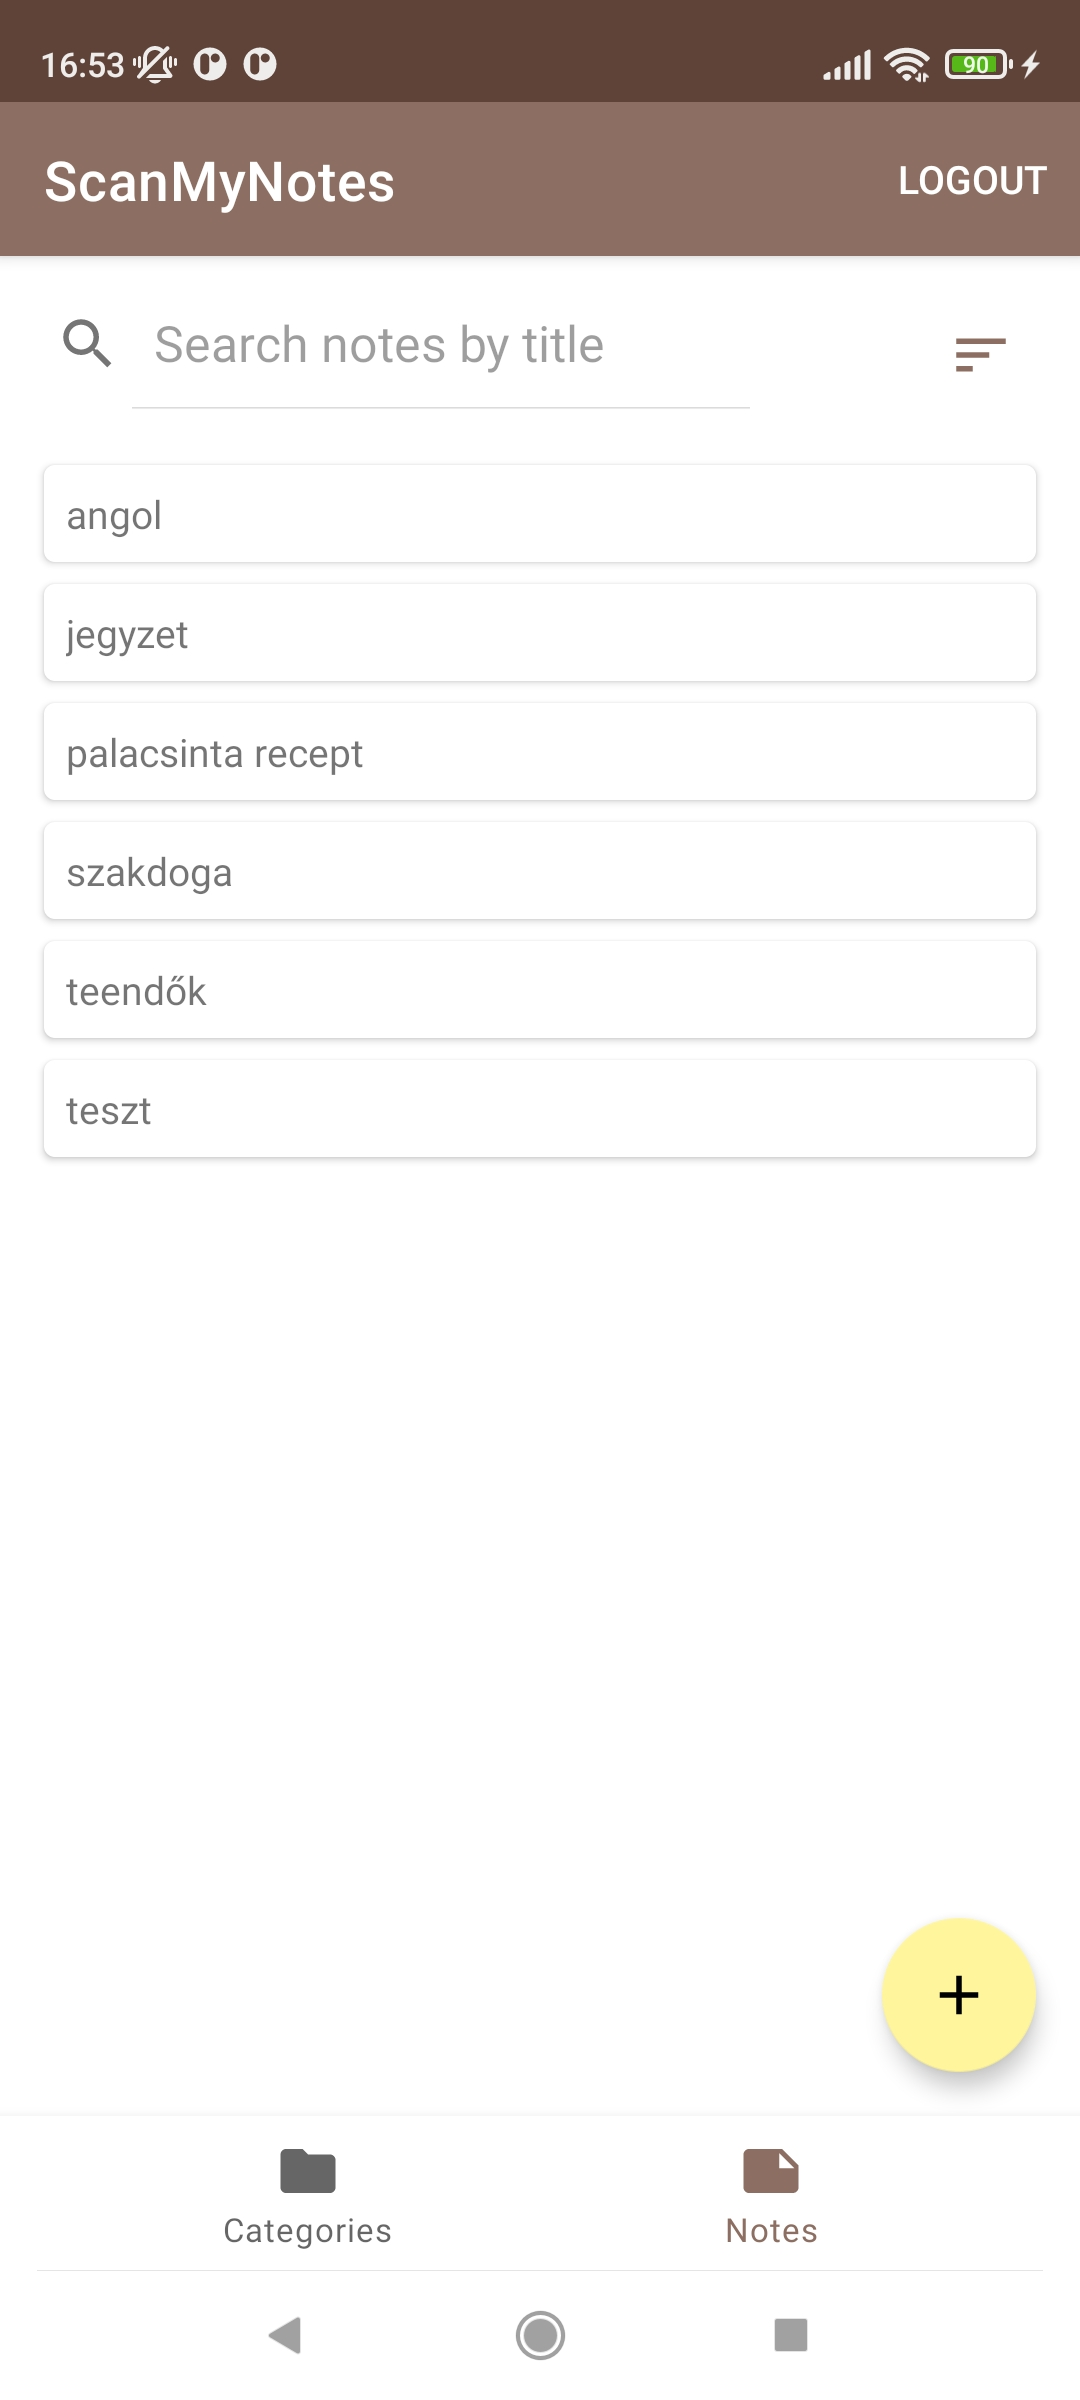
\includegraphics[width=49mm, keepaspectratio]{figures/notelist_full.jpg}
	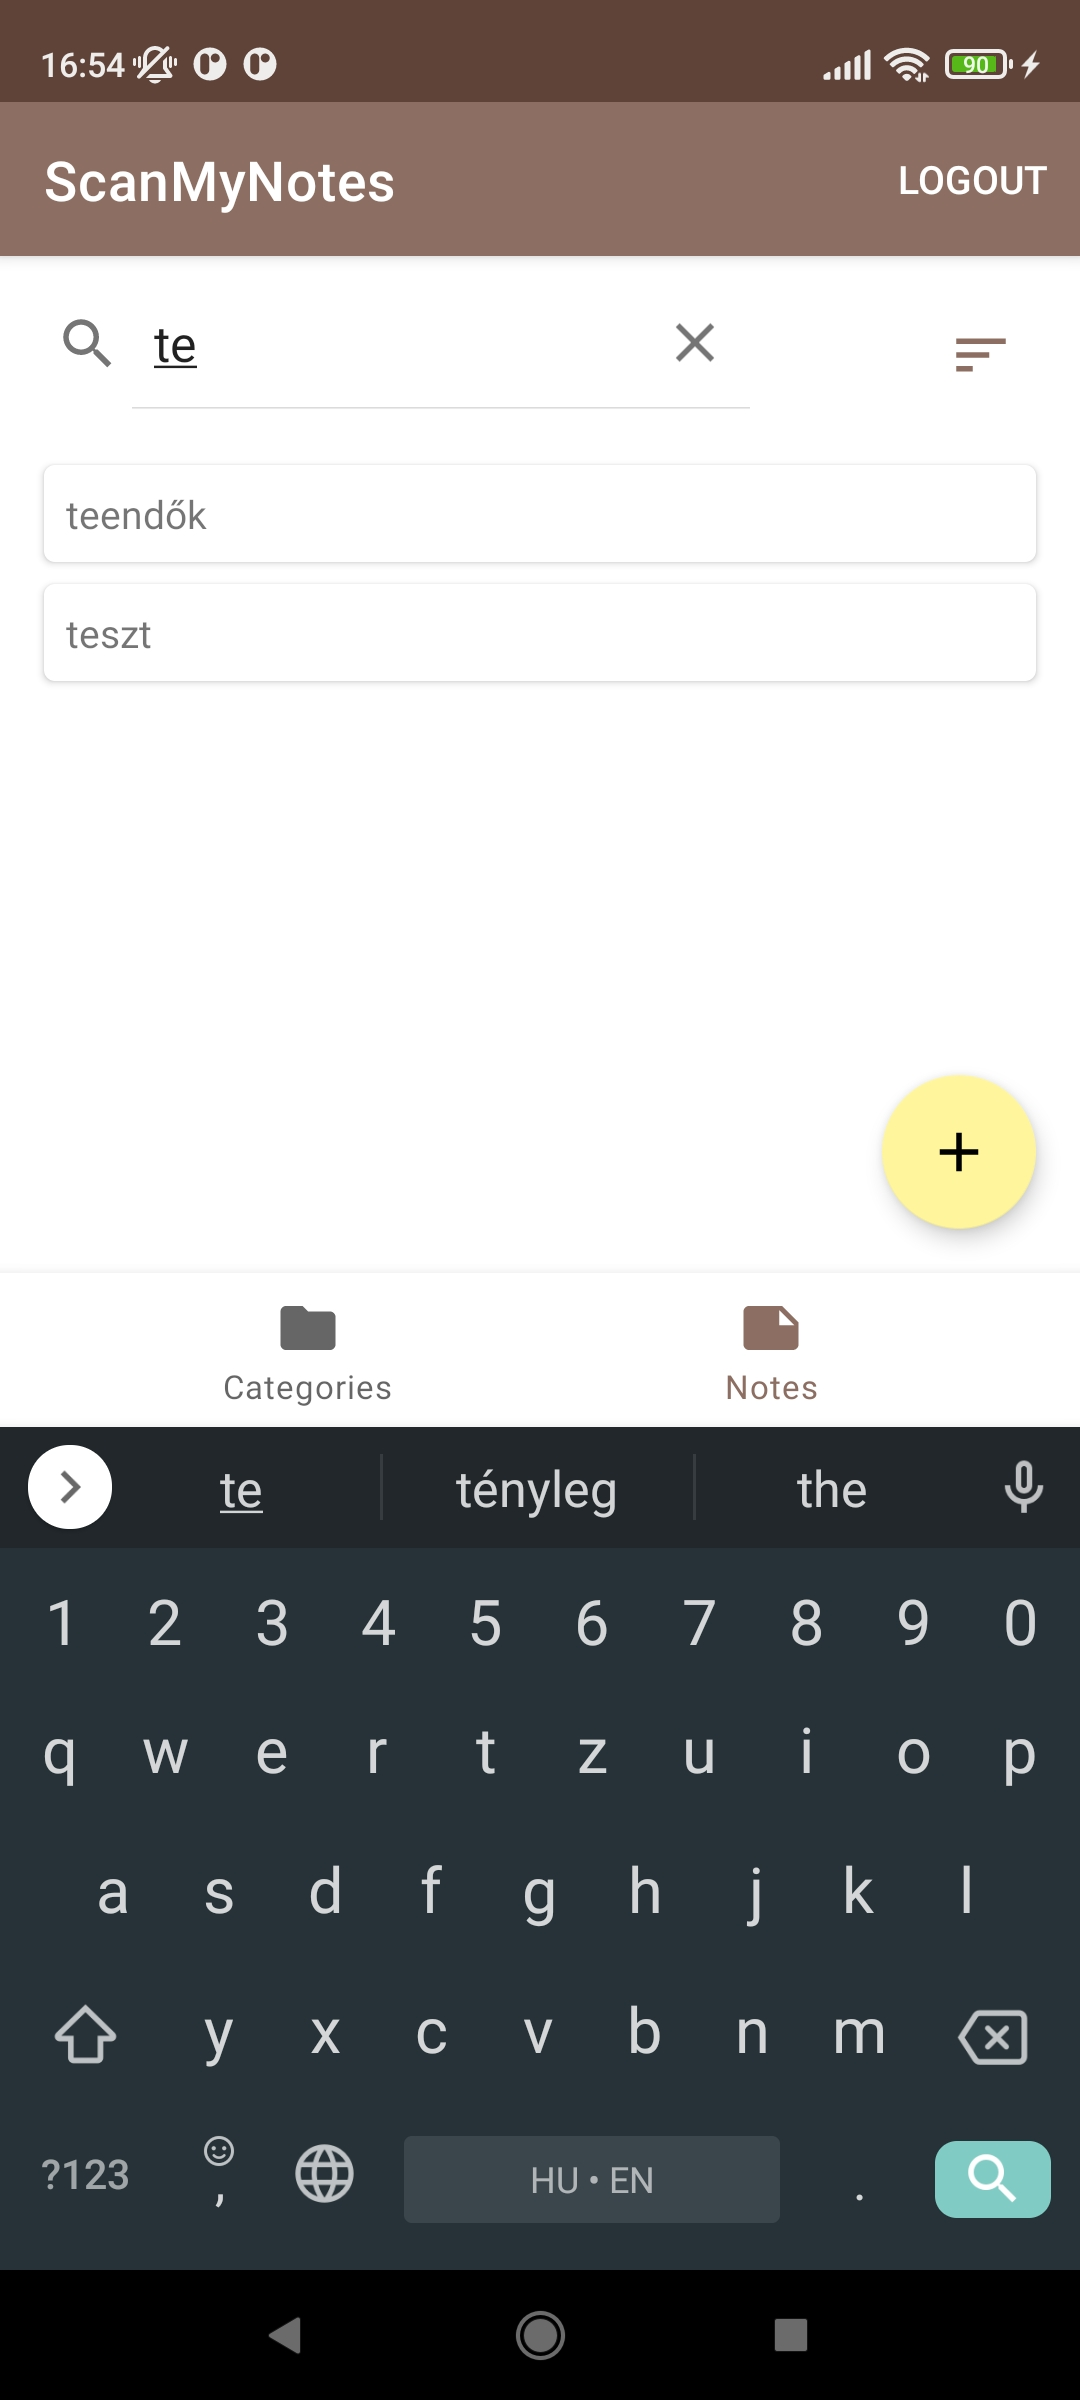
\includegraphics[width=49mm, keepaspectratio]{figures/notelist_search.jpg}
	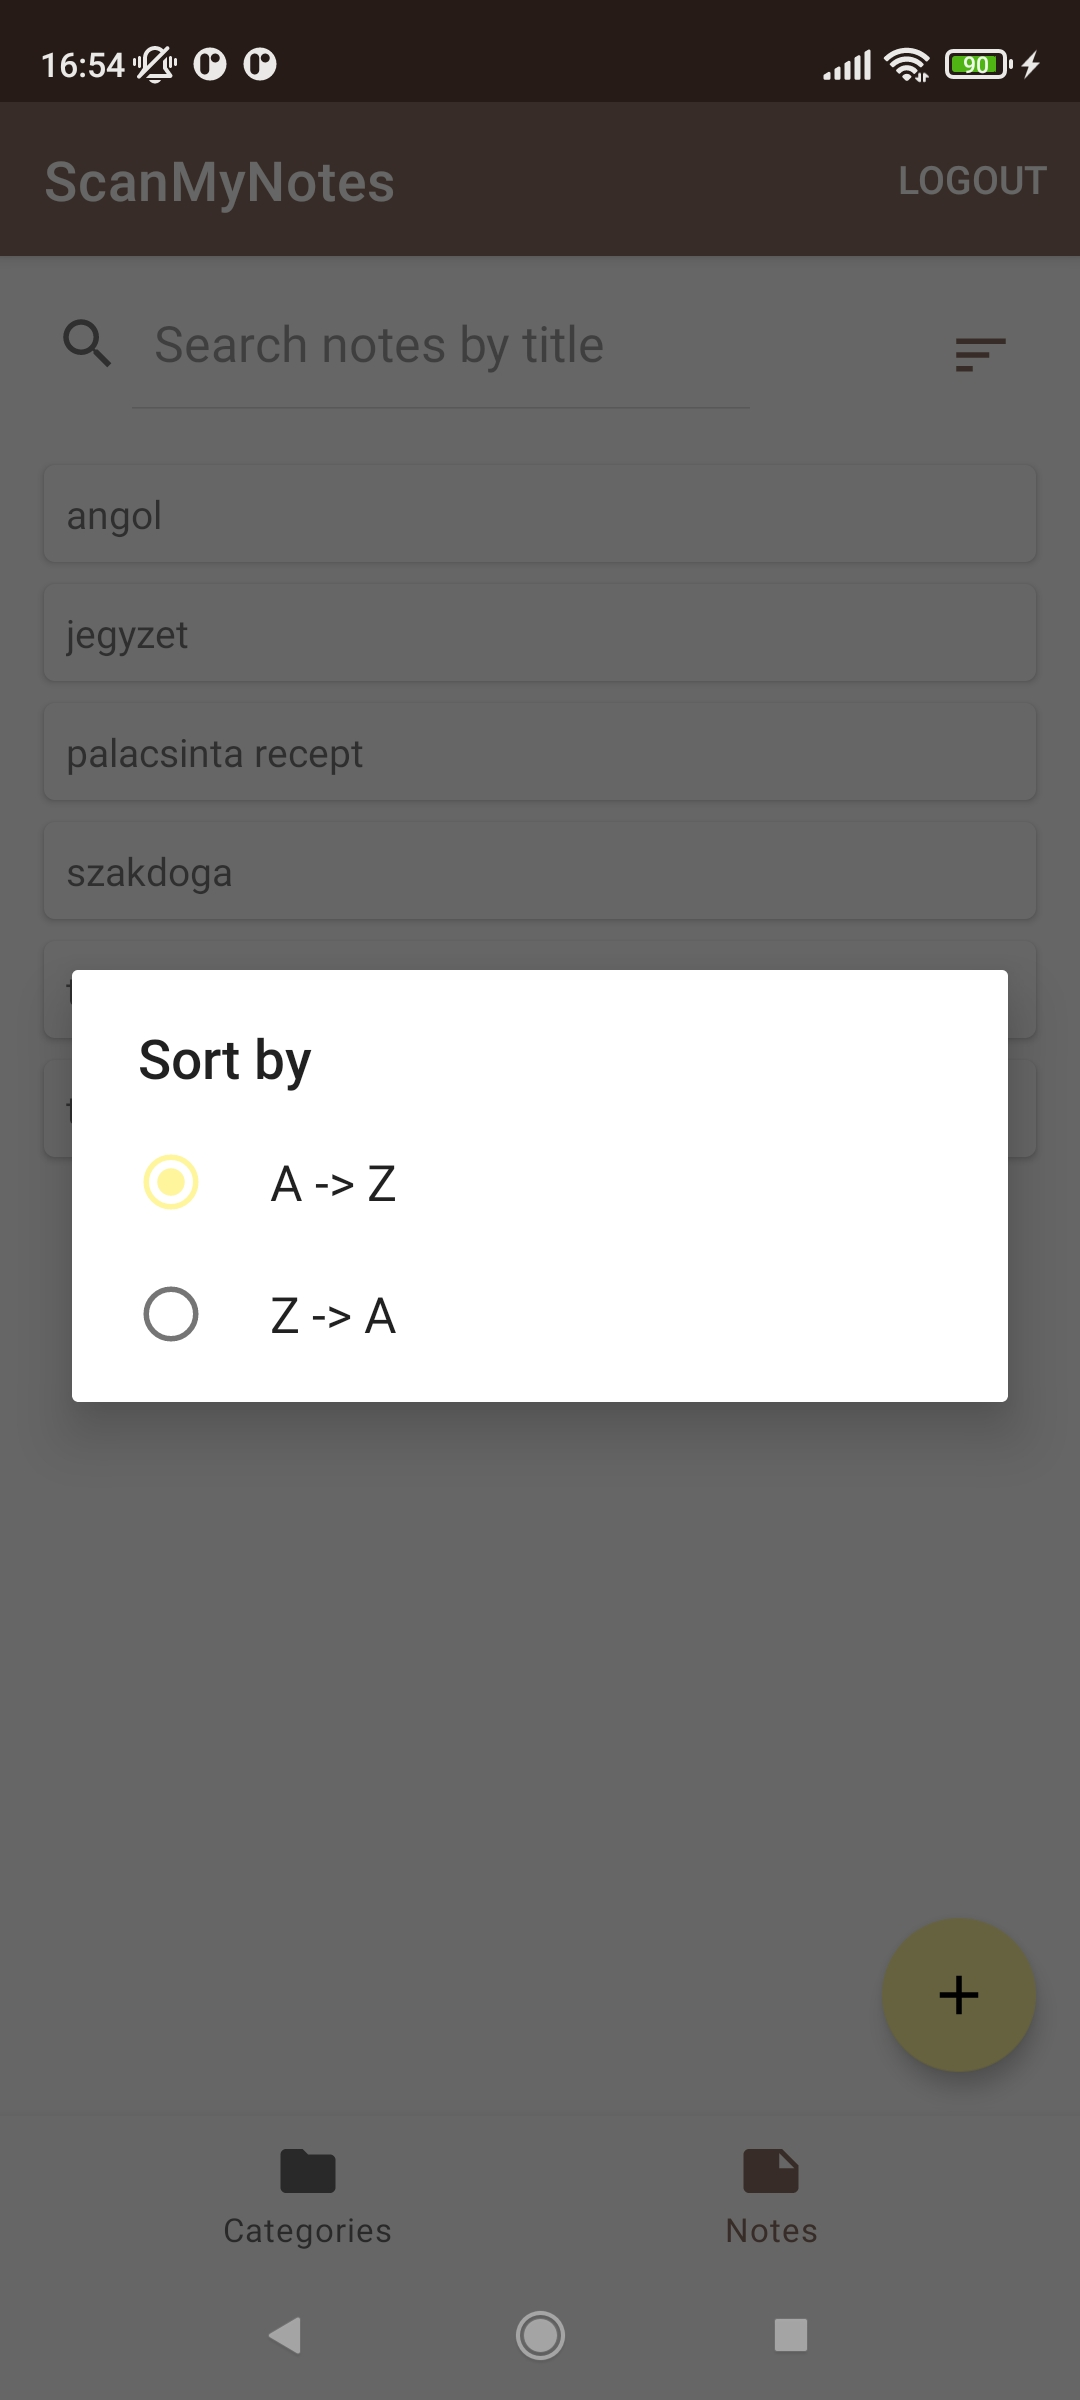
\includegraphics[width=49mm, keepaspectratio]{figures/notelist_sort.jpg}
	\caption{A jegyzetek listája, és a rajta elvégezhető műveletek.}
	\label{fig:NoteListScreen2}
\end{figure}

\subsection{Jegyzet létrehozása}
Az alkalmazás fő funkcionalitása a jegyzetek tárolása, így elég fontos, hogy legyen lehetőség újak létrehozására. Ez a képernyő jobb alsó sarkában található plusz gombra kattintva tehető meg. Az ott megjelenő két újabb gomb közül az alsó megnyomására felugrik egy kameraablak, ahol egy fénykép készítése után megtörténik a digitalizáció, és a szerkesztési oldalra ugrunk. Itt egy cím megadásával fejezhetjük be a létrehozási folyamatot, de opcionálisan hozzárendelhetjük egy kategóriához is (\refstruc{fig:NewNoteScreen}). Amíg a cím vagy a tartalom üres, addig az alkalmazás nem fogja engedni elmenteni a jegyzetet, figyelmeztetést rak az üresen hagyott mezőre.
\begin{figure}[!ht]
	\centering
	
\includegraphics[width=55mm, keepaspectratio]{figures/newnote_photo.jpg}
	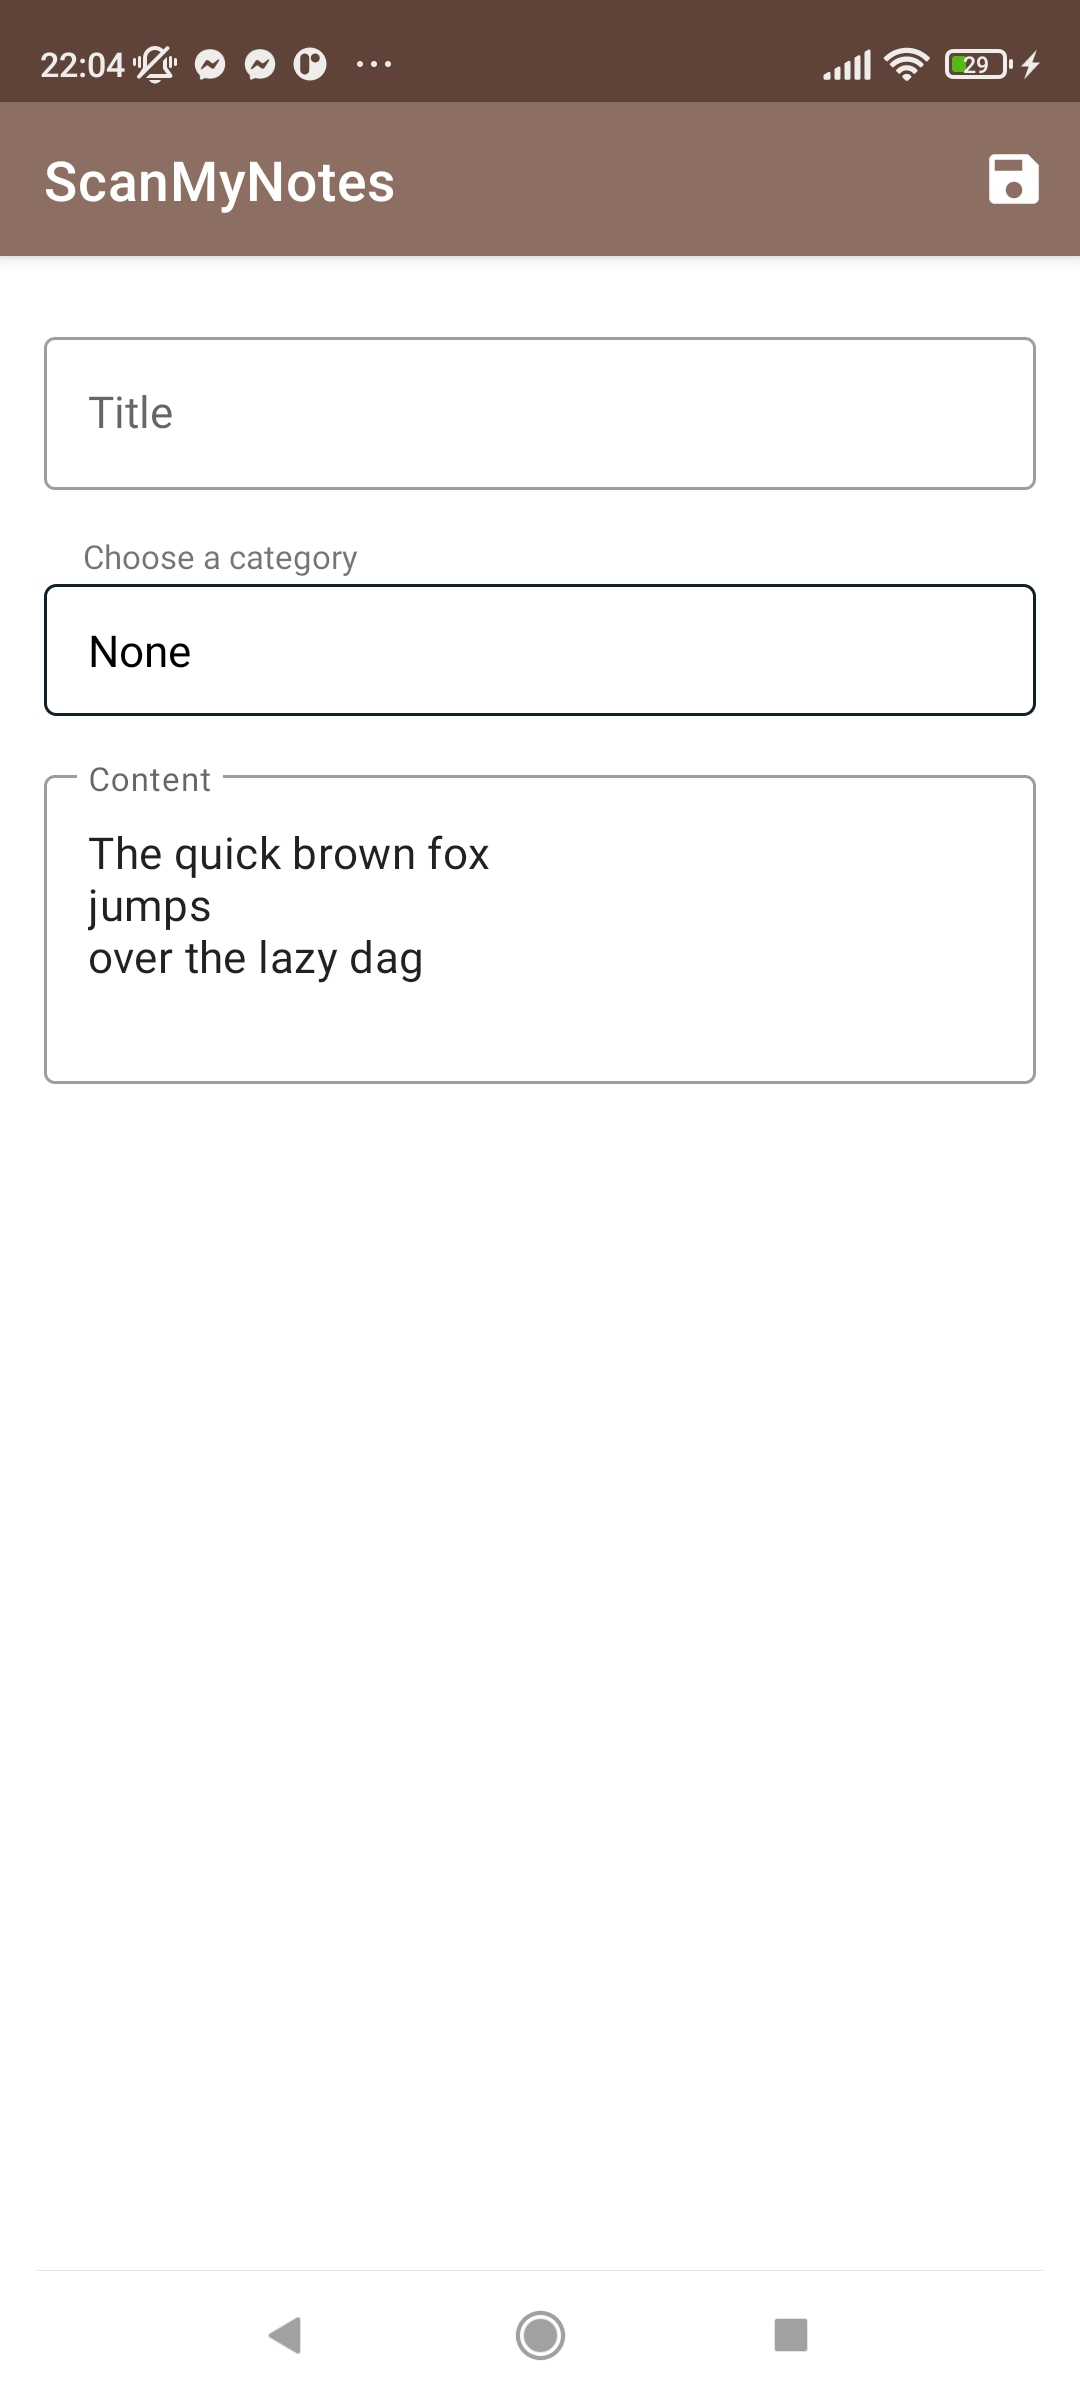
\includegraphics[width=55mm, keepaspectratio]{figures/newnote_create.jpg}
	\caption{A létrehozás során készített kép, illetve az abból kialakuló jegyzet szerkesztése.}
	\label{fig:NewNoteScreen}
\end{figure}

\subsection{Jegyzet szerkesztése}
Amennyiben a listában egy jegyzetre kattintunk, illetve újat hozunk létre, akkor annak részletes oldalára navigálunk. Itt megtekinthetjük a tartalmát, a jobb felső sarokban található ceruza ikonra nyomva pedig szerkeszthetjük is (\refstruc{fig:NoteDetailsScreen}). Megváltoztathatjuk a címét, tartalmát, kategóriáját, a fent megjelenő pluszjel segítségével pedig készíthetünk újabb fotót, melynek szövege hozzáfűzésre kerül az eddigihez. A fentebb említett megkötések itt is érvényesek, azaz a cím és a tartalom nem lehet üres az elmentés pillanatában. 

Mind megtekintési, mind szerkesztési módban elérhető a fenti sávban a szemetes ikon, mellyel törölhetjük a jegyzetet a listánkból. Vigyázat, ez a művelet nem visszafordítható! 

\begin{figure}[!ht]
	\centering
	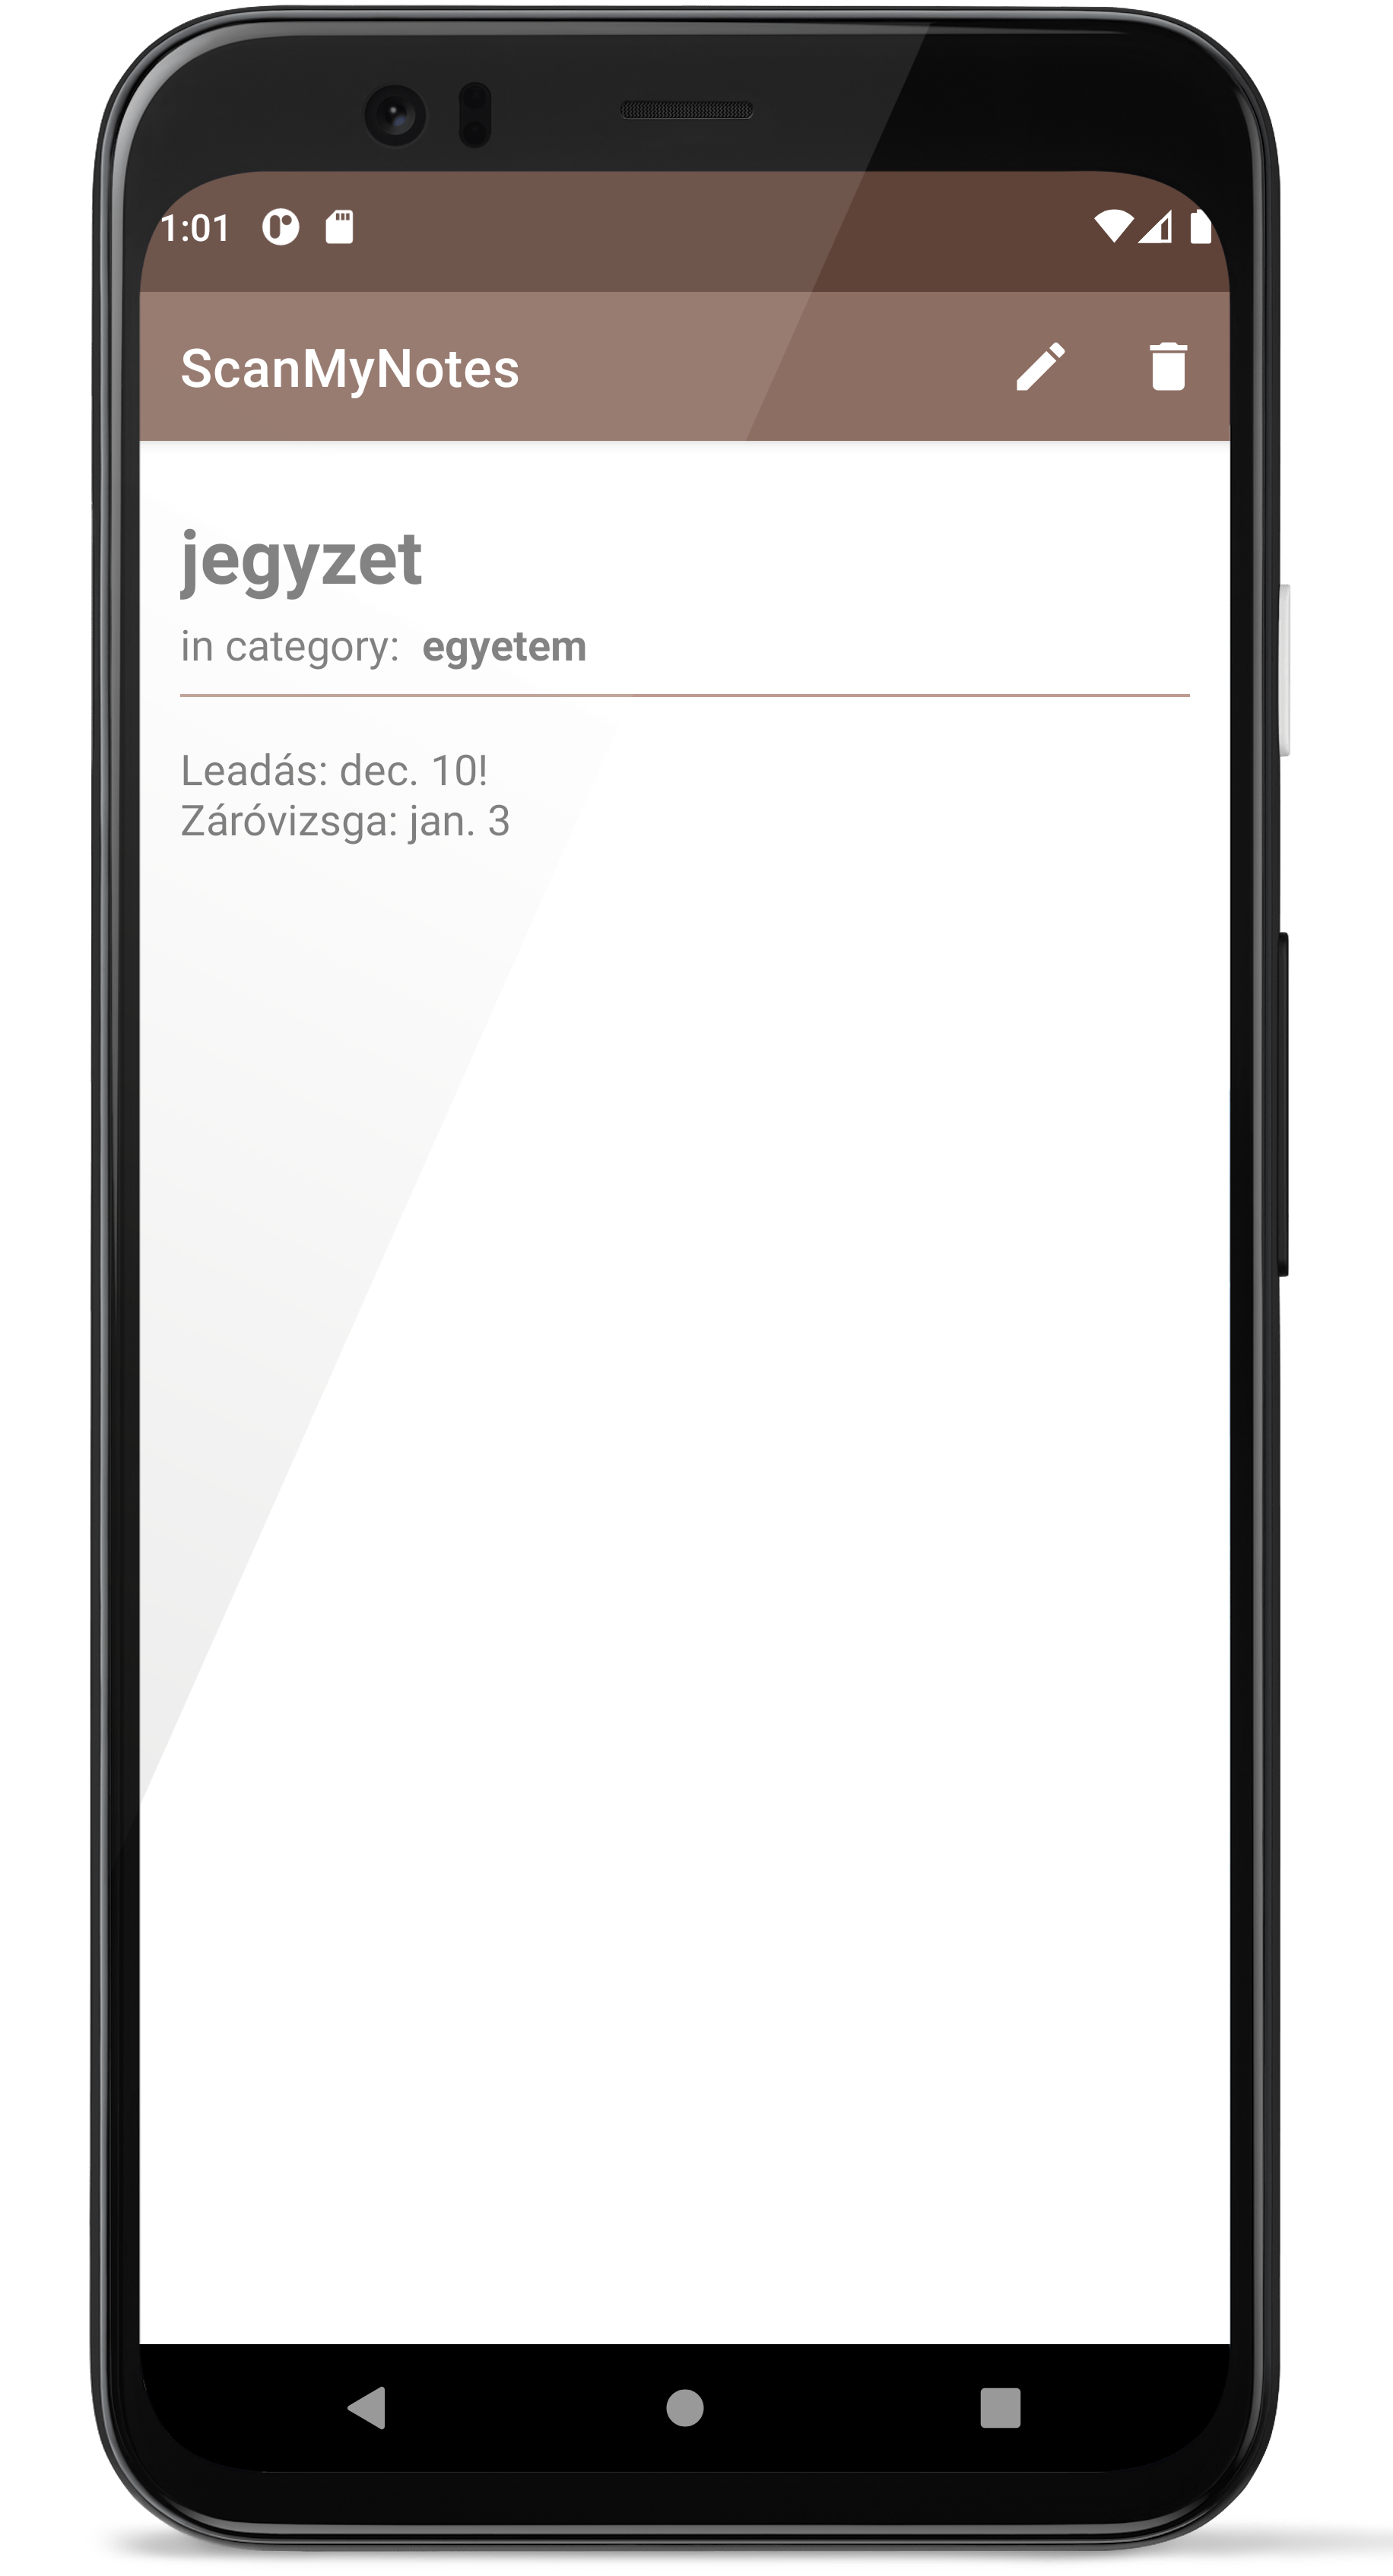
\includegraphics[width=55mm, keepaspectratio]{figures/note_view.png}
	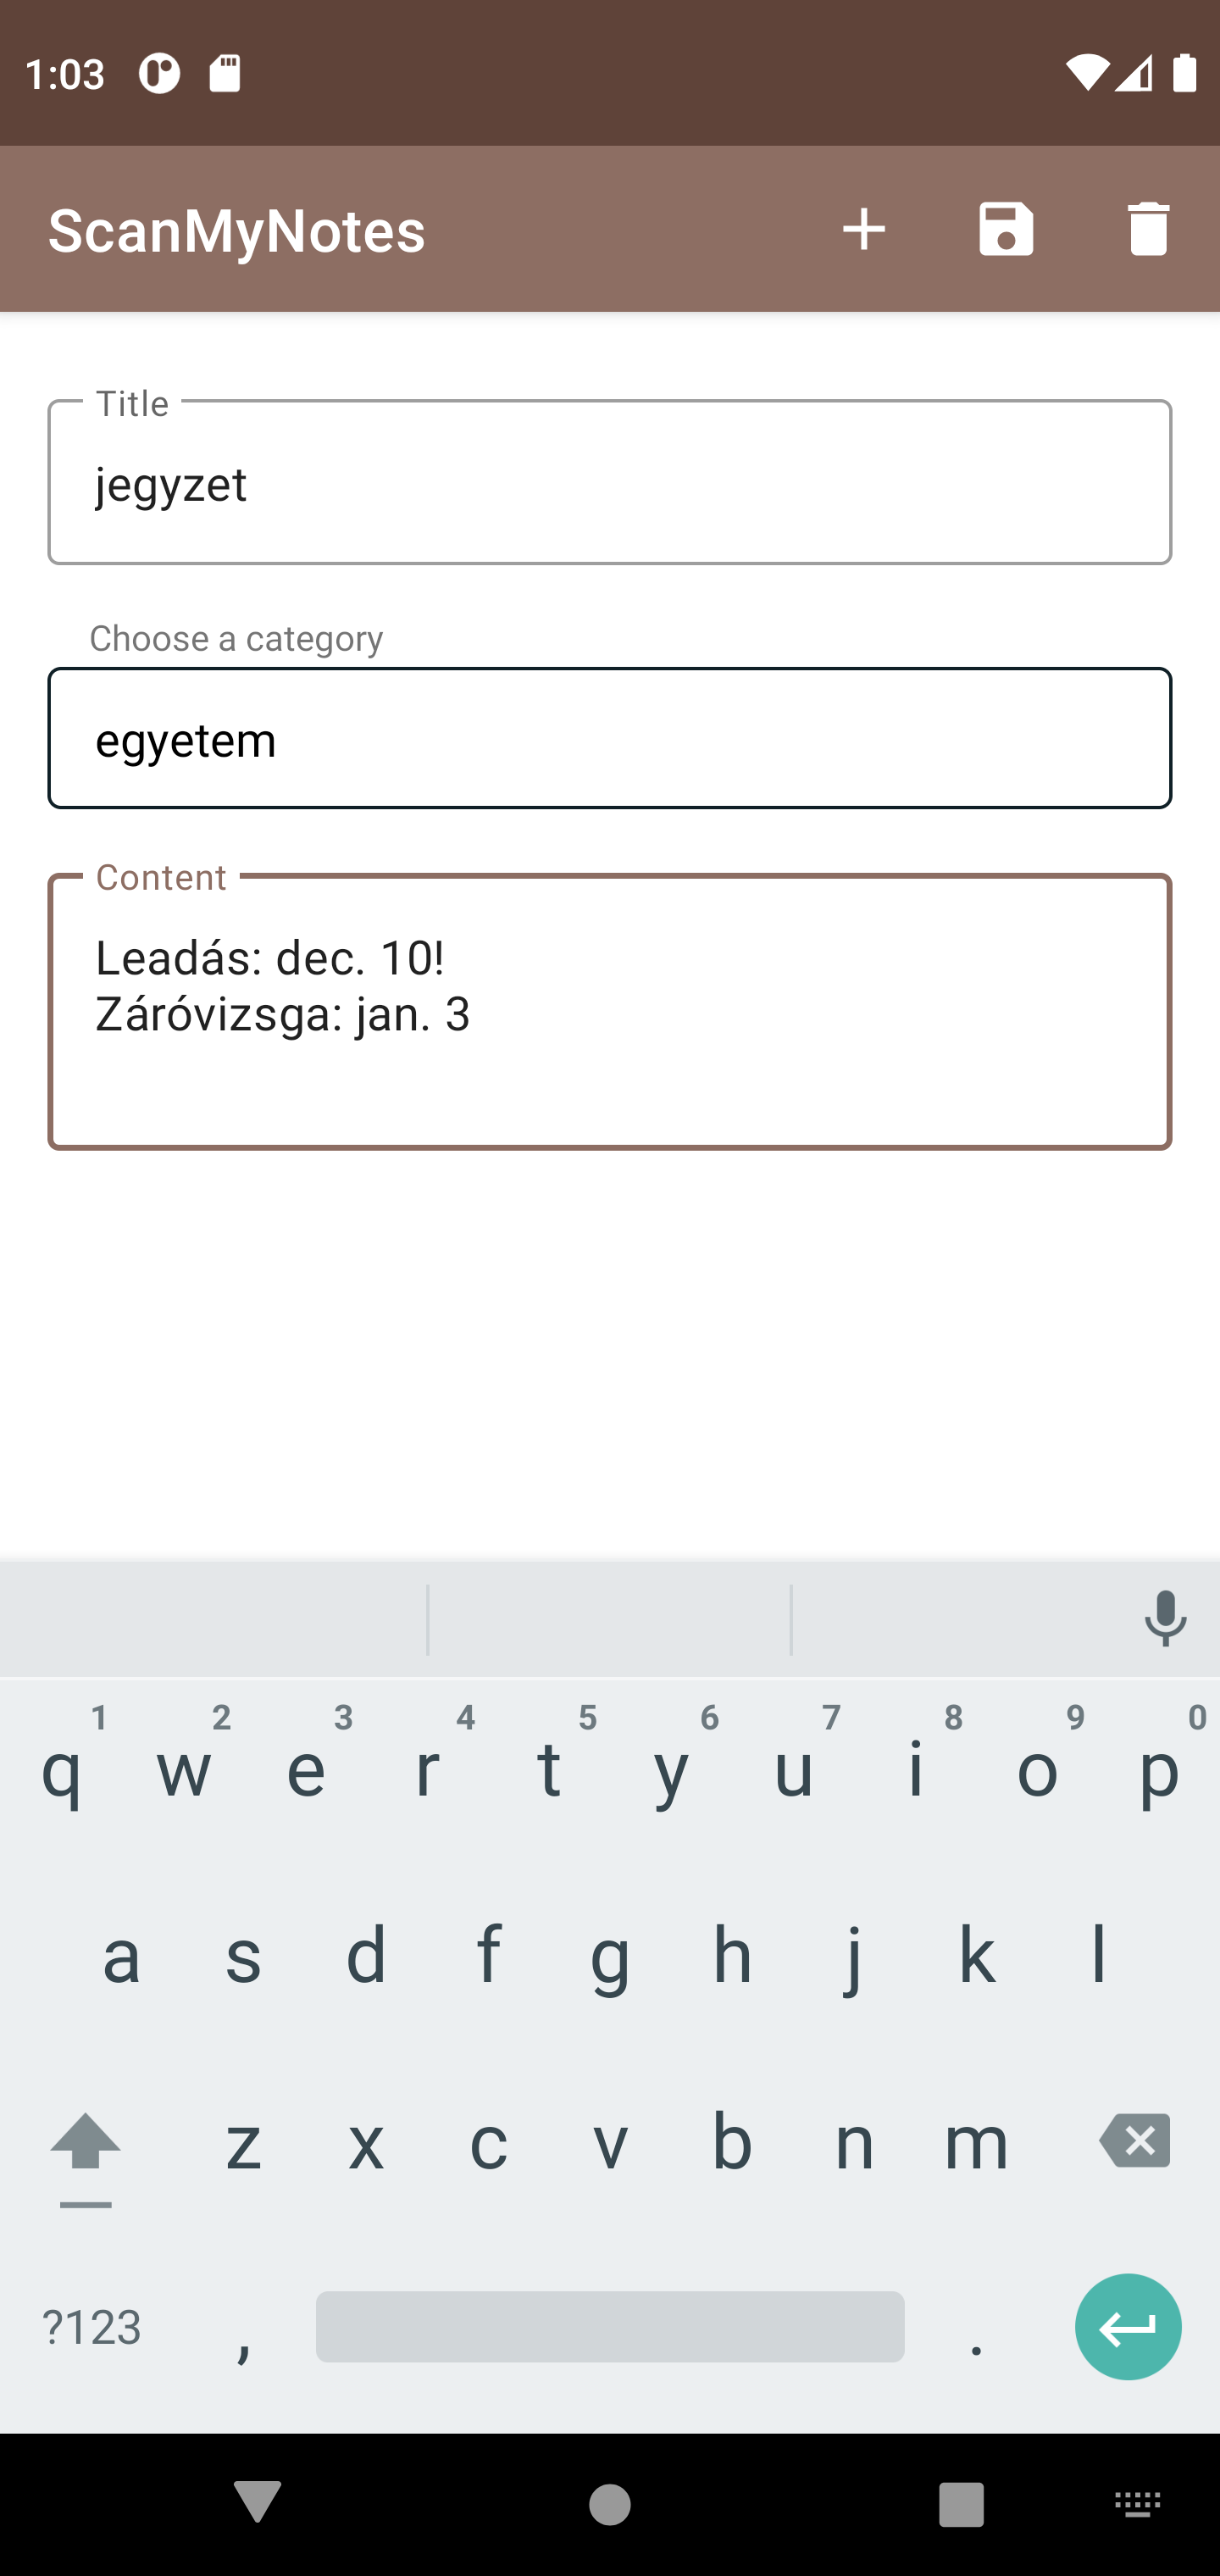
\includegraphics[width=55mm, keepaspectratio]{figures/note_edit.png}
	\caption{A jegyzet megtekintési, illetve szerkesztési képernyője.}
	\label{fig:NoteDetailsScreen}
\end{figure}

\subsection{Kategória létrehozása}
Az alkalmazásban elérhető másik adattípus a kategória, mely rendszerezési célt szolgál. Képes magába foglalni jegyzeteket és más kategóriákat is, tetszőleges mélységben. Szintén a jobb alsó sarokban található gomb biztosítja a létrehozás lehetőségét, ám ebben az esetben a felugró két kisebb gomb közül a felsőt kell választani. Itt egy, a jegyzetkészítéshez nagyon hasonló oldalon tudunk címet és opcionálisan szülőkategóriát megadni, és amennyiben nem üres a cím mezője, el is menthetjük (\refstruc{fig:NewCategoryScreen}). 

\begin{figure}[!ht]
	\centering
	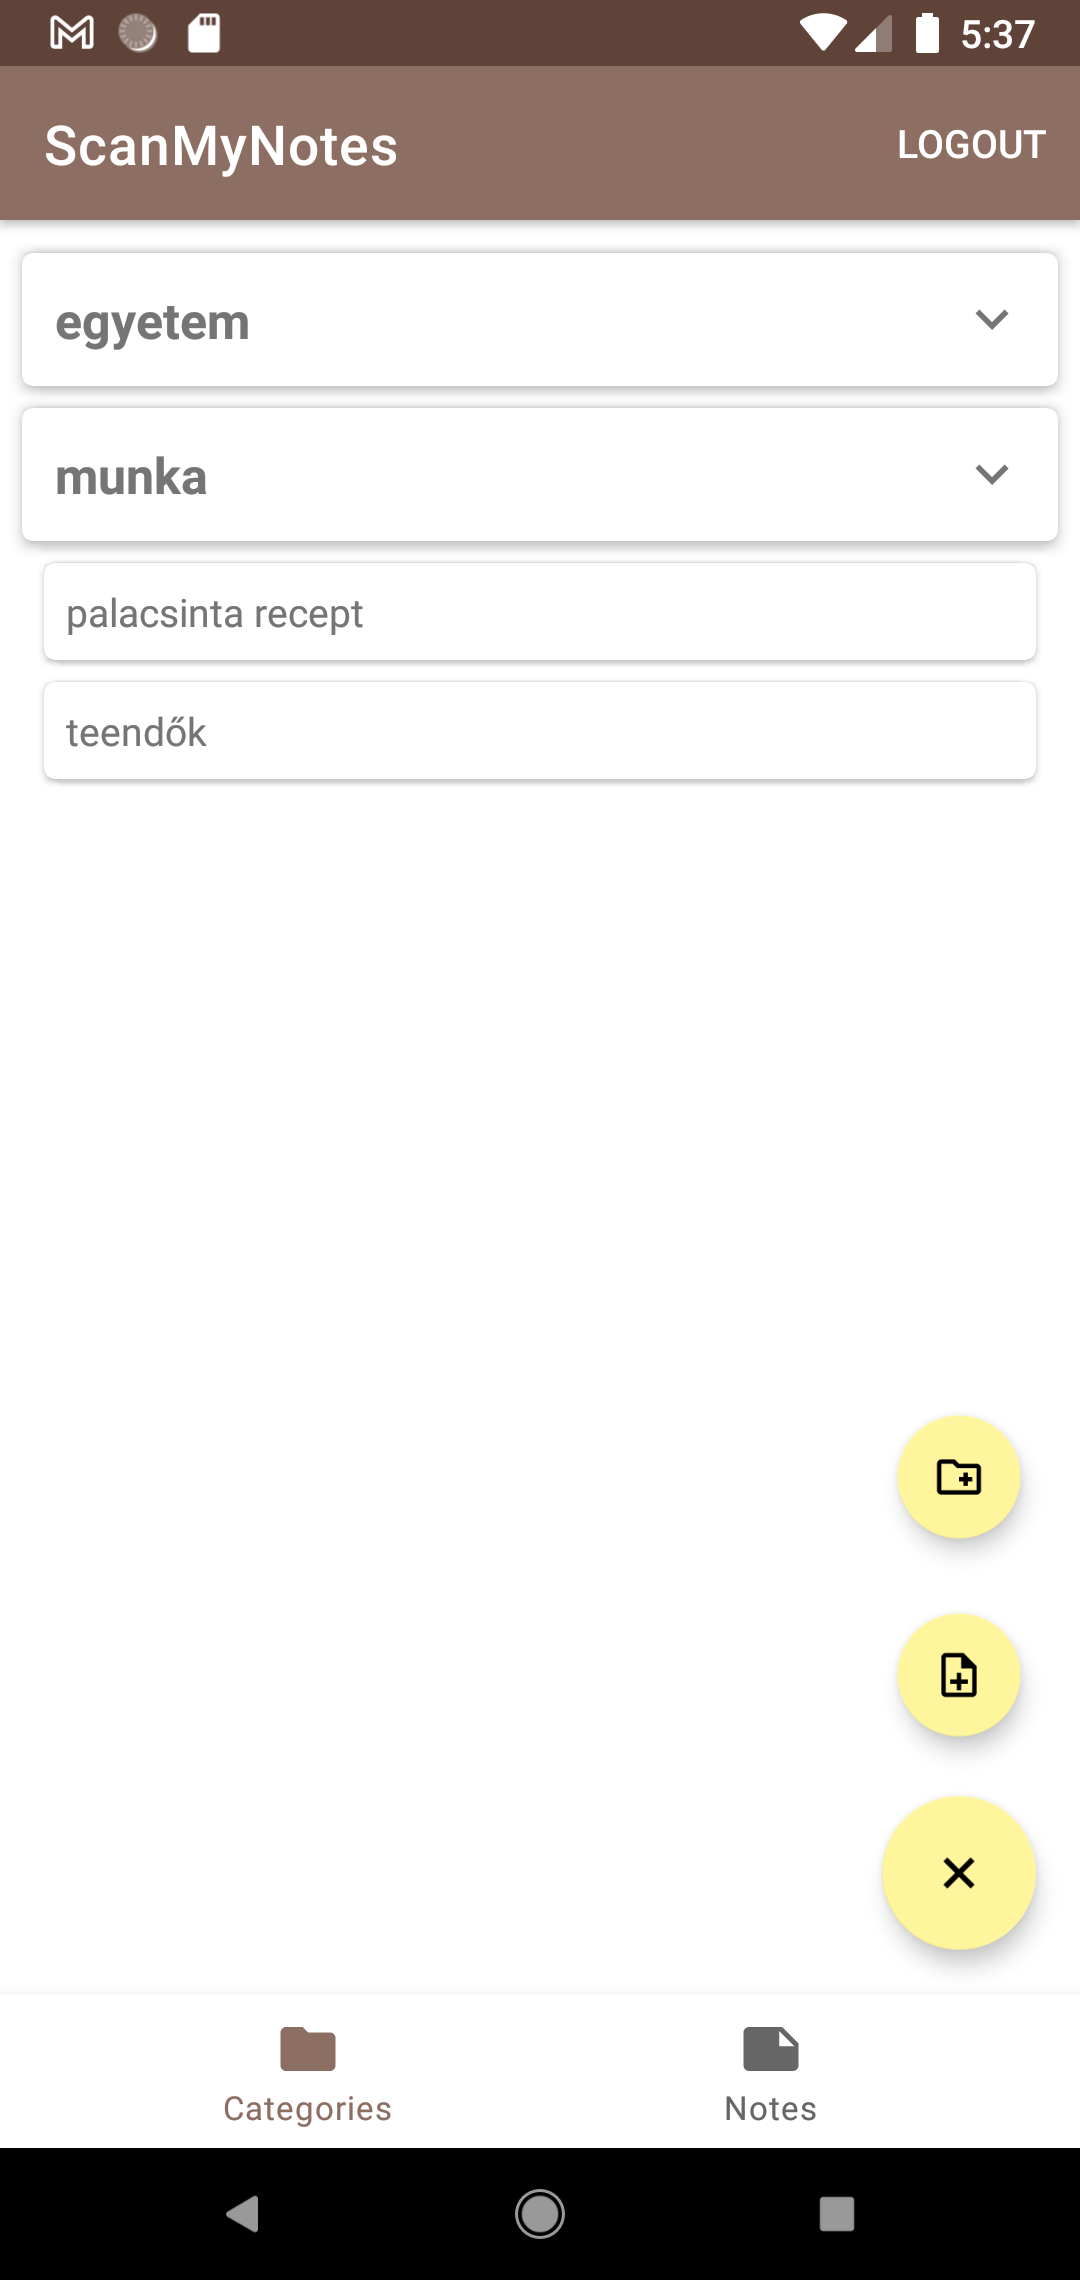
\includegraphics[width=50mm, keepaspectratio]{figures/floatingbutton_open.png}
	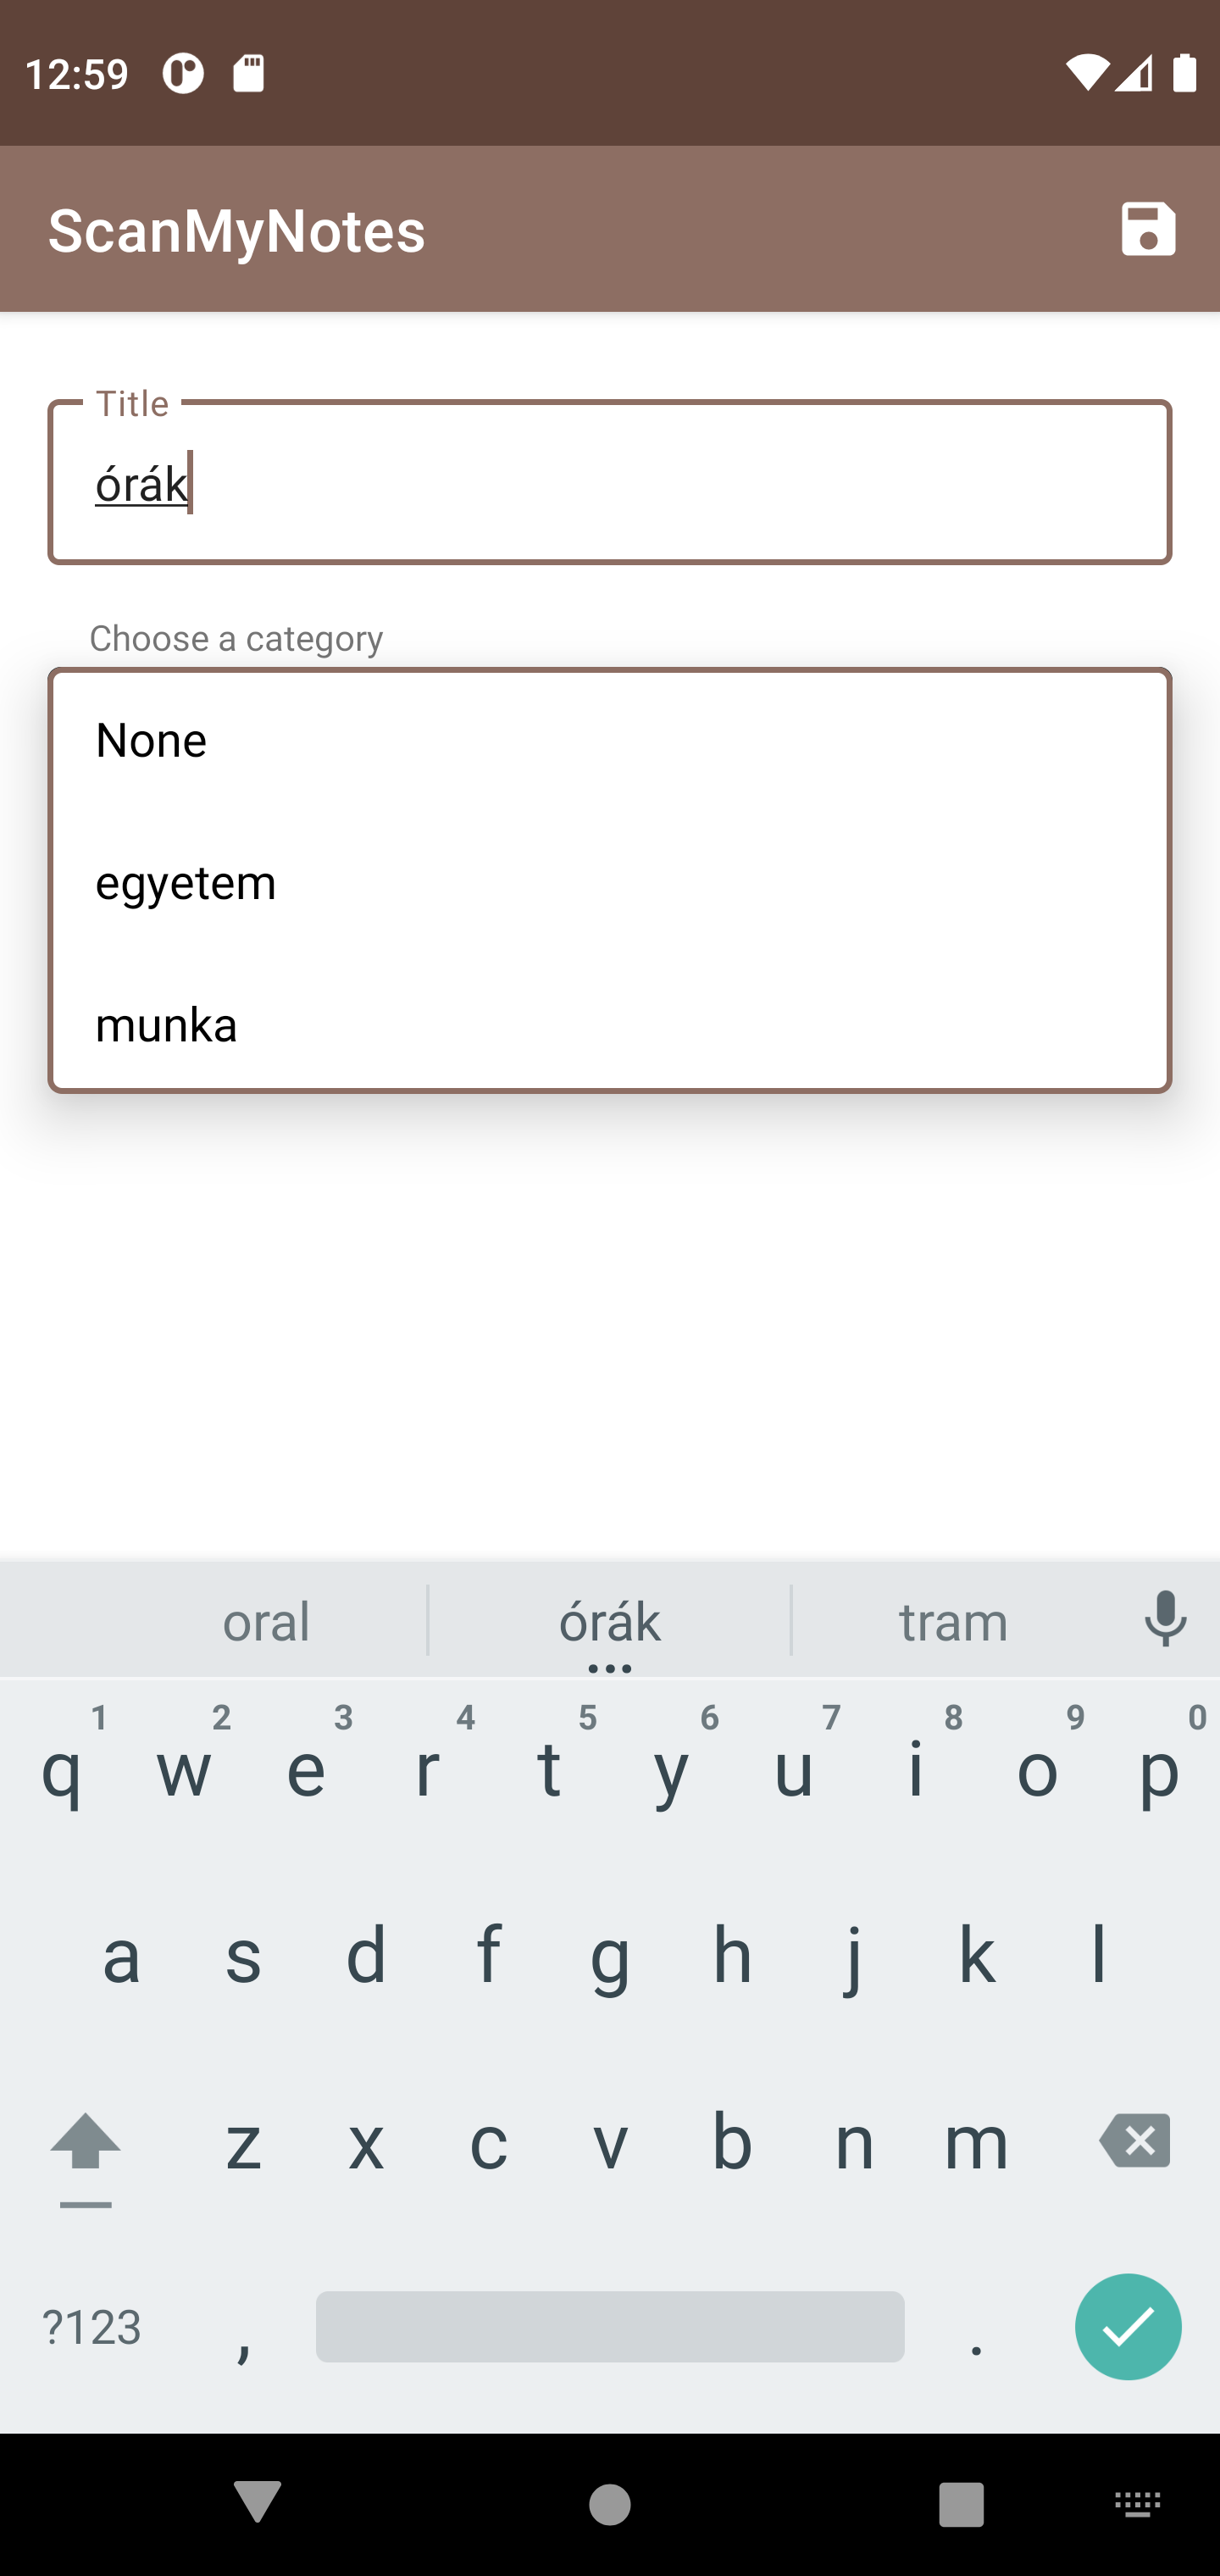
\includegraphics[width=50mm, keepaspectratio]{figures/category_save.png}
	\caption{A létrehozás gomb kinyitott állapotban, új kategória felvétele.}
	\label{fig:NewCategoryScreen}
\end{figure}

\subsection{Kategória szerkesztése}
Új kategória létrehozása után, illetve a listában egy kategóriára nyomva annak részleteit tekinthetjük meg. Itt megjelenik a címe és esetleges szülője, és jobb fent szintén található egy ceruza ikon, mely lehetővé teszi a szerkesztést (\refstruc{fig:CategoryDetailsScreen}). Hasonlóan a jegyzethez megtekintés és szerkesztés során is törölhetjük az adott kategóriát, ilyenkor egy felugró ablak figyelmeztet rá, hogy a törlés során az összes tartalmazott objektum is törlődni fog. 

\begin{figure}[!ht]
	\centering
	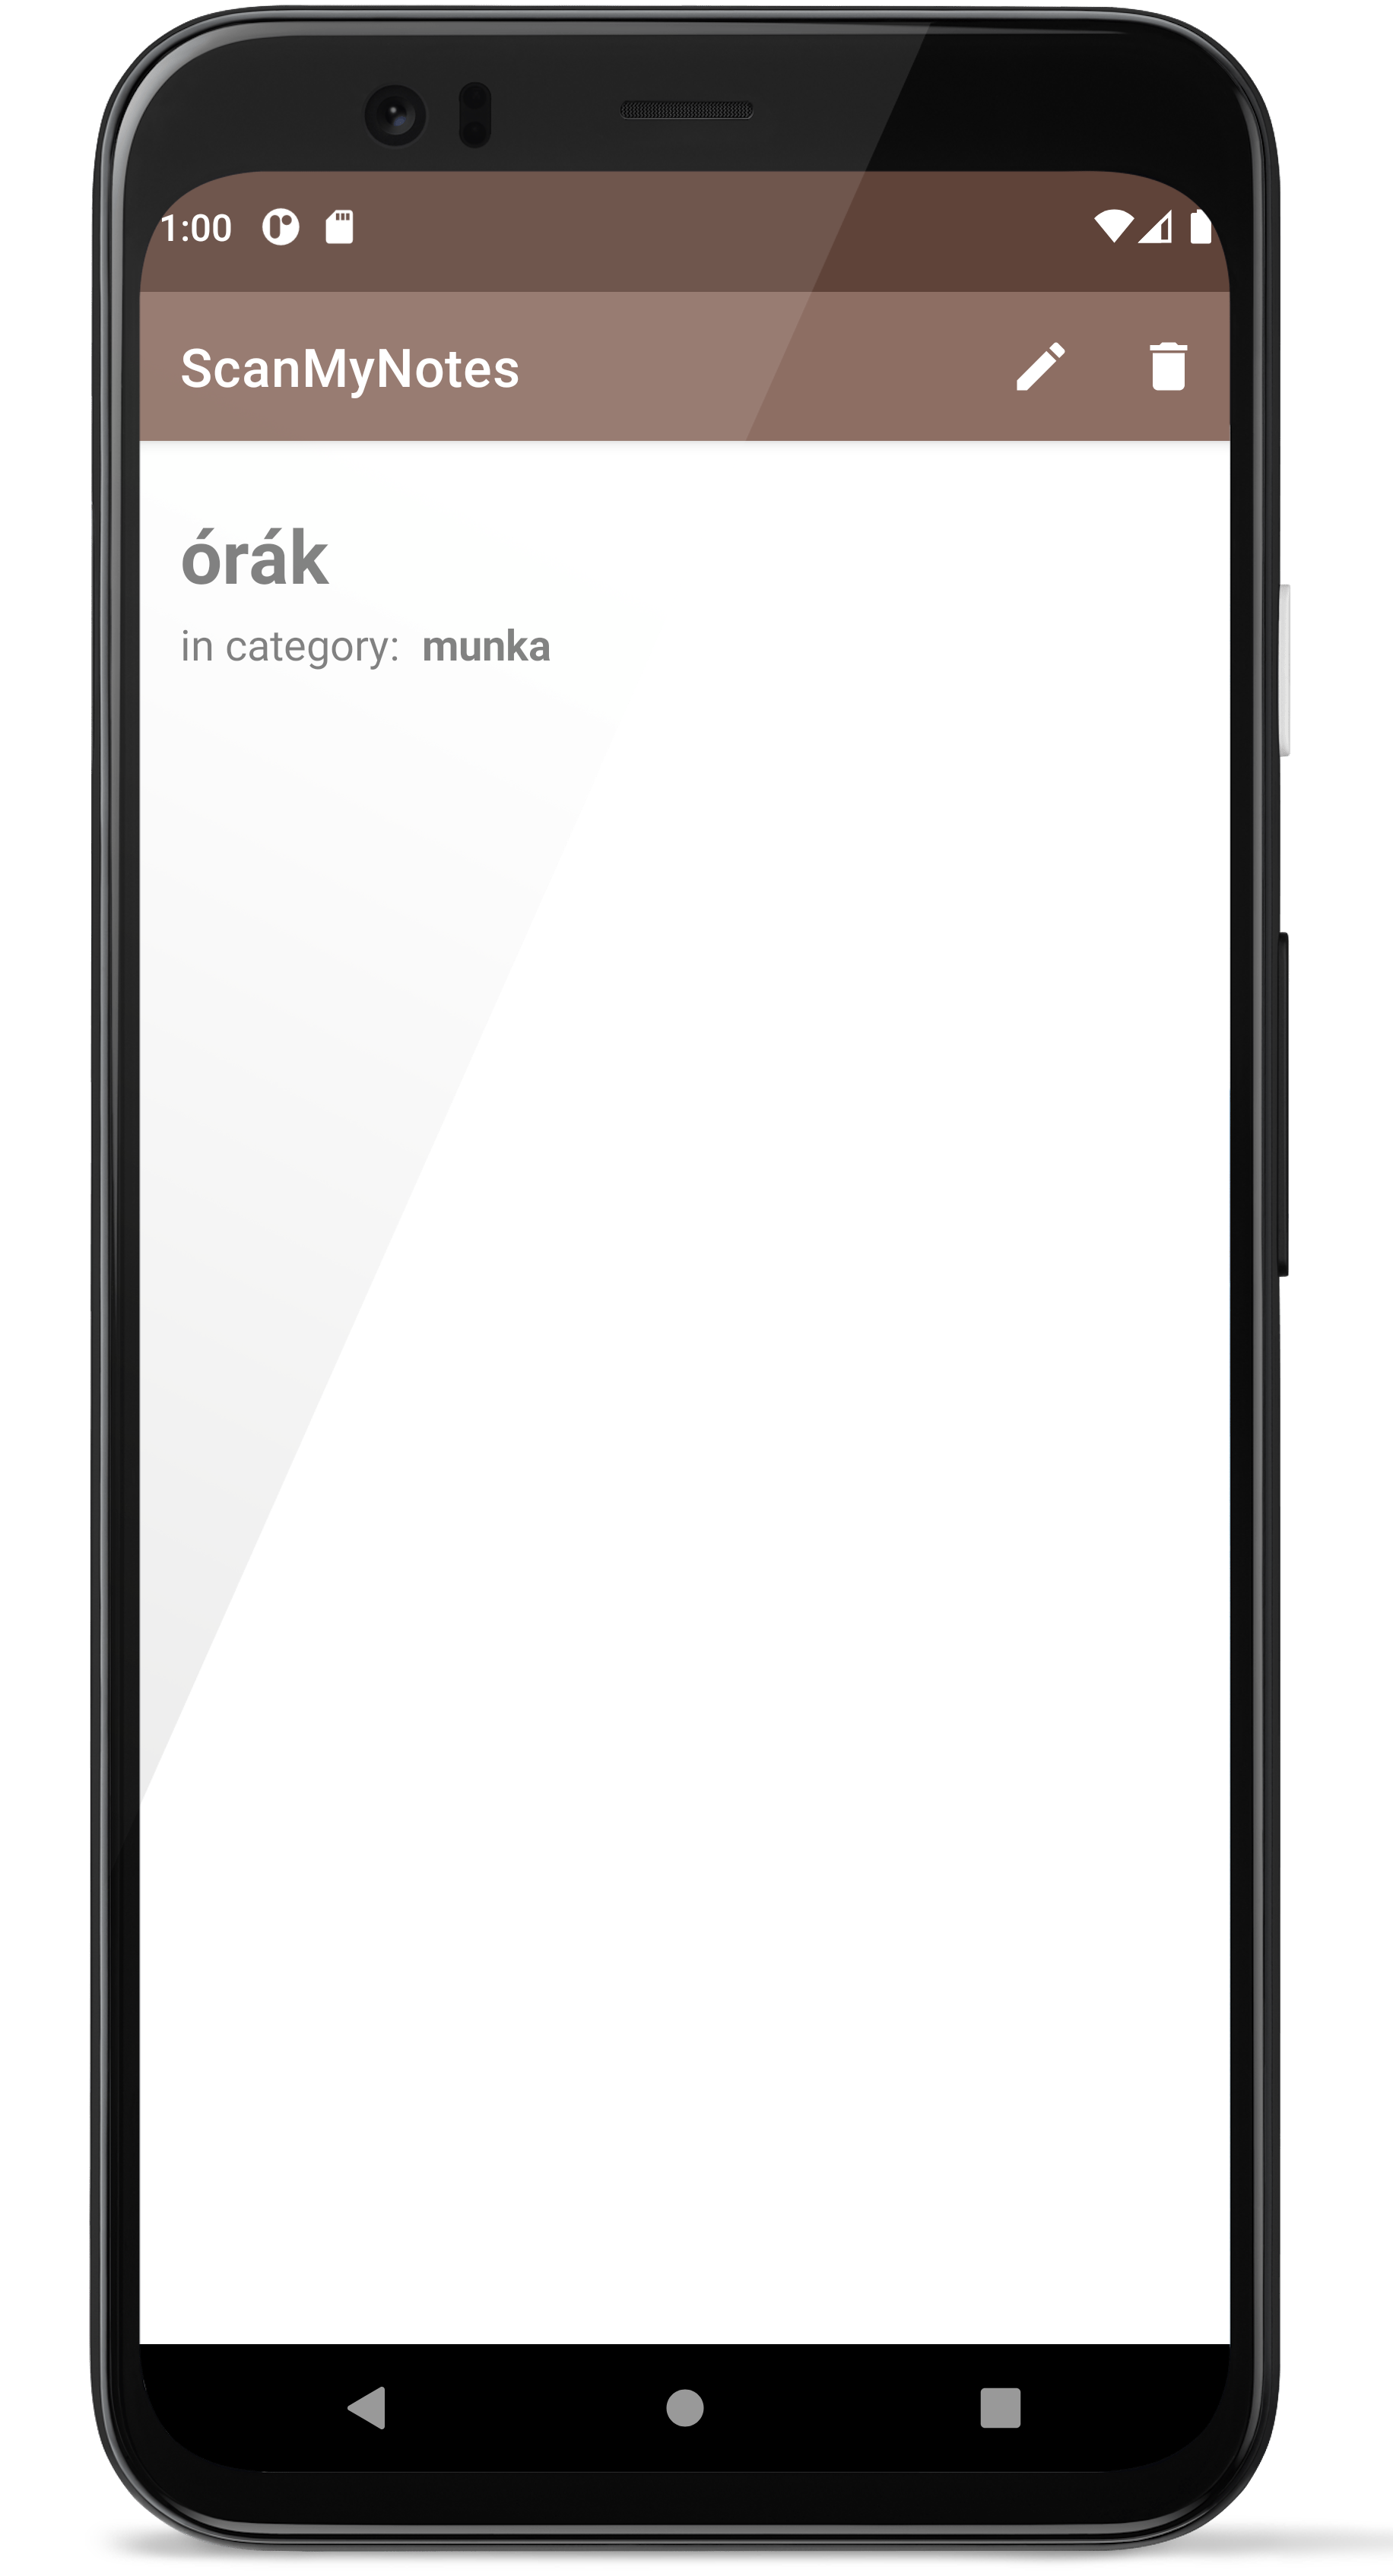
\includegraphics[width=50mm, keepaspectratio]{figures/category_view.png}
	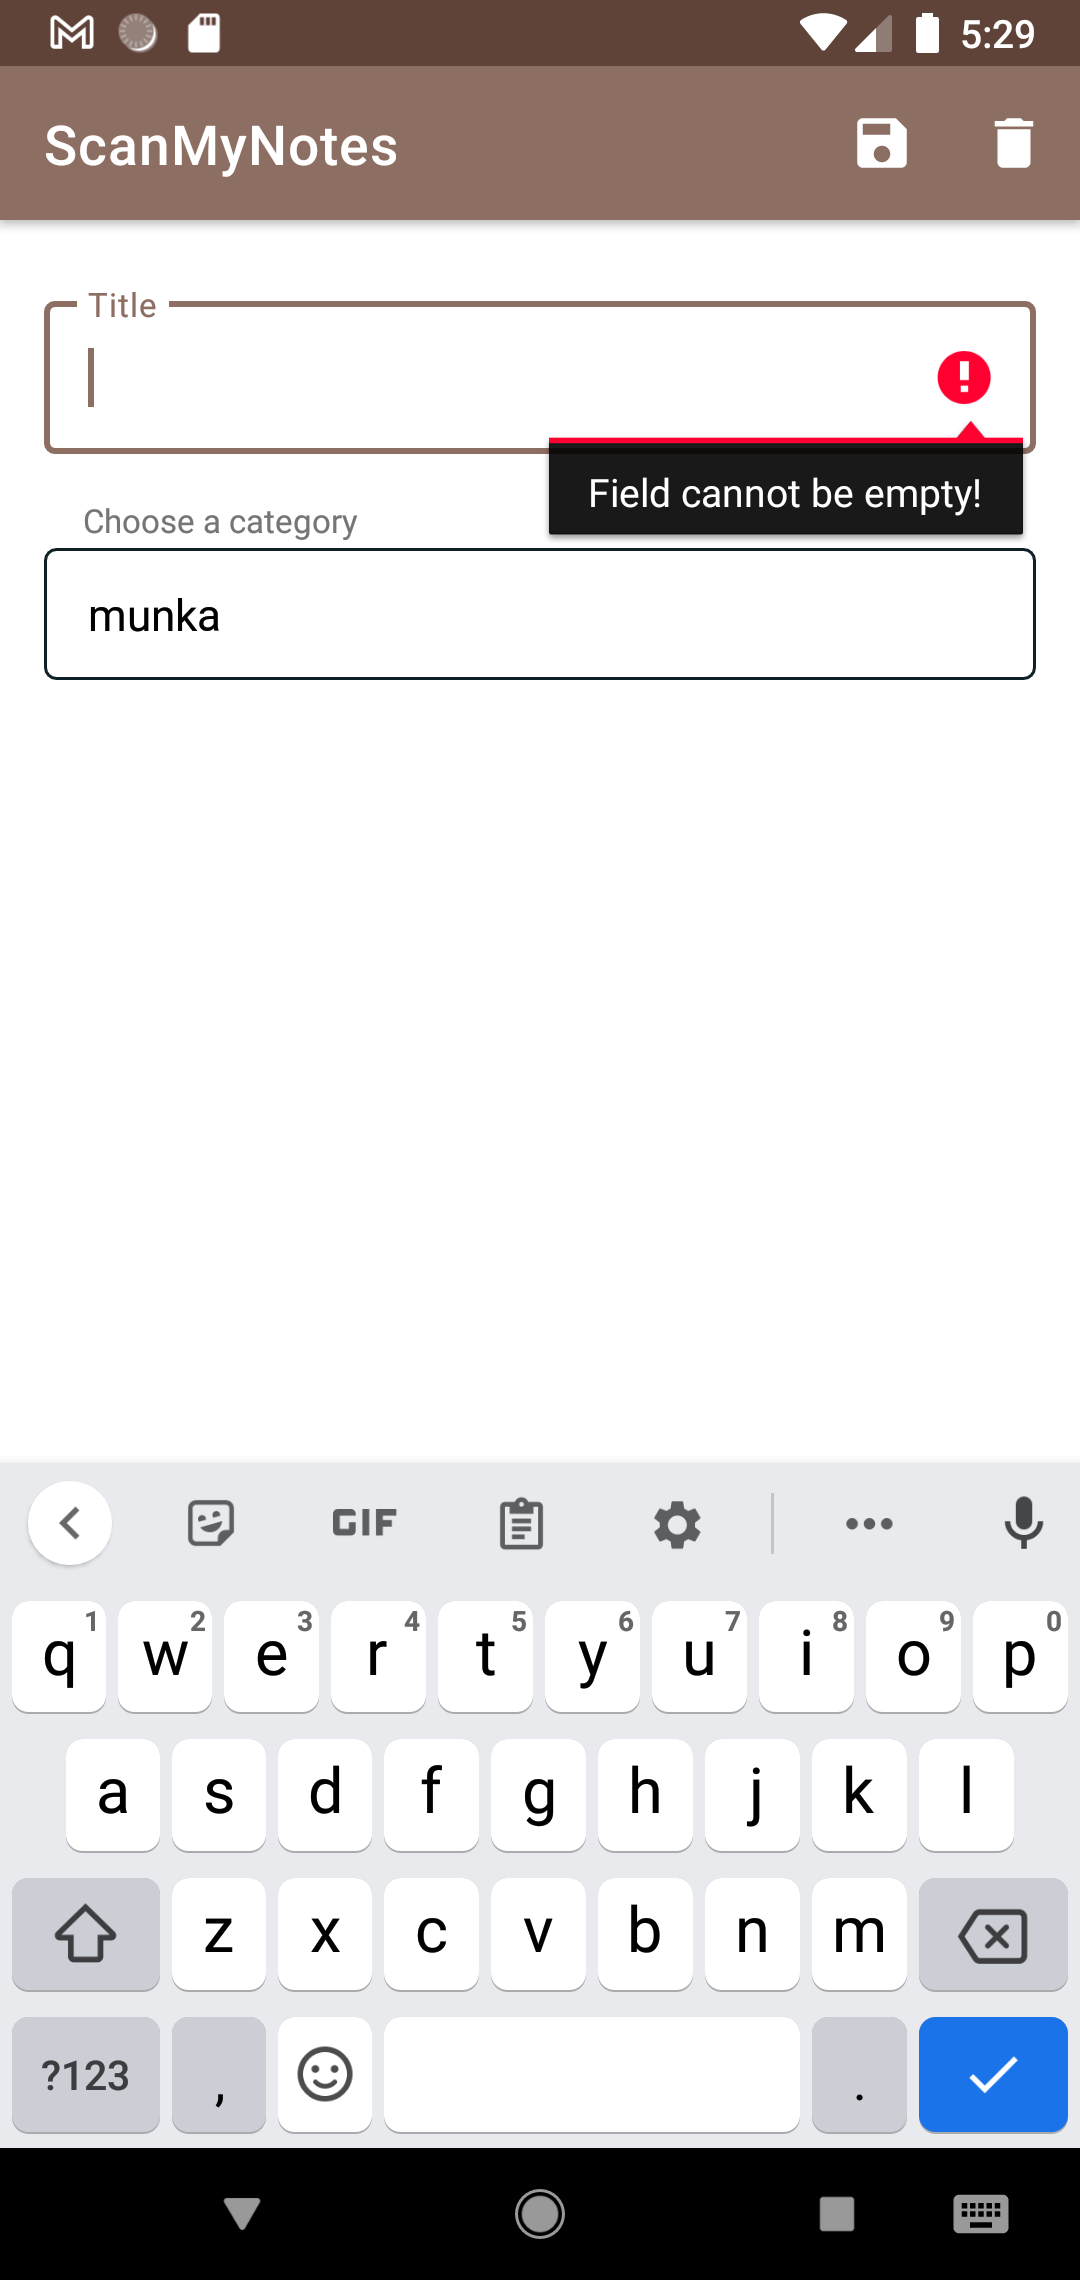
\includegraphics[width=50mm, keepaspectratio]{figures/category_edit_error.png}
	\caption{A kategória részletes képernyője, illetve a szerkesztési képernyő által feldobott hiba, ha üresen hagyjuk a címet.}
	\label{fig:CategoryDetailsScreen}
\end{figure}

\section{Tesztelés}
%--------------------
\chapter{Összefoglalás}
%--------------------

%TODO

\section{Tapasztalatok}

\section{Értékelés}

Az 5. fejezetben az alkalmazás követelményei résznél 10 pontba szedtem az applikációval szemben támasztott elvárásokat, így most arra szeretnék kitérni pontonként, hogy ezeket mennyire sikerült megvalósítani.

\begin{enumerate}
	\item A felhasználói fiók létrehozására és a bejelentkezésre létrejött egy képernyő, ahol egy e-mail címet és egy jelszót kell megadni. Magát az autentikációt a Firebase Authentication végzi. Belépés után a NoteList képernyő jobb felső sarkában található Logout gomb nyújt lehetőséget a kijelentkezésre.
	\item Az adatok tárolásáért a Firebase Firestore a felelős, és mivel ez egy felhőalapú szolgáltatás, így az bárhonnan, bármikor elérhető bejelentkezést követően. Nem kell tehát a felhasználónak azzal foglalkoznia, hogy biztonsági másolatot készítsen a jegyzeteiről arra az esetre, ha elromlana/eltűnne a telefonja, csupán annyit kell tennie, hogy egy másik készülékre letölti az applikációt és bejelentkezik.
	\item A bejelentkezési oldalról addig nem lehet tovább navigálni, amíg nem lett sikeres az autentikáció. A saját adatok elérése pedig az adattárolás struktúrájából következik, ugyanis az adatbázisban minden felhasználó adata a saját azonosítójával elnevezett dokumentumban található, futás során pedig az auth modul csak a jelenleg bejelentkezett felhasználó id-ját ismeri, és ezt használja fel a megfelelő dokumentum lekéréséhez. 
	\item A kategóriákkal szemben támasztott követelményeket sikerült maradéktalanul teljesíteni, van egy új kategória nézet, ahol nevet és szülőt lehet adni a kategóriának. A Category modell pedig biztosítja a tetszőleges mélységű egymásba ágyazást, ugyanis a \emph{listItems} adattagja további kategóriákat is tartalmazhat, melyek szintén tartalmazhatnak kategóriákat és így tovább. 
	\item Egy fénykép készítése után - amennyiben volt rajta felismerhető szöveg - annak tartalmából jegyzet készíthető, a megjelenő létrehozás képernyőn címet adhatunk és kategóriát választhatunk neki, és a detektált szöveg is szerkeszthető mentés előtt. 
	\item 
	\item
	\item
	\item
	\item
\end{enumerate}

Mindezt figyelembe véve én elégedett vagyok az elkészült alkalmazással, mert bár még elég alap funkcionalitással rendelkezik, de úgy gondolom, hogy a lehető legjobban figyeltem arra, hogy könnyen bővíthetővé tegyem. Van is nem kevés ötletem a potenciális fejlesztésekre, melyből néhányat a következő szekcióban ismertetek. 

\section{Továbbfejlesztési lehetőségek}

Egy alkalmazás fejlesztése soha nem ér véget abból a szempontból, hogy mindig lehet szebbé és jobbá alakítani. A félév végére egy egész komplex projekt alakult ki, de lezárásképp még megemlítek pár dolgot, amiben tovább lehetne fejleszteni.
%%----------------------------------------------------------------------------
\chapter{\LaTeX-eszközök}
\label{sec:LatexTools}
%----------------------------------------------------------------------------
\section{A szerkesztéshez használatos eszközök}
%----------------------------------------------------------------------------
Ez a sablon TeXstudio 2.8.8 szerkesztővel készült. A TeXstudio egy platformfüggetlen, Windows, Linux és Mac OS alatt is elérhető \LaTeX-szerkesztőprogram számtalan hasznos szolgáltatással (\refstruc{fig:TeXstudio}). A szoftver ingyenesen letölthető\footnote{A TeXstudio hivatalos oldala: \url{http://texstudio.sourceforge.net/}}.

\begin{figure}[!ht]
\centering
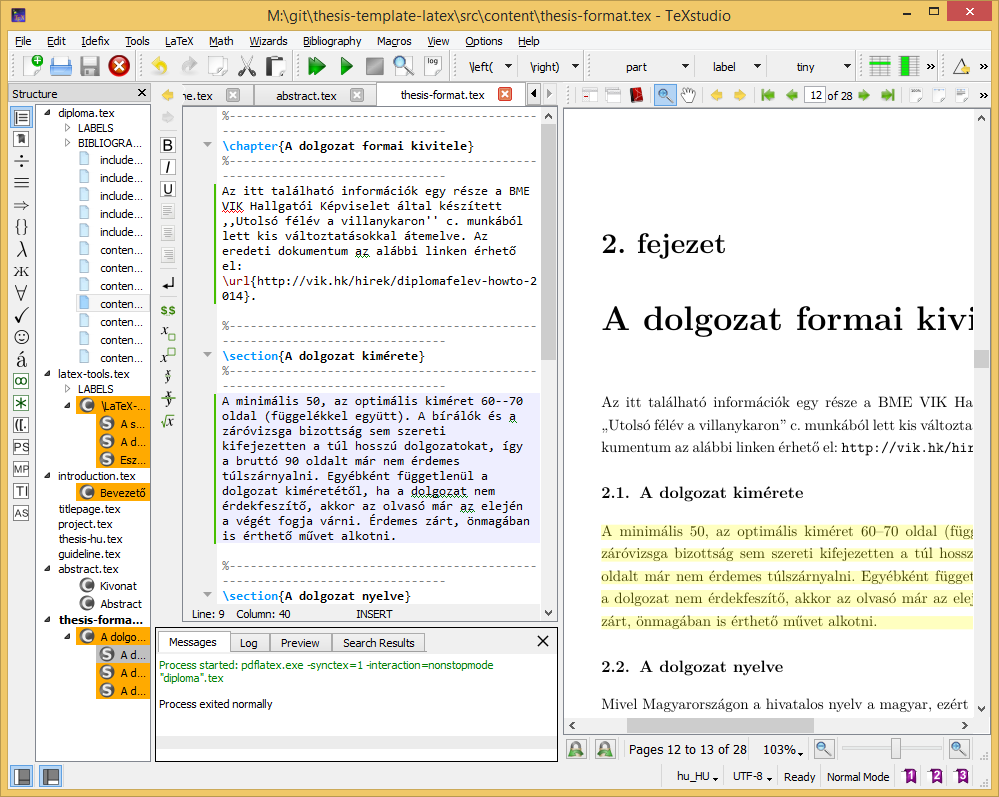
\includegraphics[width=150mm, keepaspectratio]{figures/TeXstudio.png}
\caption{A TeXstudio \LaTeX-szerkesztő.}
\label{fig:TeXstudio}
\end{figure}

A TeXstudio telepítése után érdemes még letölteni a magyar nyelvű helyesírásellenőrző-szótárakat hozzá. A TeXstudio az OpenOffice-hoz használatos formátumot tudja kezelni. A TeXstudio beállításainál a \verb+General+ fülön a \verb+Dictionaries+ résznél tudjuk megadni, hogy melyik szótárat használja.

Egy másik használható Windows alapú szerkesztőprogram a LEd\footnote{A LEd hivatalos oldala: \url{http://www.latexeditor.org/}} (LaTeX Editor), a TeXstudio azonban stabilabb, gyorsabb, és jobban használható.

%----------------------------------------------------------------------------
\section{A dokumentum lefordítása Windows alatt}
%----------------------------------------------------------------------------
A TeXstudio és a LEd kizárólag szerkesztőprogram (bár az utóbbiban DVI-nézegető is van), így a dokumentum fordításához szükséges eszközöket nem tartalmazza. Windows alatt alapvetően két lehetőség közül érdemes választani: MiKTeX (\url{http://miktex.org/}) és TeX Live (\url{http://www.tug.org/texlive/}) programcsomag. Az utóbbi működik Mac OS X, GNU/Linux alatt és Unix-származékokon is. A MiKTeX egy alapcsomag telepítése után mindig letölti a használt funkciókhoz szükséges, de lokálisan hiányzó \TeX-csomagokat, míg a TeX Live DVD ISO verzóban férhető hozzá. Ez a dokumentum TeX Live 2008 programcsomag segítségével fordult, amelynek DVD ISO verziója a megadott oldalról letölthető. A sablon lefordításához a disztribúcióban szereplő \verb+magyar.ldf+ fájlt a \verb+http://www.math.bme.hu/latex/+ változatra kell cserélni, vagy az utóbbi változatot be kell másolni a projekt-könyvtárba (ahogy ezt meg is tettük a sablonban) különben anomáliák tapasztalhatók a dokumentumban (pl. az ábra- és táblázat-aláírások formátuma nem a beállított lesz, vagy bizonyos oldalakon megjelenik alapértelmezésben egy fejléc). A TeX Live 2008-at még nem kell külön telepíteni a gépre, elegendő DVD-ről (vagy az ISO fájlból közvetlenül, pl. DaemonTools-szal) használni.

Ha a MiKTeX csomagot használjuk, akkor parancssorból a következő módon tudjuk újrafordítani a teljes dokumentumot:

\begin{lstlisting}[language=bash,frame=single,float=!ht]
$ texify -p thesis.tex
\end{lstlisting}

A \verb+texify+ parancs a MiKTex programcsomag \verb+miktex/bin+ alkönyvtárában található. A parancs gondoskodik arról, hogy a szükséges lépéseket (fordítás, hivatkozások generálása stb.) a megfelelő sorrendben elvégezze. A \verb+-p+ kapcsoló hatására PDF-et generál. A fordítást és az ideiglenes fájlok törlését elvégezhetjük a sablonhoz mellékelt \verb+manual_build.bat+ szkript segítségével is.

A \TeX-eszközöket tartalmazó programcsomag binárisainak elérési útját gyakran be kell állítani a szerkesztőprogramban, például TeXstudio esetén legegyszerűbben az \verb+Options / Configure TeXstudio... / Commands+ menüponttal előhívott dialógusablakban tehetjük ezt meg.

A PDF-\LaTeX~használata esetén a generált dokumentum közvetlenül PDF-formátumban áll rendelkezésre. Amennyiben a PDF-fájl egy PDF-nézőben (pl. Adobe Acrobat Reader vagy Foxit PDF Reader) meg van nyitva, akkor a fájlleírót a PDF-néző program tipikusan lefoglalja. Ilyen esetben a dokumentum újrafordítása hibaüzenettel kilép. Ha bezárjuk és újra megnyitjuk a PDF dokumentumot, akkor pedig a PDF-nézők többsége az első oldalon nyitja meg a dokumentumot, nem a legutóbb olvasott oldalon. Ezzel szemben például az egyszerű és ingyenes \textcolor{blue}{Sumatra PDF} nevű program képes arra, hogy a megnyitott dokumentum megváltozását detektálja, és frissítse a nézetet az aktuális oldal megtartásával.

%----------------------------------------------------------------------------
\section{Eszközök Linuxhoz}
%----------------------------------------------------------------------------
Linux operációs rendszer alatt is rengeteg szerkesztőprogram van, pl. a KDE alapú Kile jól használható. Ez ingyenesen letölthető, vagy éppenséggel az adott Linux-disztribúció eleve tartalmazza, ahogyan a dokumentum fordításához szükséges csomagokat is. Az Ubuntu Linux disztribúciók alatt például legtöbbször a \verb+texlive-*+ csomagok telepítésével használhatók a \LaTeX-eszközök. A jelen sablon fordításához szükséges csomagok (kb. 0,5 GB) az alábbi paranccsal telepíthetők:

\begin{lstlisting}[language=bash,morekeywords={sudo,apt\-get},alsoletter={-},breaklines=true]
$ sudo apt-get install texlive-latex-extra texlive-fonts-extra texlive-fonts-recommended texlive-xetex texlive-science
\end{lstlisting}

Amennyiben egy újabb csomag hozzáadása után hiányzó fájlra utaló hibát kapunk a fordítótól, telepítenünk kell az azt tartalmazó TeX Live csomagot. Ha pl. a \verb+bibentry+ csomagot szeretnénk használni, futtassuk az alábbi parancsot:

\begin{lstlisting}[language=bash,morekeywords={apt\-cache},alsoletter={-},breaklines=true]
$ apt-cache search bibentry
texlive-luatex - TeX Live: LuaTeX packages
\end{lstlisting}

Majd telepítsük fel a megfelelő TeX Live csomagot, jelen esetben a `texlive-lualatex`-et. (Egy LaTeX csomag több TeX Live csomagban is szerepelhet.)

Ha gyakran szerkesztünk más \LaTeX dokumentumokat is, kényelmes és biztos megoldás a teljes TeX Live disztribúció telepítése, ez azonban kb. 4 GB helyet igényel.

\begin{lstlisting}[language=bash,morekeywords={sudo,apt\-get},alsoletter={-},breaklines=true]
sudo apt-get install texlive-full
\end{lstlisting}

%%----------------------------------------------------------------------------
\chapter{A dolgozat formai kivitele}
%----------------------------------------------------------------------------
Az itt található információk egy része a BME VIK Hallgatói Képviselet által készített ,,Utolsó félév a villanykaron'' c. munkából lett kis változtatásokkal átemelve. Az eredeti dokumentum az alábbi linken érhető el: \url{http://vik.hk/hirek/diplomafelev-howto-2015}.

%----------------------------------------------------------------------------
\section{A dolgozat kimérete}
%----------------------------------------------------------------------------
Szakdolgozat esetében minimum 30, 45 körüli ajánlott oldalszám lehet az iránymutató. De mindenképp érdemes rákérdezni a konzulensnél is az elvárásokra, mert tanszékenként változóak lehetnek az elvárások.

Mesterképzésen a Diplomatervezés 1 esetében a beszámoló még inkább az Önálló laboratóriumi beszámolókhoz hasonlít, tanszékenként eltérő formai követelményekkel, -- egy legalább 30 oldal körüli dolgozat az elvárt -- és az elmúlt fél éves munkáról szól. De egyben célszerű, ha ez a végleges diplomaterv alapja is. (A végleges 60-90 oldal körülbelül a hasznos részre nézve)


%----------------------------------------------------------------------------
\section{A dolgozat nyelve}
%----------------------------------------------------------------------------
Mivel Magyarországon a hivatalos nyelv a magyar, ezért alapértelmezésben magyarul kell megírni a dolgozatot. Aki külföldi posztgraduális képzésben akar részt venni, nemzetközi szintű tudományos kutatást szeretne végezni, vagy multinacionális cégnél akar elhelyezkedni, annak célszerű angolul megírnia diplomadolgozatát. Mielőtt a hallgató az angol nyelvű verzió mellett dönt, erősen ajánlott mérlegelni, hogy ez mennyi többletmunkát fog a hallgatónak jelenteni fogalmazás és nyelvhelyesség terén, valamint -- nem utolsó sorban -- hogy ez mennyi többletmunkát fog jelenteni a konzulens illetve bíráló számára. Egy nehezen olvasható, netalán érthetetlen szöveg teher minden játékos számára.

%----------------------------------------------------------------------------
\section{A dokumentum nyomdatechnikai kivitele}
%----------------------------------------------------------------------------
A dolgozatot A4-es fehér lapra nyomtatva, 2,5 centiméteres margóval (+1~cm kötésbeni), 11--12 pontos betűmérettel, talpas betűtípussal és másfeles sorközzel célszerű elkészíteni.

Annak érdekében, hogy a dolgozat külsőleg is igényes munka benyomását keltse, érdemes figyelni az alapvető tipográfiai szabályok betartására~\cite{Jeney}.

%% !TeX spellcheck = hu_HU
% !TeX encoding = UTF-8
% !TeX program = xelatex
%----------------------------------------------------------------------------
\chapter{A \LaTeX-sablon használata}
%----------------------------------------------------------------------------

Ebben a fejezetben röviden, implicit módon bemutatjuk a sablon használatának módját, ami azt jelenti, hogy sablon használata ennek a dokumentumnak a forráskódját tanulmányozva válik teljesen világossá. Amennyiben a szoftver-keretrendszer telepítve van, a sablon alkalmazása és a dolgozat szerkesztése \LaTeX-ben a sablon segítségével tapasztalataink szerint jóval hatékonyabb, mint egy WYSWYG (\emph{What You See is What You Get}) típusú szövegszerkesztő esetén (pl. Microsoft Word, OpenOffice).

%----------------------------------------------------------------------------
\section{Címkék és hivatkozások}
%----------------------------------------------------------------------------
A \LaTeX~dokumentumban címkéket (\verb+\label+) rendelhetünk ábrákhoz, táblázatokhoz, fejezetekhez, listákhoz, képletekhez stb. Ezekre a dokumentum bármely részében hivatkozhatunk, a hivatkozások automatikusan feloldásra kerülnek.

A sablonban makrókat definiáltunk a hivatkozások megkönnyítéséhez. Ennek megfelelően minden ábra (\emph{figure}) címkéje \verb+fig:+ kulcsszóval kezdődik, míg minden táblázat (\emph{table}), képlet (\emph{equation}), fejezet (\emph{section}) és lista (\emph{listing}) rendre a \verb+tab:+, \verb+eq:+, \verb+sec:+ és \verb+lst:+ kulcsszóval kezdődik, és a kulcsszavak után tetszőlegesen választott címke használható. Ha ezt a konvenciót betartjuk, akkor az előbbi objektumok számára rendre a \verb+\figref+, \verb+\tabref+, \verb+\eqref+, \verb+\sectref+ és \verb+\listref+ makrókkal hivatkozhatunk. A makrók paramétere a címke, amelyre hivatkozunk (a kulcsszó nélkül). Az összes említett hivatkozástípus, beleértve az \verb+\url+ kulcsszóval bevezetett web-hivatkozásokat is a  \verb+hyperref+\footnote{Segítségével a dokumentumban megjelenő hivatkozások nem csak dinamikussá válnak, de színezhetők is, bővebbet erről a csomag dokumentációjában találunk. Ez egyúttal egy példa lábjegyzet írására.} csomagnak köszönhetően aktívak a legtöbb PDF-nézegetőben, rájuk kattintva a dokumentum megfelelő oldalára ugrik a PDF-néző vagy a megfelelő linket megnyitja az alapértelmezett böngészővel. A \verb+hyperref+ csomag a kimeneti PDF-dokumentumba könyvjelzőket is készít a tartalomjegyzékből. Ez egy szintén aktív tartalomjegyzék, amelynek elemeire kattintva a nézegető behozza a kiválasztott fejezetet.

%----------------------------------------------------------------------------
\section{Ábrák és táblázatok}
%----------------------------------------------------------------------------
Használjunk vektorgrafikus ábrákat, ha van rá módunk. PDFLaTeX használata esetén PDF formátumú ábrákat lehet beilleszteni könnyen, az EPS (PostScript) vektorgrafikus képformátum beillesztését a PDFLaTeX közvetlenül nem támogatja (de lehet konvertálni, lásd később). Ha vektorgrafikus formában nem áll rendelkezésünkre az ábra, akkor a  veszteségmentes PNG, valamint a veszteséges JPEG formátumban érdemes elmenteni.  Figyeljünk arra, hogy ilyenkor a képek felbontása elég nagy legyen ahhoz, hogy nyomtatásban is megfelelő minőséget nyújtson (legalább 300 dpi javasolt). A dokumentumban felhasznált képfájlokat a dokumentum forrása mellett érdemes tartani, archiválni, mivel ezek hiányában a dokumentum nem fordul újra. Ha lehet, a vektorgrafikus képeket vektorgrafikus formátumban is érdemes elmenteni az újrafelhasználhatóság (az átszerkeszthetőség) érdekében.

Kapcsolási rajzok legtöbbször kimásolhatók egy vektorgrafikus programba (pl. CorelDraw) és onnan nagyobb felbontással raszterizálva kimenthatők PNG formátumban. Ugyanakkor kiváló ábrák készíthetők Microsoft Visio vagy hasonló program használatával is: Visio-ból az ábrák közvetlenül PDF-be is menthetők.

Lehetőségeink Matlab ábrák esetén:
\begin{itemize}
	\item Képernyőlopás (\emph{screenshot}) is elfogadható minőségű lehet a dokumentumban, de általában jobb felbontást is el lehet érni más módszerrel.
	\item A Matlab ábrát a \verb+File/Save As+ opcióval lementhetjük PNG formátumban (ugyanaz itt is érvényes, mint korábban, ezért nem javasoljuk).
	\item A Matlab ábrát az \verb+Edit/Copy figure+ opcióval kimásolhatjuk egy vektorgrafikus programba is és onnan nagyobb felbontással raszterizálva kimenthatjük PNG formátumban (nem javasolt).
	\item Javasolt megoldás: az ábrát a \verb+File/Save As+ opcióval EPS \emph{vektorgrafikus} formátumban elmentjük, PDF-be konvertálva beillesztjük a dolgozatba.
\end{itemize}
Az EPS kép az \verb+epstopdf+ programmal\footnote{a korábban említett \LaTeX-disztribúciókban megtalálható} konvertálható PDF formátumba. Célszerű egy batch-fájlt készíteni az összes EPS ábra lefordítására az alábbi módon (ez Windows alatt működik).
\begin{lstlisting}[language=]
@echo off
for %%j in (*.eps) do (
  echo converting file "%%j"
  epstopdf "%%j"
)
echo done .
\end{lstlisting}

Egy ilyen parancsfájlt (\verb+convert.cmd+) elhelyeztük a sablon \verb+figures\eps+ könyvtárába, így a felhasználónak csak annyi a dolga, hogy a \verb+figures\eps+ könyvtárba kimenti az EPS formátumú vektorgrafikus képet, majd lefuttatja a \verb+convert.cmd+ parancsfájlt, ami PDF-be konvertálja az EPS fájlt.

Ezek után a PDF-ábrát ugyanúgy lehet a dokumentumba beilleszteni, mint a PNG-t vagy a JPEG-et. A megoldás előnye, hogy a lefordított dokumentumban is vektorgrafikusan tárolódik az ábra, így a mérete jóval kisebb, mintha raszterizáltuk volna beillesztés előtt. Ez a módszer minden -- az EPS formátumot ismerő -- vektorgrafikus program (pl. CorelDraw) esetén is használható.

A képek beillesztésére \az+\refstruc{sec:LatexTools}ben mutattunk be példát (\refstruc{fig:TeXstudio}). Az előző mondatban egyúttal az automatikusan feloldódó ábrahivatkozásra is láthatunk példát. Több képfájlt is beilleszthetünk egyetlen ábrába. Az egyes képek közötti horizontális és vertikális margót metrikusan szabályozhatjuk (\refstruc{fig:HVSpaces}). Az ábrák elhelyezését számtalan tipográfiai szabály egyidejű teljesítésével a fordító maga végzi, a dokumentum írója csak preferenciáit jelezheti a fordító felé (olykor ez bosszúságot is okozhat, ilyenkor pl. a kép méretével lehet játszani).

\begin{figure}[!ht]
	\centering
	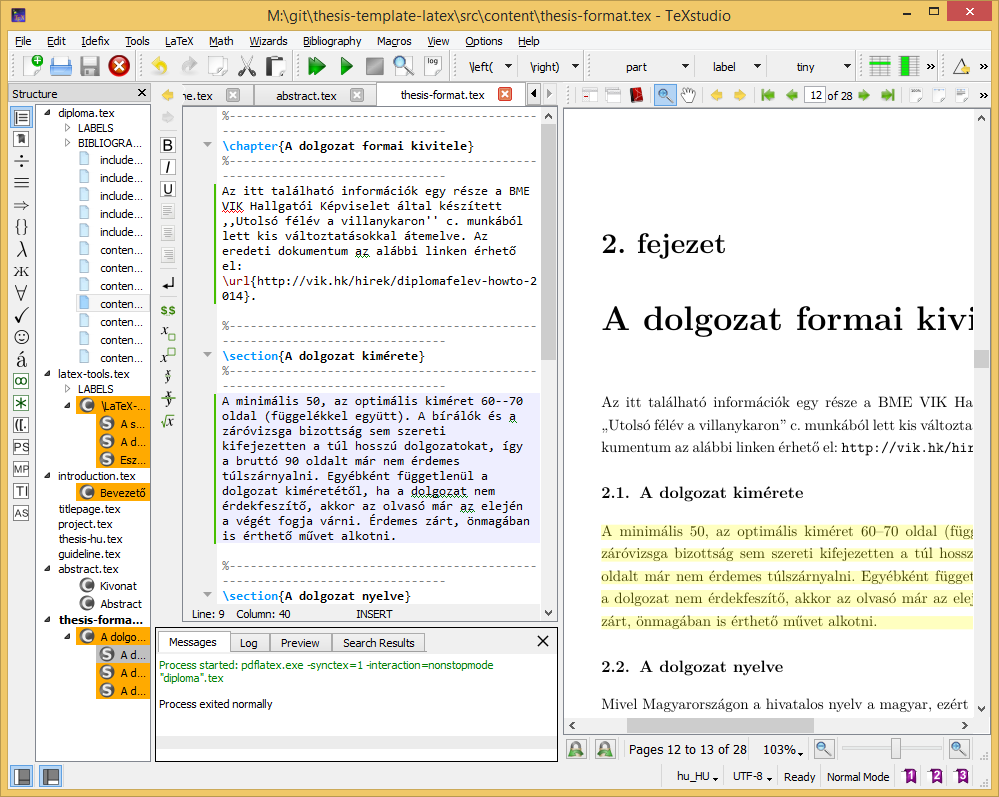
\includegraphics[width=67mm, keepaspectratio]{figures/TeXstudio.png}\hspace{1cm}
	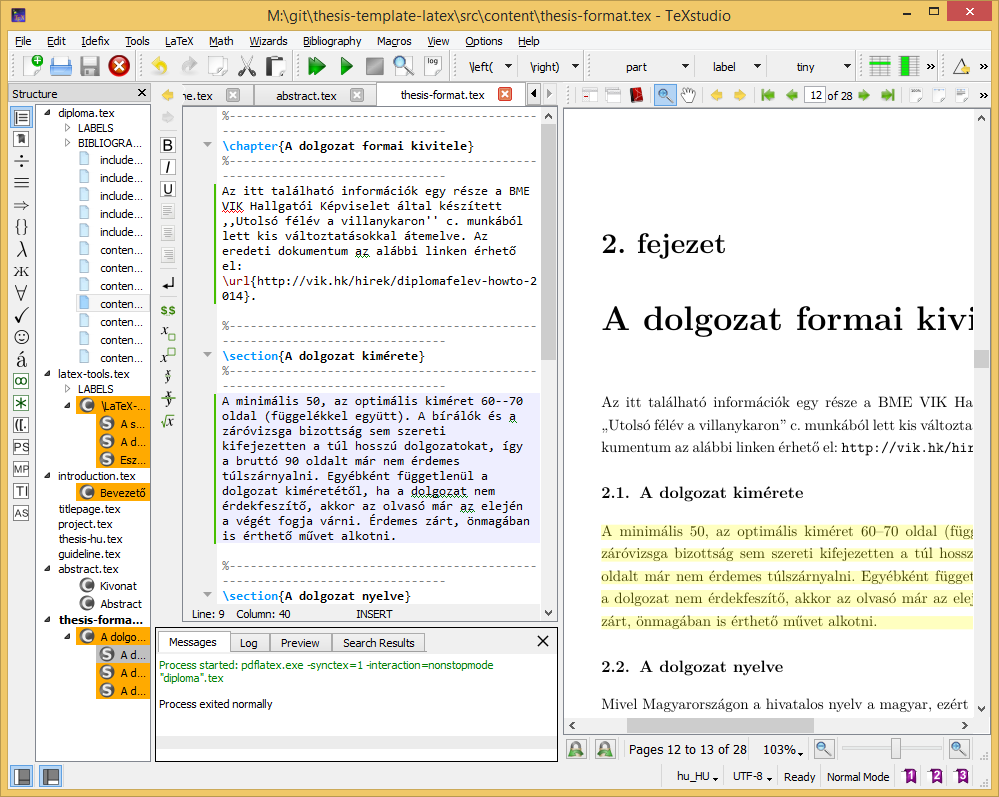
\includegraphics[width=67mm, keepaspectratio]{figures/TeXstudio.png}\\\vspace{5mm}
	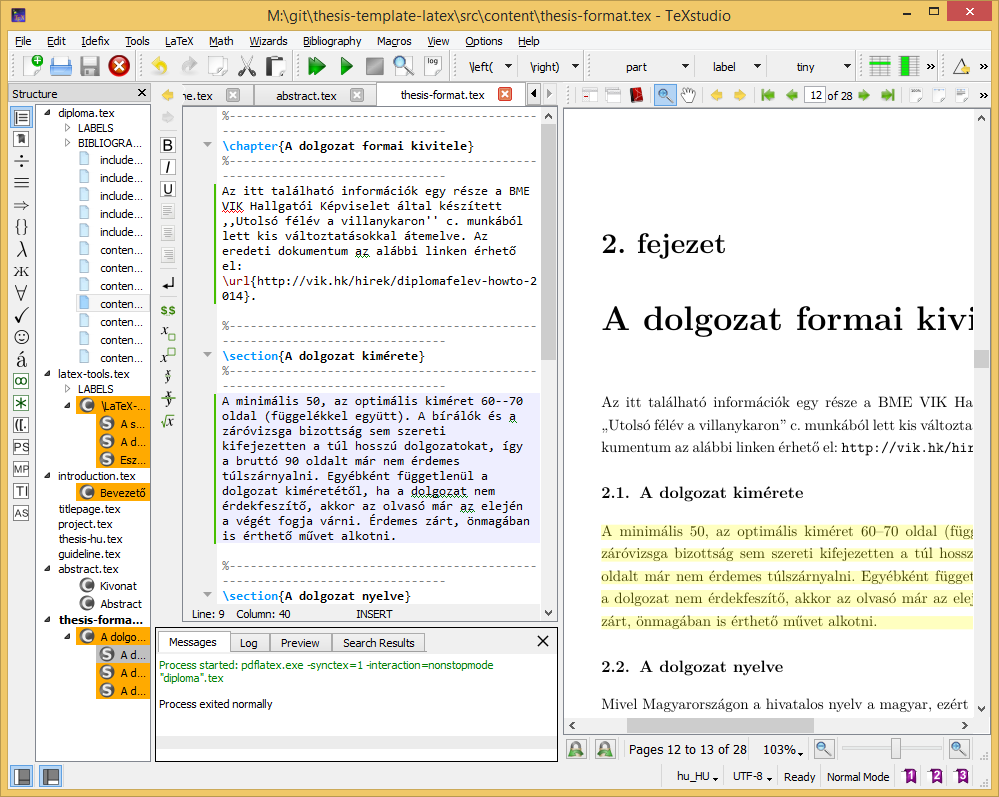
\includegraphics[width=67mm, keepaspectratio]{figures/TeXstudio.png}\hspace{1cm}
	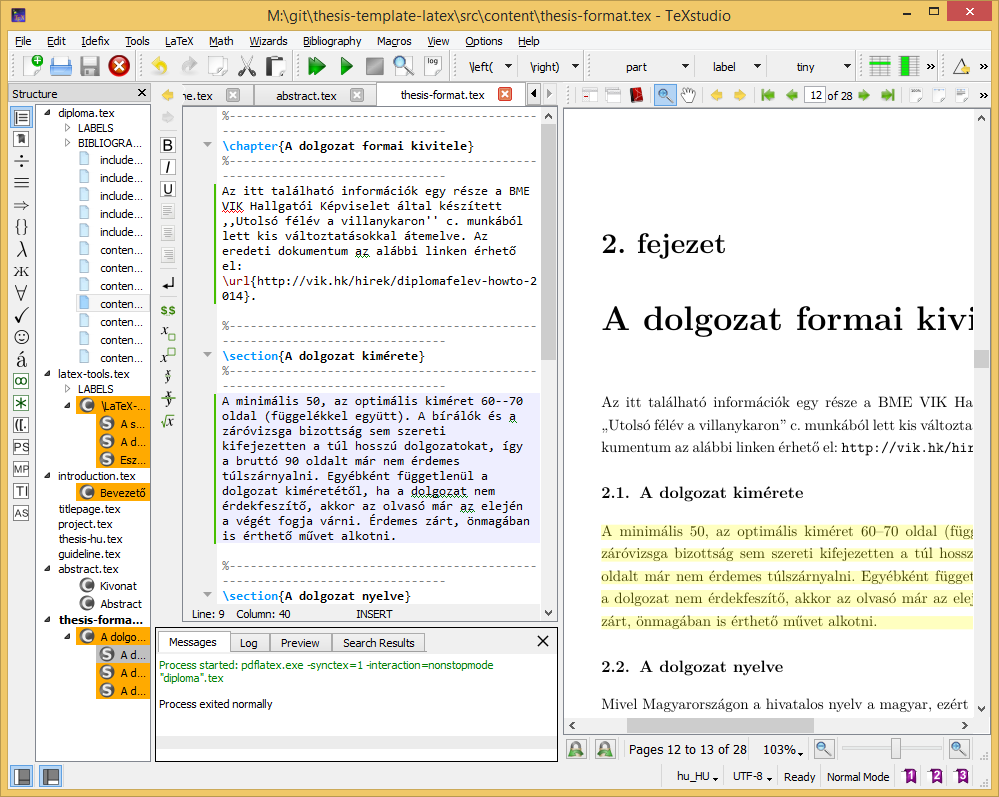
\includegraphics[width=67mm, keepaspectratio]{figures/TeXstudio.png}
	\caption{Több képfájl beillesztése esetén térközöket is érdemes használni.}
	\label{fig:HVSpaces}
\end{figure}

A táblázatok használatára \aref{tab:TabularExample}~táblázat mutat példát. A táblázatok formázásához hasznos tanácsokat találunk a \verb+booktabs+ csomag dokumentációjában.

\begin{table}[ht]
	\footnotesize
	\centering
	\begin{tabular}{ l c c }
		\toprule
		Órajel & Frekvencia & Cél pin \\
		\midrule
		CLKA & 100 MHz & FPGA CLK0\\
		CLKB & 48 MHz  & FPGA CLK1\\
		CLKC & 20 MHz  & Processzor\\
		CLKD & 25 MHz  & Ethernet chip \\
		CLKE & 72 MHz  & FPGA CLK2\\
		XBUF & 20 MHz  & FPGA CLK3\\
		\bottomrule
	\end{tabular}
	\caption{Az órajel-generátor chip órajel-kimenetei.}
	\label{tab:TabularExample}
\end{table}


%----------------------------------------------------------------------------
\section{Felsorolások és listák}
%----------------------------------------------------------------------------
Számozatlan felsorolásra mutat példát a jelenlegi bekezdés:
\begin{itemize}
	\item \emph{első bajusz:} ide lehetne írni az első elem kifejését,
	\item \emph{második bajusz:} ide lehetne írni a második elem kifejését,
	\item \emph{ez meg egy szakáll:} ide lehetne írni a harmadik elem kifejését.
\end{itemize}

Számozott felsorolást is készíthetünk az alábbi módon:
\begin{enumerate}
	\item \emph{első bajusz:} ide lehetne írni az első elem kifejését, és ez a kifejtés így néz ki, ha több sorosra sikeredik,
	\item \emph{második bajusz:} ide lehetne írni a második elem kifejését,
	\item \emph{ez meg egy szakáll:} ide lehetne írni a harmadik elem kifejését.
\end{enumerate}
A felsorolásokban sorok végén vessző, az utolsó sor végén pedig pont a szokásos írásjel. Ez alól kivételt képezhet, ha az egyes elemek több teljes mondatot tartalmaznak.

Listákban a dolgozat szövegétől elkülönítendő kódrészleteket, programsorokat, pszeudo-kódokat jeleníthetünk meg (\ref{lst:Example}.~kódrészlet).
\begin{lstlisting}[language=tex,caption=A fenti számozott felsorolás \LaTeX-forráskódja,label=lst:Example]
\begin{enumerate}
	\item \emph{els(*@ő@*) bajusz:} ide lehetne írni az els(*@ő@*) elem kifejését,
	és ez a kifejtés így néz ki, ha több sorosra sikeredik,
	\item \emph{második bajusz:} ide lehetne írni a második elem kifejését,
	\item \emph{ez meg egy szakáll:} ide lehetne írni a harmadik elem kifejését.
\end{enumerate}
\end{lstlisting}
A lista keretét, háttérszínét, egész stílusát megválaszthatjuk. Ráadásul különféle programnyelveket és a nyelveken belül kulcsszavakat is definiálhatunk, ha szükséges. Erről bővebbet a \verb+listings+ csomag hivatalos leírásában találhatunk.

%----------------------------------------------------------------------------
\section{Képletek}
%----------------------------------------------------------------------------
Ha egy formula nem túlságosan hosszú, és nem akarjuk hivatkozni a szövegből, mint például a $e^{i\pi}+1=0$ képlet, \emph{szövegközi képletként} szokás leírni. Csak, hogy másik példát is lássunk, az $U_i=-d\Phi/dt$ Faraday-törvény a $\rot E=-\frac{dB}{dt}$ differenciális alakban adott Maxwell-egyenlet felületre vett integráljából vezethető le. Látható, hogy a \LaTeX-fordító a sorközöket betartja, így a szöveg szedése esztétikus marad szövegközi képletek használata esetén is.

Képletek esetén az általános konvenció, hogy a kisbetűk skalárt, a kis félkövér betűk ($\mathbf{v}$) oszlopvektort -- és ennek megfelelően $\mathbf{v}^T$ sorvektort -- a kapitális félkövér betűk ($\mathbf{V}$) mátrixot jelölnek. Ha ettől el szeretnénk térni, akkor az alkalmazni kívánt jelölésmódot célszerű külön alfejezetben definiálni. Ennek megfelelően, amennyiben $\mathbf{y}$ jelöli a mérések vektorát, $\mathbf{\vartheta}$ a paraméterek vektorát és $\hat{\mathbf{y}}=\mathbf{X}\vartheta$ a paraméterekben lineáris modellt, akkor a \emph{Least-Squares} értelemben optimális paraméterbecslő $\hat{\mathbf{\vartheta}}_{LS}=(\mathbf{X}^T\mathbf{X})^{-1}\mathbf{X}^T\mathbf{y}$ lesz.

Emellett kiemelt, sorszámozott képleteket is megadhatunk, ennél az \verb+equation+ és a \verb+eqnarray+ környezetek helyett a korszerűbb \verb+align+ környezet alkalmazását javasoljuk (több okból, különféle problémák elkerülése végett, amelyekre most nem térünk ki). Tehát
\begin{align}
\dot{\mathbf{x}}&=\mathbf{A}\mathbf{x}+\mathbf{B}\mathbf{u},\\
\mathbf{y}&=\mathbf{C}\mathbf{x},
\end{align}
ahol $\mathbf{x}$ az állapotvektor, $\mathbf{y}$ a mérések vektora és $\mathbf{A}$, $\mathbf{B}$ és $\mathbf{C}$ a rendszert leíró paramétermátrixok. Figyeljük meg, hogy a két egyenletben az egyenlőségjelek egymáshoz igazítva jelennek meg, mivel a mindkettőt az \& karakter előzi meg a kódban. Lehetőség van számozatlan kiemelt képlet használatára is, például
\begin{align}
\dot{\mathbf{x}}&=\mathbf{A}\mathbf{x}+\mathbf{B}\mathbf{u},\nonumber\\
\mathbf{y}&=\mathbf{C}\mathbf{x}\nonumber.
\end{align}
Mátrixok felírására az $\mathbf{A}\mathbf{x}=\mathbf{b}$ inhomogén lineáris egyenlet részletes kifejtésével mutatunk példát:
\begin{align}
\begin{bmatrix}
a_{11} & a_{12} & \dots & a_{1n}\\
a_{21} & a_{22} & \dots & a_{2n}\\
\vdots & \vdots & \ddots & \vdots\\
a_{m1} & a_{m2} & \dots & a_{mn}
\end{bmatrix}
\begin{pmatrix}x_1\\x_2\\\vdots\\x_n\end{pmatrix}=
\begin{pmatrix}b_1\\b_2\\\vdots\\b_m\end{pmatrix}.
\end{align}
A \verb+\frac+ utasítás hatékonyságát egy általános másodfokú tag átviteli függvényén keresztül mutatjuk be, azaz
\begin{align}
W(s)=\frac{A}{1+2T\xi s+s^2T^2}.
\end{align}
A matematikai mód minden szimbólumának és képességének a bemutatására természetesen itt nincs lehetőség, de gyors referenciaként hatékonyan használhatók a következő linkek:\\
\indent\url{http://www.artofproblemsolving.com/LaTeX/AoPS_L_GuideSym.php},\\
\indent\url{http://www.ctan.org/tex-archive/info/symbols/comprehensive/symbols-a4.pdf},\\
\indent\url{ftp://ftp.ams.org/pub/tex/doc/amsmath/short-math-guide.pdf}.\\
Ez pedig itt egy magyarázat, hogy miért érdemes \verb+align+ környezetet használni:\\
\indent\url{http://texblog.net/latex-archive/maths/eqnarray-align-environment/}.

%----------------------------------------------------------------------------
\section{Irodalmi hivatkozások}
\label{sec:HowtoReference}
%----------------------------------------------------------------------------
Egy \LaTeX~dokumentumban az irodalmi hivatkozások definíciójának két módja van. Az egyik a \verb+\thebibliograhy+ környezet használata a dokumentum végén, az \verb+\end{document}+ lezárás előtt.
\begin{lstlisting}[language=tex]
\begin{thebibliography}{9}

\bibitem{Lamport94} Leslie Lamport, \emph{\LaTeX: A Document Preparation System}.
Addison Wesley, Massachusetts, 2nd Edition, 1994.

\end{thebibliography}
\end{lstlisting}

Ezek után a dokumentumban a \verb+\cite{Lamport94}+ utasítással hivatkozhatunk a forrásra. A fenti megadás viszonylag kötetlen, a szerző maga formázza az irodalomjegyzéket (ami gyakran inkonzisztens eredményhez vezet).

Egy sokkal professzionálisabb módszer a BiB\TeX{} használata, ezért ez a sablon is ezt támogatja. Ebben az esetben egy külön szöveges adatbázisban definiáljuk a forrásmunkákat, és egy külön stílusfájl határozza meg az irodalomjegyzék kinézetét. Ez, összhangban azzal, hogy külön formátumkonvenció határozza meg a folyóirat-, a könyv-, a konferenciacikk- stb. hivatkozások kinézetét az irodalomjegyzékben (a sablon használata esetén ezzel nem is kell foglalkoznia a hallgatónak, de az eredményt célszerű ellenőrizni). felhasznált hivatkozások adatbázisa egy \verb+.bib+ kiterjesztésű szöveges fájl, amelynek szerkezetét a \Aref{lst:Bibtex} kódrészlet demonstrálja. A forrásmunkák bevitelekor a sor végi vesszők külön figyelmet igényelnek, mert hiányuk a BiB\TeX-fordító hibaüzenetét eredményezi. A forrásmunkákat típus szerinti kulcsszó vezeti be (\verb+@book+ könyv, \verb+@inproceedings+ konferenciakiadványban megjelent cikk, \verb+@article+ folyóiratban megjelent cikk, \verb+@techreport+ valamelyik egyetem gondozásában megjelent műszaki tanulmány, \verb+@manual+ műszaki dokumentáció esetén stb.). Nemcsak a megjelenés stílusa, de a kötelezően megadandó mezők is típusról-típusra változnak. Egy jól használható referencia a \url{http://en.wikipedia.org/wiki/BibTeX} oldalon található.

\begin{lstlisting}[caption=Példa szöveges irodalomjegyzék-adatbázisra Bib\TeX{} használata esetén.,label=lst:Bibtex]
@book{Wettl04,
  author    = {Ferenc Wettl and Gyula Mayer and Péter Szabó},
  publisher = {Panem Könyvkiadó},
  title     = {\LaTeX~kézikönyv},
  year      = {2004},
}

@article{Candy86,
  author       = {James C. Candy},
  journaltitle = {{IEEE} Trans.\ on Communications},
  month        = {01},
  note         = {\doi{10.1109/TCOM.1986.1096432}},
  number       = {1},
  pages        = {72--76},
  title        = {Decimation for Sigma Delta Modulation},
  volume       = {34},
  year         = {1986},
}

@inproceedings{Lee87,
  author    = {Wai L. Lee and Charles G. Sodini},
  booktitle = {Proc.\ of the IEEE International Symposium on Circuits and Systems},
  location  = {Philadelphia, PA, USA},
  month     = {05~4--7},
  pages     = {459--462},
  title     = {A Topology for Higher Order Interpolative Coders},
  vol       = {2},
  year      = {1987},
}

@thesis{KissPhD,
  author      = {Peter Kiss},
  institution = {Technical University of Timi\c{s}oara, Romania},
  month       = {04},
  title       = {Adaptive Digital Compensation of Analog Circuit Imperfections for Cascaded Delta-Sigma Analog-to-Digital Converters},
  type        = {phdthesis},
  year        = {2000},
}

@manual{Schreier00,
  author       = {Richard Schreier},
  month        = {01},
  note         = {\url{http://www.mathworks.com/matlabcentral/fileexchange/}},
  organization = {Oregon State University},
  title        = {The Delta-Sigma Toolbox v5.2},
  year         = {2000},
}

@misc{DipPortal,
  author       = {{Budapesti Műszaki és Gazdaságtudományi Egyetem Villamosmérnöki és Informatikai Kar}},
  howpublished = {\url{http://diplomaterv.vik.bme.hu/}},
  title        = {Diplomaterv portál (2011. február 26.)},
}

@incollection{Mkrtychev:1997,
  author    = {Mkrtychev, Alexey},
  booktitle = {Logical Foundations of Computer Science},
  doi       = {10.1007/3-540-63045-7_27},
  editor    = {Adian, Sergei and Nerode, Anil},
  isbn      = {978-3-540-63045-6},
  pages     = {266-275},
  publisher = {Springer Berlin Heidelberg},
  series    = {Lecture Notes in Computer Science},
  title     = {Models for the logic of proofs},
  url       = {http://dx.doi.org/10.1007/3-540-63045-7_27},
  volume    = {1234},
  year      = {1997},
}
\end{lstlisting}

A stílusfájl egy \verb+.sty+ kiterjesztésű fájl, de ezzel lényegében nem kell foglalkozni, mert vannak beépített stílusok, amelyek jól használhatók. Ez a sablon a BiB\TeX-et használja, a hozzá tartozó adatbázisfájl a \verb+mybib.bib+ fájl. Megfigyelhető, hogy az irodalomjegyzéket a dokumentum végére (a \verb+\end{document}+ utasítás elé) beillesztett \verb+\bibliography{mybib}+ utasítással hozhatjuk létre, a stílusát pedig ugyanitt a  \verb+\bibliographystyle{plain}+ utasítással adhatjuk meg. Ebben az esetben a \verb+plain+ előre definiált stílust használjuk (a sablonban is ezt állítottuk be). A \verb+plain+ stíluson kívül természetesen számtalan más előre definiált stílus is létezik. Mivel a \verb+.bib+ adatbázisban ezeket megadtuk, a BiB\TeX-fordító is meg tudja különböztetni a szerzőt a címtől és a kiadótól, és ez alapján automatikusan generálódik az irodalomjegyzék a stílusfájl által meghatározott stílusban.

Az egyes forrásmunkákra a szövegből továbbra is a \verb+\cite+ paranccsal tudunk hivatkozni, így \aref{lst:Bibtex}.~kódrészlet esetén a hivatkozások rendre \verb+\cite{Wettl04}+, \verb+\cite{Candy86}+, \verb+\cite{Lee87}+, \verb+\cite{KissPhD}+, \verb+\cite{Schreirer00}+,
\verb+\cite{Mkrtychev:1997}+ és \verb+\cite{DipPortal}+. Az egyes forrásmunkák sorszáma az irodalomjegyzék bővítésekor változhat. Amennyiben az aktuális számhoz illeszkedő névelőt szeretnénk használni, használjuk az \verb+\acite{}+ parancsot.

Az irodalomjegyzékben alapértelmezésben csak azok a forrásmunkák jelennek meg, amelyekre található hivatkozás a szövegben, és ez így alapvetően helyes is, hiszen olyan forrásmunkákat nem illik az irodalomjegyzékbe írni, amelyekre nincs hivatkozás.

Mivel a fordítási folyamat során több lépésben oldódnak fel a szimbólumok, ezért gyakran többször is le kell fordítani a dokumentumot. Ilyenkor ez első 1-2 fordítás esetleg szimbólum-feloldásra vonatkozó figyelmeztető üzenettel zárul. Ha hibaüzenettel zárul bármelyik fordítás, akkor nincs értelme megismételni, hanem a hibát kell megkeresni. A \verb+.bib+ fájl megváltoztatáskor sokszor nincs hatása a változtatásnak azonnal, mivel nem mindig fut újra a BibTeX fordító. Ezért célszerű a változtatás után azt manuálisan is lefuttatni (TeXstudio esetén \verb+Tools/Bibliography+).

Hogy a szövegbe ágyazott hivatkozások kinézetét demonstráljuk, itt most sorban meghivatkozzuk a \cite{Wettl04}, \cite{Candy86}, \cite{Lee87}, \cite{KissPhD}, \cite{Schreier00} és \acite{Mkrtychev:1997}\footnote{Informatikai témában gyakran hivatkozunk cikkeket a Springer LNCS valamely kötetéből, ez a hivatkozás erre mutat egy helyes példát.} forrásmunkát, valamint \acite{DipPortal} weboldalt.

Megjegyzendő, hogy az ékezetes magyar betűket is tartalmazó \verb+.bib+ fájl az \verb+inputenc+ csomaggal betöltött \verb+latin2+ betűkészlet miatt fordítható. Ugyanez a \verb+.bib+ fájl hibaüzenettel fordul egy olyan dokumentumban, ami nem tartalmazza a \verb+\usepackage[latin2]{inputenc}+ sort. Speciális igény esetén az irodalmi adatbázis általánosabb érvényűvé tehető, ha az ékezetes betűket speciális latex karakterekkel helyettesítjük a \verb+.bib+ fájlban, pl. á helyett \verb+\'{a}+-t vagy ő helyett \verb+\H{o}+-t írunk.

Irodalomhivatkozásokat célszerű először olyan szolgáltatásokban keresni, ahol jó minőségű bejegyzések találhatók (pl. ACM Digital Library,\footnote{\url{https://dl.acm.org/}} DBLP,\footnote{\url{http://dblp.uni-trier.de/}} IEEE Xplore,\footnote{\url{http://ieeexplore.ieee.org/}} SpringerLink\footnote{\url{https://link.springer.com/}}) és csak ezek után használni kevésbé válogatott forrásokat (pl. Google Scholar\footnote{\url{http://scholar.google.com/}}). A jó minőségű bejegyzéseket is érdemes megfelelően tisztítani.\footnote{\url{https://github.com/FTSRG/cheat-sheets/wiki/BibTeX-Fixing-entries-from-common-sources}} A sablon angol nyelvű változatában használt \texttt{plainnat} beállítás egyik sajátossága, hogy a cikkhez generált hivatkozás a cikk DOI-ját és URL-jét is tartalmazza, ami gyakran duplikátumhoz vezet -- érdemes tehát a DOI-kat tartalmazó URL mezőket törölni. 

%----------------------------------------------------------------------------
\section{A dolgozat szerkezete és a forrásfájlok}
%----------------------------------------------------------------------------
A diplomatervsablonban a TeX fájlok két alkönyvtárban helyezkednek el. Az \verb+include+ könyvtárban azok szerepelnek, amiket tipikusan nem kell szerkesztenünk, ezek a sablon részei (pl. címoldal). A \verb+content+ alkönyvtárban pedig a saját munkánkat helyezhetjük el. Itt érdemes az egyes fejezeteket külön \TeX{} állományokba rakni.

A diplomatervsablon (a kari irányelvek szerint) az alábbi fő fejezetekből áll:
\begin{enumerate}
	\item 1 oldalas \emph{tájékoztató} a szakdolgozat/diplomaterv szerkezetéről (\verb+include/guideline.tex+), ami a végső dolgozatból törlendő,
	\item \emph{feladatkiírás} (\verb+include/project.tex+), a dolgozat nyomtatott verzójában ennek a helyére kerül a tanszék által kiadott, a tanszékvezető által aláírt feladatkiírás, a dolgozat elektronikus verziójába pedig a feladatkiírás egyáltalán ne kerüljön bele, azt külön tölti fel a tanszék a diplomaterv-honlapra,
	\item \emph{címoldal} (\verb+include/titlepage.tex+),
	\item \emph{tartalomjegyzék} (\verb+thesis.tex+),
	\item a diplomatervező \emph{nyilatkozat}a az önálló munkáról (\verb+include/declaration.tex+),
	\item 1-2 oldalas tartalmi \emph{összefoglaló} magyarul és angolul, illetve elkészíthető még további nyelveken is (\verb+content/abstract.tex+),
	\item \emph{bevezetés}: a feladat értelmezése, a tervezés célja, a feladat indokoltsága, a diplomaterv felépítésének rövid összefoglalása (\verb+content/introduction.tex+),
	\item sorszámmal ellátott \emph{fejezetek}: a feladatkiírás pontosítása és részletes elemzése, előzmények (irodalomkutatás, hasonló alkotások), az ezekből levonható következtetések, a tervezés részletes leírása, a döntési lehetőségek értékelése és a választott megoldások indoklása, a megtervezett műszaki alkotás értékelése, kritikai elemzése, továbbfejlesztési lehetőségek,
	\item esetleges \emph{köszönetnyilvánítás}ok (\verb+content/acknowledgement.tex+),
	\item részletes és pontos \emph{irodalomjegyzék} (ez a sablon esetében automatikusan generálódik a \verb+thesis.tex+ fájlban elhelyezett \verb+\bibliography+ utasítás hatására, \az+\refstruc{sec:HowtoReference}ban leírtak szerint),
	\item \emph{függelékek} (\verb+content/appendices.tex+).
\end{enumerate}

A sablonban a fejezetek a \verb+thesis.tex+ fájlba vannak beillesztve \verb+\include+ utasítások segítségével. Lehetőség van arra, hogy csak az éppen szerkesztés alatt álló \verb+.tex+ fájlt fordítsuk le, ezzel lerövidítve a fordítási folyamatot. Ezt a lehetőséget az alábbi kódrészlet biztosítja a \verb+thesis.tex+ fájlban.
\begin{lstlisting}
\includeonly{
	guideline,%
	project,%
	titlepage,%
	declaration,%
	abstract,%
	introduction,%
	chapter1,%
	chapter2,%
	chapter3,%
	acknowledgement,%
	appendices,%
}
\end{lstlisting}

Ha az alábbi kódrészletben az egyes sorokat a \verb+%+ szimbólummal kikommentezzük, akkor a megfelelő \verb+.tex+ fájl nem fordul le. Az oldalszámok és a tartalomjegyék természetesen csak akkor billennek helyre, ha a teljes dokumentumot lefordítjuk.

%----------------------------------------------------------------------------
\newpage
\section{Alapadatok megadása}
%----------------------------------------------------------------------------
A diplomaterv alapadatait (cím, szerző, konzulens, konzulens titulusa) a \verb+thesis.tex+ fájlban lehet megadni.

%----------------------------------------------------------------------------
\section{Új fejezet írása}
%----------------------------------------------------------------------------
A főfejezetek külön \verb+content+ könyvtárban foglalnak helyet. A sablonhoz 3 fejezet készült. További főfejezeteket úgy hozhatunk létre, ha új \TeX~fájlt készítünk a fejezet számára, és a \verb+thesis.tex+ fájlban, a \verb+\include+ és \verb+\includeonly+ utasítások argumentumába felvesszük az új \verb+.tex+ fájl nevét.


%----------------------------------------------------------------------------
\section{Definíciók, tételek, példák}
%----------------------------------------------------------------------------

\begin{definition}[Fluxuskondenzátor térerőssége]
Lorem ipsum dolor sit amet, consectetur adipiscing elit, sed do eiusmod tempor incididunt ut labore et dolore magna aliqua. Ut enim ad minim veniam, quis nostrud exercitation ullamco laboris nisi ut aliquip ex ea commodo consequat.
\end{definition}

\begin{example}
Példa egy példára. Duis aute irure dolor in reprehenderit in voluptate velit esse cillum dolore eu fugiat nulla pariatur. Excepteur sint occaecat cupidatat non proident, sunt in culpa qui officia deserunt mollit anim id est laborum.
\end{example}

\begin{theorem}[Kovács tétele]
Duis aute irure dolor in reprehenderit in voluptate velit esse cillum dolore eu fugiat nulla pariatur. Excepteur sint occaecat cupidatat non proident, sunt in culpa qui officia deserunt mollit anim id est laborum.
\end{theorem}



% Acknowledgements
%~~~~~~~~~~~~~~~~~~~~~~~~~~~~~~~~~~~~~~~~~~~~~~~~~~~~~~~~~~~~~~~~~~~~~~~~~~~~~~~~~~~~~~
%%----------------------------------------------------------------------------
\chapter*{\koszonetnyilvanitas}\addcontentsline{toc}{chapter}{\koszonetnyilvanitas}
%----------------------------------------------------------------------------

Ez nem kötelező, akár törölhető is. Ha a szerző szükségét érzi, itt lehet köszönetet nyilvánítani azoknak, akik hozzájárultak munkájukkal ahhoz, hogy a hallgató a szakdolgozatban vagy diplomamunkában leírt feladatokat sikeresen elvégezze. A konzulensnek való köszönetnyilvánítás sem kötelező, a konzulensnek hivatalosan is dolga, hogy a hallgatót konzultálja.


% List of Figures, Tables
%~~~~~~~~~~~~~~~~~~~~~~~~~~~~~~~~~~~~~~~~~~~~~~~~~~~~~~~~~~~~~~~~~~~~~~~~~~~~~~~~~~~~~~
%\listoffigures\addcontentsline{toc}{chapter}{\listfigurename}
%\listoftables\addcontentsline{toc}{chapter}{\listtablename}


% Bibliography
%~~~~~~~~~~~~~~~~~~~~~~~~~~~~~~~~~~~~~~~~~~~~~~~~~~~~~~~~~~~~~~~~~~~~~~~~~~~~~~~~~~~~~~
\addcontentsline{toc}{chapter}{\bibname}
\bibliography{bib/mybib}


% Appendix
%~~~~~~~~~~~~~~~~~~~~~~~~~~~~~~~~~~~~~~~~~~~~~~~~~~~~~~~~~~~~~~~~~~~~~~~~~~~~~~~~~~~~~~
%%----------------------------------------------------------------------------
\appendix
%----------------------------------------------------------------------------
\chapter*{\fuggelek}\addcontentsline{toc}{chapter}{\fuggelek}
\setcounter{chapter}{\appendixnumber}
%\setcounter{equation}{0} % a fofejezet-szamlalo az angol ABC 6. betuje (F) lesz
\numberwithin{equation}{section}
\numberwithin{figure}{section}
\numberwithin{lstlisting}{section}
%\numberwithin{tabular}{section}

%----------------------------------------------------------------------------
\section{A TeXstudio felülete}
%----------------------------------------------------------------------------
\begin{figure}[!ht]
\centering
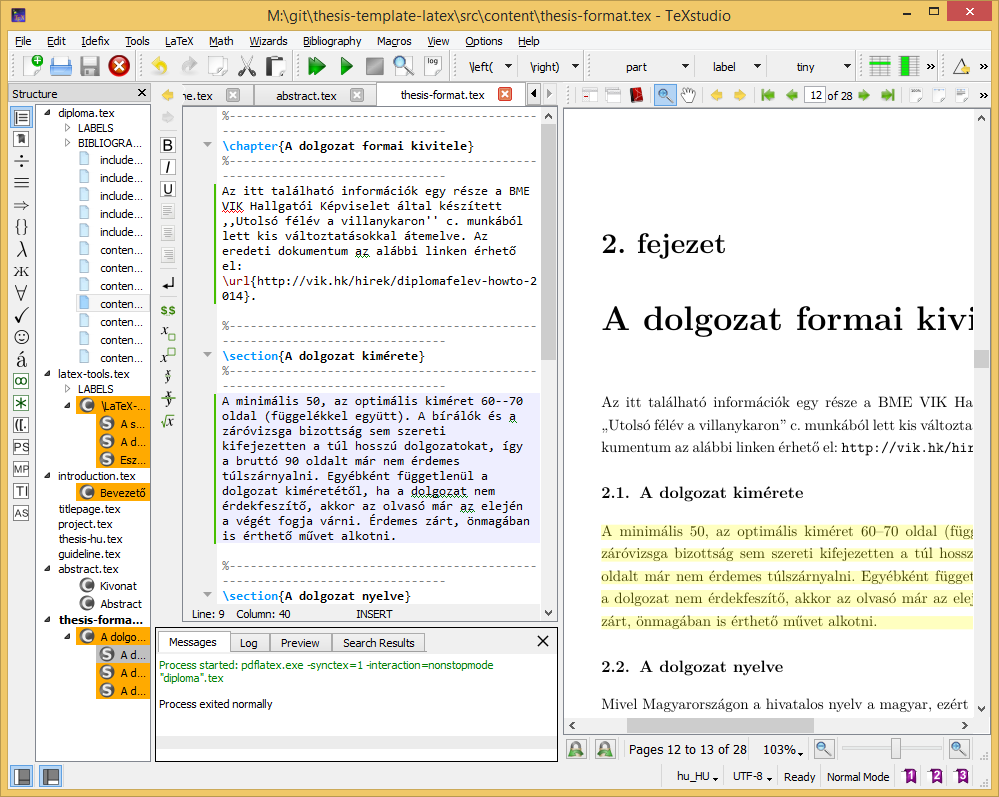
\includegraphics[width=150mm, keepaspectratio]{figures/TeXstudio.png}
\caption{A TeXstudio \LaTeX-szerkesztő.} 
\end{figure}

%----------------------------------------------------------------------------
\clearpage\section{Válasz az ,,Élet, a világmindenség, meg minden'' kérdésére}
%----------------------------------------------------------------------------
A Pitagorasz-tételből levezetve
\begin{align}
c^2=a^2+b^2=42.
\end{align}
A Faraday-indukciós törvényből levezetve
\begin{align}
\rot E=-\frac{dB}{dt}\hspace{1cm}\longrightarrow \hspace{1cm}
U_i=\oint\limits_\mathbf{L}{\mathbf{E}\mathbf{dl}}=-\frac{d}{dt}\int\limits_A{\mathbf{B}\mathbf{da}}=42.
\end{align}


%\label{page:last}
\end{document}
